\documentclass[DIV15,BCOR12mm]{scrbook}
\newif\ifAFive\AFivetrue
\ifAFive
  \KOMAoptions{paper=a5,twoside=true}
\else
  \KOMAoptions{paper=a4,twoside=false}
\fi
\usepackage{etoolbox}
\usepackage{amsmath,amssymb}% math symbols / fonts
\usepackage{mathtools}      % \xRightarrow
\usepackage{nicefrac}       % \nicefrac
\usepackage[utf8]{inputenc} % this is needed for umlauts
\usepackage[ngerman]{babel} % this is needed for umlauts
\usepackage[T1]{fontenc}    % this is needed for correct output of umlauts in pdf
\usepackage[framed,amsmath,thmmarks,hyperref]{ntheorem}
\usepackage{framed}
\usepackage{marvosym}
\usepackage{makeidx}        % for automatically generation of an index
\usepackage{xcolor}
\usepackage[bookmarks,bookmarksnumbered,hypertexnames=false,pdfpagelayout=OneColumn,colorlinks,hyperindex=false]{hyperref} % has to be after makeidx
\usepackage{breakurl} % allow line breaks in \href{ ... }
\ifAFive
  \hypersetup{hidelinks=true}
% no \else branch needed in this case
\fi
\usepackage{enumitem}       % Better than \usepackage{enumerate}, because it allows to set references
\usepackage{tabto}
\usepackage{braket}         % needed for \Set
\usepackage{csquotes}       % \enquote{}
\usepackage{subfig}         % multiple figures in one
\usepackage{parskip}        % nicer paragraphs
\usepackage{xifthen}        % \isempty
\usepackage{changepage}     % for the adjustwidth environment
\usepackage{pst-solides3d}
\usepackage[colorinlistoftodos]{todonotes}
\usepackage{pgfplots}
\pgfplotsset{compat=1.7}
\usepackage[arrow, matrix, curve]{xy}
\usepackage{caption}        % get newlines within captions
\usepackage{tikz}           % draw
\usepackage{tikz-3dplot}    % draw
\usepackage{tkz-fct}        % draw
\usepackage{tkz-euclide}    % draw
\usetkzobj{all}             % tkz-euclide
\usetikzlibrary{3d,calc,intersections,er,arrows,positioning,shapes.misc,patterns,fadings,decorations.pathreplacing}
\usepackage{tqft}
\usepackage{xspace}   % for new commands; decides weather I want to insert a space after the command
\usepackage[german,nameinlink]{cleveref} % has to be after hyperref, ntheorem, amsthm
%%%%%%%%%%%%%%%%%%%%%%%%%%%%%%%%%%%%%%%%%%%%%%%%%%%%%%%%%%%%%%%%%%%%%%%%%%%%%%%%
\usepackage{array,xtab,ragged2e} % for symbol table
\newlength\mylengtha
\newlength\mylengthb
\newcolumntype{P}[1]{>{\RaggedRight}p{#1}}
\tabcolsep=3pt % default: 6pt
%%%%%%%%%%%%%%%%%%%%%%%%%%%%%%%%%%%%%%%%%%%%%%%%%%%%%%%%%%%%%%%%%%%%%%%%%%%%%%%%
\usepackage{acronym}
\usepackage{minted} % needed for the inclusion of source code
\usemintedstyle{bw}
\usepackage{courier}
\usepackage{wasysym}
\usepackage[binary-units = true]{siunitx} % this package is for units!
\sisetup{locale=DE}

%%% Pseudocode settings
\usepackage{algorithm,algpseudocode}
\algtext*{EndIf}        % Remove "end if" text
\algtext*{EndWhile}     % Remove "end while" text
\algtext*{EndFunction}  % Remove "end while" text
\algnewcommand\Global{\textbf{global }}
\makeatletter
\addto\captionsngerman{\renewcommand{\ALG@name}{Algorithmus}}
\makeatother
%%% End of Pseudocode settings
\usepackage{shortcuts}

\usepackage{fancyhdr}
\pagestyle{fancy}
\renewcommand{\chaptermark}[1]%
{\markboth{\MakeUppercase{\thechapter.\ #1}}{}}
\renewcommand{\sectionmark}[1]%
{\markright{\MakeUppercase{\thesection.\ #1}}}
\renewcommand{\headrulewidth}{0.5pt}
\renewcommand{\footrulewidth}{0pt}
\newcommand{\helv}{%
\fontfamily{phv}\fontseries{b}\fontsize{9}{11}\selectfont}
\fancyhf{}
\fancyhead[LO,RE]{\helv \thepage}
\fancyhead[LE]{\helv \rightmark}
\fancyhead[RO]{\helv \leftmark}
\fancypagestyle{plain}{%
\fancyhead{}
\renewcommand{\headrulewidth}{0pt}
}

\hypersetup{ 
  pdfauthor   = {Martin Thoma}, 
  pdfkeywords = {Programmierparadigmen}, 
  pdftitle    = {Programmierparadigmen} 
}
%%%%%%%%%%%%%%%%%%%%%%%%%%%%%%%%%%%%%%%%%%%%%%%%%%%%%%%%%%%%%%%%%%%%%%%%%%%%%%%%
% The patch for minted: http://tex.stackexchange.com/a/168021/5645
\makeatletter
\def\FV@BeginListFrame@Lines{%
  \begingroup
  \lineskip\z@skip
  \FV@SingleFrameLine{\z@}%
  \kern-0.5\baselineskip\relax
  \baselineskip\z@skip
  \kern\FV@FrameSep\relax
  \penalty\@M% added line
\endgroup}
\makeatother
%%%%%%%%%%%%%%%%%%%%%%%%%%%%%%%%%%%%%%%%%%%%%%%%%%%%%%%%%%%%%%%%%%%%%%%%%%%%%%%%


\makeindex
\allowdisplaybreaks
\usepackage{microtype}

\begin{document}
%-------------------------------------------------------------
\newcolumntype{C}{>{\centering\arraybackslash}p{2cm}}
%-------------------------------------------------------------
\pagenumbering{roman}
\setcounter{page}{1}
\begin{titlepage}
\thispagestyle{empty}
\ifAFive
    \par\vspace{4cm}
\else
    \par\vspace{10cm}
\fi
\begin{center}
{\Large \textbf{Einführung in die}} \\[2ex]
{\Large \textbf{Geometrie und Topologie}}
\vfill

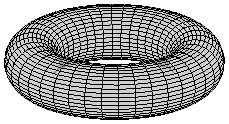
\includegraphics[width=0.9\linewidth]{figures/Torus.pdf}
\vfill
\hrulefill
\end{center}
\ \\[-5ex]
0. Auflage, \today \hfill Martin Thoma
\end{titlepage}

\chapter*{Vorwort}
Dieses Skript wird/wurde im Wintersemester 2013/2014 geschrieben.
Es beinhaltet Vorlesungsnotizen von Studenten zur Vorlesung von
Prof. Dr. Herrlich.

Es darf jeder gerne Verbesserungen einbringen!

Die Kurz-URL des Projekts lautet \href{http://tinyurl.com/GeoTopo}{tinyurl.com/GeoTopo}.

An dieser Stelle möchte ich noch Herrn Prof. Dr. Herrlich 
für einige Korrekturvorschläge und einen gut strukturierten 
Tafelanschrieb danken, der als Vorlage für dieses Skript diente.
Vielen Dank auch an Frau Lenz und Frau Randecker, die es mir erlaubt 
haben, ihre Übungsaufgaben und Lösungen zu benutzen.


\section*{Was ist Topologie?}

Die Kugeloberfläche $S^2$ lässt sich durch strecken, stauchen
und umformen zur Würfeloberfläche oder
der Oberfläche einer Pyramide verformen, aber nicht zum $\mdr^2$
oder zu einem Torus $T^2$. Für den $\mdr^2$ müsste man die Oberfläche
unendlich ausdehnen und für einen Torus müsste man ein Loch machen.

\begin{figure}[ht]
    \centering
    \subfloat[$S^2$]{
        % Source: http://tex.stackexchange.com/a/42865/5645
\begin{tikzpicture}
    \draw (-1,0) arc (180:360:1cm and 0.5cm);
    \draw[dashed] (-1,0) arc (180:0:1cm and 0.5cm);
    \draw (0,1) arc (90:270:0.5cm and 1cm);
    \draw[dashed] (0,1) arc (90:-90:0.5cm and 1cm);
    \draw (0,0) circle (1cm);
    \shade[ball color=blue!10!white,opacity=0.20] (0,0) circle (1cm);
\end{tikzpicture}

        \label{fig:s2}
    }%
    \subfloat[Würfel]{
        % Source: http://tex.stackexchange.com/a/12069/5645
\begin{tikzpicture}[scale=0.5]
   \clip (-3,-3) rectangle (3,3);
   \coordinate (tf) at (0,0);
   \coordinate (bf) at (0,-3);
   \coordinate (tr) at (15:2.5cm);
   \coordinate (tl) at (165:2.5cm);

   % You can change the perspective by playing with the 5, 5, 15:
   \coordinate (fr) at ($ (tf)!5!(tr) $);
   \coordinate (fl) at ($ (tf)!5!(tl) $);
   \coordinate (fb) at ($ (tf)!15!(bf) $);

   \path[name path=brpath] (bf) -- (fr);
   \path[name path=rbpath] (tr) -- (fb);
   \path[name path=blpath] (bf) -- (fl);
   \path[name path=lbpath] (tl) -- (fb);
   \path[name path=trpath] (tl) -- (fr);
   \path[name path=tlpath] (tr) -- (fl);

   \draw[name intersections={of=brpath and rbpath}] (intersection-1)coordinate (br){}; 
   \draw[name intersections={of=blpath and lbpath}] (intersection-1)coordinate (bl){}; 
   \draw[name intersections={of=trpath and tlpath}] (intersection-1)coordinate (tb){}; 

   \shade[right color=gray!10, left color=black!50, shading angle=105] (tf) -- (bf) -- (bl) -- (tl) -- cycle;
   \shade[left color=gray!10, right color=black!50, shading angle=75] (tf) -- (bf) -- (br) -- (tr) -- cycle;

   \begin{scope}
      \clip (tf) -- (tr) -- (tb) -- (tl) -- cycle;
      \shade[inner color = gray!5, outer color=black!50, shading=radial] (tf) ellipse (3cm and 1.5cm);
   \end{scope}

   \draw (tf) -- (bf);
   \draw (tf) -- (tr);
   \draw (tf) -- (tl);
   \draw (tr) -- (br);
   \draw (bf) -- (br);
   \draw (tl) -- (bl);
   \draw (bf) -- (bl);
   \draw (tb) -- (tr);
   \draw (tb) -- (tl);

   %set the sizes of the little cubes:
   \def\tone{.4}\def\ttwo{.75}\def\fone{.36}\def\ftwo{.70}
   \draw ($ (bf)!\tone!(br) $) -- ($ (tf)!\tone!(tr) $) -- ($ (tl)!\tone!(tb) $);
   \draw ($ (bf)!\ttwo!(br) $) -- ($ (tf)!\ttwo!(tr) $) -- ($ (tl)!\ttwo!(tb) $);
   \draw ($ (bf)!\tone!(bl) $) -- ($ (tf)!\tone!(tl) $) -- ($ (tr)!\tone!(tb) $);
   \draw ($ (bf)!\ttwo!(bl) $) -- ($ (tf)!\ttwo!(tl) $) -- ($ (tr)!\ttwo!(tb) $);
   \draw ($ (tl)!\fone!(bl) $) -- ($ (tf)!\fone!(bf) $) -- ($ (tr)!\fone!(br) $);
   \draw ($ (tl)!\ftwo!(bl) $) -- ($ (tf)!\ftwo!(bf) $) -- ($ (tr)!\ftwo!(br) $);
\end{tikzpicture}

        \label{fig:cube}
    }%
    \subfloat[Pyramide]{
        \begin{tikzpicture}[scale=.5, z={(.707,.3)}]
    \draw (2,3,2) -- (0,0,0) -- (4,0,0) -- (4,0,4) -- (2,3,2) 
      -- (4,0,0);
    \draw[color=gray, style=dashed] (2,3,2) -- (0,0,4) 
      -- (0,0,0);
    \draw[color=gray, style=dashed] (0,0,4) -- (4,0,4);
  \end{tikzpicture}

        \label{fig:pyramide}
    }

    \subfloat[$\mdr^2$]{
        \documentclass[varwidth=true, border=2pt]{standalone}
\usepackage{tikz}
\usepackage{tikz-3dplot}

\begin{document}
\tdplotsetmaincoords{110}{50}
\begin{tikzpicture}
		[tdplot_main_coords,
			cube/.style={very thick,black},
			grid/.style={very thin,gray},
			axis/.style={->,blue,thick}]

	%draw a grid in the x-y plane
	\foreach \x in {-0.5,0,...,2.5}
		\foreach \y in {-0.5,0,...,2.5}
		{
			\draw[grid] (\x,-0.5) -- (\x,2.5);
			\draw[grid] (-0.5,\y) -- (2.5,\y);
		}
			

	%draw the axes
	\draw[axis] (-1,0,0) -- (3,0,0) node[anchor=west]{$y$};
	\draw[axis] (0,-1,0) -- (0,3,0) node[anchor=west]{$x$};
	
\end{tikzpicture}
\end{document}

        \label{fig:plane-r2}
    }%
    \subfloat[$T^2$]{
        % Sketch output, version 0.3 (build 7d, Wed May 2 04:54:35 2012)
% Output language: PGF/TikZ,LaTeX
\begin{tikzpicture}[line join=round]
\filldraw[draw=black,fill=lightgray,fill opacity=0.75](-.048,.046)--(-.05,.045)--(.146,.042)--(.138,.044)--cycle;
\filldraw[draw=black,fill=lightgray,fill opacity=0.75](-.232,.038)--(-.246,.036)--(-.05,.045)--(-.048,.046)--cycle;
\filldraw[draw=black,fill=lightgray,fill opacity=0.75](.138,.044)--(.146,.042)--(.339,.028)--(.32,.031)--cycle;
\filldraw[draw=black,fill=lightgray,fill opacity=0.75](-.411,.02)--(-.435,.017)--(-.246,.036)--(-.232,.038)--cycle;
\filldraw[draw=black,fill=lightgray,fill opacity=0.75](.435,.951)--(.417,.954)--(.643,.923)--(.672,.919)--cycle;
\filldraw[draw=black,fill=lightgray,fill opacity=0.75](-.302,.964)--(-.288,.954)--(-.059,.964)--(-.062,.974)--cycle;
\filldraw[draw=black,fill=lightgray,fill opacity=0.75](-.062,.974)--(-.059,.964)--(.171,.961)--(.179,.971)--cycle;
\filldraw[draw=black,fill=lightgray,fill opacity=0.75](.179,.971)--(.171,.961)--(.397,.944)--(.417,.954)--cycle;
\filldraw[draw=black,fill=lightgray,fill opacity=0.75](-.045,.059)--(-.048,.046)--(.138,.044)--(.131,.057)--cycle;
\filldraw[draw=black,fill=lightgray,fill opacity=0.75](-.22,.051)--(-.232,.038)--(-.048,.046)--(-.045,.059)--cycle;
\filldraw[draw=black,fill=lightgray,fill opacity=0.75](-.787,.898)--(-.754,.903)--(-.535,.94)--(-.558,.937)--cycle;
\filldraw[draw=black,fill=lightgray,fill opacity=0.75](.131,.057)--(.138,.044)--(.32,.031)--(.304,.044)--cycle;
\filldraw[draw=black,fill=lightgray,fill opacity=0.75](-.535,.94)--(-.51,.931)--(-.288,.954)--(-.302,.964)--cycle;
\filldraw[draw=black,fill=lightgray,fill opacity=0.75](-.39,.034)--(-.411,.02)--(-.232,.038)--(-.22,.051)--cycle;
\filldraw[draw=black,fill=lightgray,fill opacity=0.75](.417,.954)--(.397,.944)--(.614,.915)--(.643,.923)--cycle;
\filldraw[draw=black,fill=lightgray,fill opacity=0.75](.304,.044)--(.32,.031)--(.495,.007)--(.469,.022)--cycle;
\filldraw[draw=black,fill=lightgray,fill opacity=0.75](.672,.919)--(.643,.923)--(.854,.88)--(.892,.875)--cycle;
\filldraw[draw=black,fill=lightgray,fill opacity=0.75](-.059,.964)--(-.056,.943)--(.163,.94)--(.171,.961)--cycle;
\filldraw[draw=black,fill=lightgray,fill opacity=0.75](-.288,.954)--(-.274,.933)--(-.056,.943)--(-.059,.964)--cycle;
\filldraw[draw=black,fill=lightgray,fill opacity=0.75](.171,.961)--(.163,.94)--(.378,.924)--(.397,.944)--cycle;
\filldraw[draw=black,fill=lightgray,fill opacity=0.75](-.55,.007)--(-.58,-.009)--(-.411,.02)--(-.39,.034)--cycle;
\filldraw[draw=black,fill=lightgray,fill opacity=0.75](-.754,.903)--(-.719,.896)--(-.51,.931)--(-.535,.94)--cycle;
\filldraw[draw=black,fill=lightgray,fill opacity=0.75](-.209,.076)--(-.22,.051)--(-.045,.059)--(-.043,.083)--cycle;
\filldraw[draw=black,fill=lightgray,fill opacity=0.75](-.043,.083)--(-.045,.059)--(.131,.057)--(.124,.081)--cycle;
\filldraw[draw=black,fill=lightgray,fill opacity=0.75](.124,.081)--(.131,.057)--(.304,.044)--(.289,.069)--cycle;
\filldraw[draw=black,fill=lightgray,fill opacity=0.75](-.51,.931)--(-.485,.912)--(-.274,.933)--(-.288,.954)--cycle;
\filldraw[draw=black,fill=lightgray,fill opacity=0.75](-.37,.059)--(-.39,.034)--(-.22,.051)--(-.209,.076)--cycle;
\filldraw[draw=black,fill=lightgray,fill opacity=0.75](.469,.022)--(.495,.007)--(.657,-.026)--(.623,-.009)--cycle;
\filldraw[draw=black,fill=lightgray,fill opacity=0.75](-.997,.847)--(-.955,.853)--(-.754,.903)--(-.787,.898)--cycle;
\filldraw[draw=black,fill=lightgray,fill opacity=0.75](.397,.944)--(.378,.924)--(.583,.897)--(.614,.915)--cycle;
\filldraw[draw=black,fill=lightgray,fill opacity=0.75](.289,.069)--(.304,.044)--(.469,.022)--(.446,.048)--cycle;
\filldraw[draw=black,fill=lightgray,fill opacity=0.75](.643,.923)--(.614,.915)--(.815,.874)--(.854,.88)--cycle;
\filldraw[draw=black,fill=lightgray,fill opacity=0.75](-.056,.943)--(-.053,.911)--(.154,.908)--(.163,.94)--cycle;
\filldraw[draw=black,fill=lightgray,fill opacity=0.75](-.274,.933)--(-.26,.902)--(-.053,.911)--(-.056,.943)--cycle;
\filldraw[draw=black,fill=lightgray,fill opacity=0.75](.163,.94)--(.154,.908)--(.358,.893)--(.378,.924)--cycle;
\filldraw[draw=black,fill=lightgray,fill opacity=0.75](-.522,.033)--(-.55,.007)--(-.39,.034)--(-.37,.059)--cycle;
\filldraw[draw=black,fill=lightgray,fill opacity=0.75](-.719,.896)--(-.684,.878)--(-.485,.912)--(-.51,.931)--cycle;
\filldraw[draw=black,fill=lightgray,fill opacity=0.75](-.696,-.029)--(-.735,-.047)--(-.58,-.009)--(-.55,.007)--cycle;
\filldraw[draw=black,fill=lightgray,fill opacity=0.75](-.2,.11)--(-.209,.076)--(-.043,.083)--(-.041,.117)--cycle;
\filldraw[draw=black,fill=lightgray,fill opacity=0.75](-.041,.117)--(-.043,.083)--(.124,.081)--(.119,.115)--cycle;
\filldraw[draw=black,fill=lightgray,fill opacity=0.75](.119,.115)--(.124,.081)--(.289,.069)--(.276,.104)--cycle;
\filldraw[draw=black,fill=lightgray,fill opacity=0.75](-.485,.912)--(-.459,.881)--(-.26,.902)--(-.274,.933)--cycle;
\filldraw[draw=black,fill=lightgray,fill opacity=0.75](-.354,.095)--(-.37,.059)--(-.209,.076)--(-.2,.11)--cycle;
\filldraw[draw=black,fill=lightgray,fill opacity=0.75](.892,.875)--(.854,.88)--(1.044,.826)--(1.09,.818)--cycle;
\filldraw[draw=black,fill=lightgray,fill opacity=0.75](-.955,.853)--(-.911,.849)--(-.719,.896)--(-.754,.903)--cycle;
\filldraw[draw=black,fill=lightgray,fill opacity=0.75](.446,.048)--(.469,.022)--(.623,-.009)--(.592,.018)--cycle;
\filldraw[draw=black,fill=lightgray,fill opacity=0.75](.378,.924)--(.358,.893)--(.553,.867)--(.583,.897)--cycle;
\filldraw[draw=black,fill=lightgray,fill opacity=0.75](.276,.104)--(.289,.069)--(.446,.048)--(.426,.084)--cycle;
\filldraw[draw=black,fill=lightgray,fill opacity=0.75](.614,.915)--(.583,.897)--(.775,.858)--(.815,.874)--cycle;
\filldraw[draw=black,fill=lightgray,fill opacity=0.75](.623,-.009)--(.657,-.026)--(.804,-.068)--(.761,-.049)--cycle;
\filldraw[draw=black,fill=lightgray,fill opacity=0.75](-.053,.911)--(-.05,.869)--(.146,.866)--(.154,.908)--cycle;
\filldraw[draw=black,fill=lightgray,fill opacity=0.75](-.26,.902)--(-.246,.861)--(-.05,.869)--(-.053,.911)--cycle;
\filldraw[draw=black,fill=lightgray,fill opacity=0.75](.154,.908)--(.146,.866)--(.339,.852)--(.358,.893)--cycle;
\filldraw[draw=black,fill=lightgray,fill opacity=0.75](-.499,.07)--(-.522,.033)--(-.37,.059)--(-.354,.095)--cycle;
\filldraw[draw=black,fill=lightgray,fill opacity=0.75](-.684,.878)--(-.648,.849)--(-.459,.881)--(-.485,.912)--cycle;
\filldraw[draw=black,fill=lightgray,fill opacity=0.75](-.662,-.001)--(-.696,-.029)--(-.55,.007)--(-.522,.033)--cycle;
\filldraw[draw=black,fill=lightgray,fill opacity=0.75](-.04,.161)--(-.041,.117)--(.119,.115)--(.114,.159)--cycle;
\filldraw[draw=black,fill=lightgray,fill opacity=0.75](-.193,.155)--(-.2,.11)--(-.041,.117)--(-.04,.161)--cycle;
\filldraw[draw=black,fill=lightgray,fill opacity=0.75](.114,.159)--(.119,.115)--(.276,.104)--(.265,.148)--cycle;
\filldraw[draw=black,fill=lightgray,fill opacity=0.75](-.459,.881)--(-.435,.841)--(-.246,.861)--(-.26,.902)--cycle;
\filldraw[draw=black,fill=lightgray,fill opacity=0.75](.854,.88)--(.815,.874)--(.996,.822)--(1.044,.826)--cycle;
\filldraw[draw=black,fill=lightgray,fill opacity=0.75](-.341,.139)--(-.354,.095)--(-.2,.11)--(-.193,.155)--cycle;
\filldraw[draw=black,fill=lightgray,fill opacity=0.75](-.911,.849)--(-.866,.833)--(-.684,.878)--(-.719,.896)--cycle;
\filldraw[draw=black,fill=lightgray,fill opacity=0.75](-1.182,.784)--(-1.132,.793)--(-.955,.853)--(-.997,.847)--cycle;
\filldraw[draw=black,fill=lightgray,fill opacity=0.75](.426,.084)--(.446,.048)--(.592,.018)--(.566,.055)--cycle;
\filldraw[draw=black,fill=lightgray,fill opacity=0.75](.358,.893)--(.339,.852)--(.523,.828)--(.553,.867)--cycle;
\filldraw[draw=black,fill=lightgray,fill opacity=0.75](-.825,-.073)--(-.871,-.093)--(-.735,-.047)--(-.696,-.029)--cycle;
\filldraw[draw=black,fill=lightgray,fill opacity=0.75](.265,.148)--(.276,.104)--(.426,.084)--(.41,.129)--cycle;
\filldraw[draw=black,fill=lightgray,fill opacity=0.75](.583,.897)--(.553,.867)--(.734,.83)--(.775,.858)--cycle;
\filldraw[draw=black,fill=lightgray,fill opacity=0.75](.592,.018)--(.623,-.009)--(.761,-.049)--(.724,-.02)--cycle;
\filldraw[draw=black,fill=lightgray,fill opacity=0.75](-.05,.869)--(-.048,.818)--(.138,.816)--(.146,.866)--cycle;
\filldraw[draw=black,fill=lightgray,fill opacity=0.75](-.246,.861)--(-.232,.81)--(-.048,.818)--(-.05,.869)--cycle;
\filldraw[draw=black,fill=lightgray,fill opacity=0.75](.146,.866)--(.138,.816)--(.32,.803)--(.339,.852)--cycle;
\filldraw[draw=black,fill=lightgray,fill opacity=0.75](-.038,.214)--(-.04,.161)--(.114,.159)--(.111,.212)--cycle;
\filldraw[draw=black,fill=lightgray,fill opacity=0.75](-.187,.208)--(-.193,.155)--(-.04,.161)--(-.038,.214)--cycle;
\filldraw[draw=black,fill=lightgray,fill opacity=0.75](-.481,.116)--(-.499,.07)--(-.354,.095)--(-.341,.139)--cycle;
\filldraw[draw=black,fill=lightgray,fill opacity=0.75](-.648,.849)--(-.613,.811)--(-.435,.841)--(-.459,.881)--cycle;
\filldraw[draw=black,fill=lightgray,fill opacity=0.75](-.632,.038)--(-.662,-.001)--(-.522,.033)--(-.499,.07)--cycle;
\filldraw[draw=black,fill=lightgray,fill opacity=0.75](.111,.212)--(.114,.159)--(.265,.148)--(.258,.201)--cycle;
\filldraw[draw=black,fill=lightgray,fill opacity=0.75](-.435,.841)--(-.411,.792)--(-.232,.81)--(-.246,.861)--cycle;
\filldraw[draw=black,fill=lightgray,fill opacity=0.75](-.331,.193)--(-.341,.139)--(-.193,.155)--(-.187,.208)--cycle;
\filldraw[draw=black,fill=lightgray,fill opacity=0.75](.815,.874)--(.775,.858)--(.947,.808)--(.996,.822)--cycle;
\filldraw[draw=black,fill=lightgray,fill opacity=0.75](-.866,.833)--(-.821,.807)--(-.648,.849)--(-.684,.878)--cycle;
\filldraw[draw=black,fill=lightgray,fill opacity=0.75](-1.132,.793)--(-1.08,.792)--(-.911,.849)--(-.955,.853)--cycle;
\filldraw[draw=black,fill=lightgray,fill opacity=0.75](.41,.129)--(.426,.084)--(.566,.055)--(.545,.102)--cycle;
\filldraw[draw=black,fill=lightgray,fill opacity=0.75](.761,-.049)--(.804,-.068)--(.93,-.118)--(.881,-.096)--cycle;
\filldraw[draw=black,fill=lightgray,fill opacity=0.75](.339,.852)--(.32,.803)--(.495,.779)--(.523,.828)--cycle;
\filldraw[draw=black,fill=lightgray,fill opacity=0.75](-.784,-.042)--(-.825,-.073)--(-.696,-.029)--(-.662,-.001)--cycle;
\filldraw[draw=black,fill=lightgray,fill opacity=0.75](.258,.201)--(.265,.148)--(.41,.129)--(.398,.183)--cycle;
\filldraw[draw=black,fill=lightgray,fill opacity=0.75](.553,.867)--(.523,.828)--(.695,.793)--(.734,.83)--cycle;
\filldraw[draw=black,fill=lightgray,fill opacity=0.75](-.048,.818)--(-.045,.76)--(.131,.758)--(.138,.816)--cycle;
\filldraw[draw=black,fill=lightgray,fill opacity=0.75](-.232,.81)--(-.22,.753)--(-.045,.76)--(-.048,.818)--cycle;
\filldraw[draw=black,fill=lightgray,fill opacity=0.75](1.09,.818)--(1.044,.826)--(1.209,.761)--(1.262,.75)--cycle;
\filldraw[draw=black,fill=lightgray,fill opacity=0.75](.566,.055)--(.592,.018)--(.724,-.02)--(.691,.019)--cycle;
\filldraw[draw=black,fill=lightgray,fill opacity=0.75](.138,.816)--(.131,.758)--(.304,.745)--(.32,.803)--cycle;
\filldraw[draw=black,fill=lightgray,fill opacity=0.75](-.038,.274)--(-.038,.214)--(.111,.212)--(.109,.272)--cycle;
\filldraw[draw=black,fill=lightgray,fill opacity=0.75](-.184,.268)--(-.187,.208)--(-.038,.214)--(-.038,.274)--cycle;
\filldraw[draw=black,fill=lightgray,fill opacity=0.75](.109,.272)--(.111,.212)--(.258,.201)--(.253,.261)--cycle;
\filldraw[draw=black,fill=lightgray,fill opacity=0.75](-.467,.17)--(-.481,.116)--(-.341,.139)--(-.331,.193)--cycle;
\filldraw[draw=black,fill=lightgray,fill opacity=0.75](-.613,.811)--(-.58,.763)--(-.411,.792)--(-.435,.841)--cycle;
\filldraw[draw=black,fill=lightgray,fill opacity=0.75](-.411,.792)--(-.39,.735)--(-.22,.753)--(-.232,.81)--cycle;
\filldraw[draw=black,fill=lightgray,fill opacity=0.75](-.609,.085)--(-.632,.038)--(-.499,.07)--(-.481,.116)--cycle;
\filldraw[draw=black,fill=lightgray,fill opacity=0.75](-.325,.253)--(-.331,.193)--(-.187,.208)--(-.184,.268)--cycle;
\filldraw[draw=black,fill=lightgray,fill opacity=0.75](-1.39,.689)--(-1.338,.712)--(-1.182,.784)--(-1.228,.764)--cycle;
\filldraw[draw=black,fill=lightgray,fill opacity=0.75](.775,.858)--(.734,.83)--(.897,.783)--(.947,.808)--cycle;
\filldraw[draw=black,fill=lightgray,fill opacity=0.75](.32,.803)--(.304,.745)--(.469,.723)--(.495,.779)--cycle;
\filldraw[draw=black,fill=lightgray,fill opacity=0.75](.398,.183)--(.41,.129)--(.545,.102)--(.529,.156)--cycle;
\filldraw[draw=black,fill=lightgray,fill opacity=0.75](.253,.261)--(.258,.201)--(.398,.183)--(.391,.243)--cycle;
\filldraw[draw=black,fill=lightgray,fill opacity=0.75](-.045,.76)--(-.043,.696)--(.124,.693)--(.131,.758)--cycle;
\filldraw[draw=black,fill=lightgray,fill opacity=0.75](-.22,.753)--(-.209,.689)--(-.043,.696)--(-.045,.76)--cycle;
\filldraw[draw=black,fill=lightgray,fill opacity=0.75](-.821,.807)--(-.776,.771)--(-.613,.811)--(-.648,.849)--cycle;
\filldraw[draw=black,fill=lightgray,fill opacity=0.75](.724,-.02)--(.761,-.049)--(.881,-.096)--(.837,-.065)--cycle;
\filldraw[draw=black,fill=lightgray,fill opacity=0.75](-1.08,.792)--(-1.026,.779)--(-.866,.833)--(-.911,.849)--cycle;
\filldraw[draw=black,fill=lightgray,fill opacity=0.75](.131,.758)--(.124,.693)--(.289,.682)--(.304,.745)--cycle;
\filldraw[draw=black,fill=lightgray,fill opacity=0.75](-.75,-.002)--(-.784,-.042)--(-.662,-.001)--(-.632,.038)--cycle;
\filldraw[draw=black,fill=lightgray,fill opacity=0.75](-.038,.34)--(-.038,.274)--(.109,.272)--(.108,.338)--cycle;
\filldraw[draw=black,fill=lightgray,fill opacity=0.75](-.183,.333)--(-.184,.268)--(-.038,.274)--(-.038,.34)--cycle;
\filldraw[draw=black,fill=lightgray,fill opacity=0.75](.523,.828)--(.495,.779)--(.657,.746)--(.695,.793)--cycle;
\filldraw[draw=black,fill=lightgray,fill opacity=0.75](.108,.338)--(.109,.272)--(.253,.261)--(.252,.327)--cycle;
\filldraw[draw=black,fill=lightgray,fill opacity=0.75](1.044,.826)--(.996,.822)--(1.153,.761)--(1.209,.761)--cycle;
\filldraw[draw=black,fill=lightgray,fill opacity=0.75](.545,.102)--(.566,.055)--(.691,.019)--(.666,.067)--cycle;
\filldraw[draw=black,fill=lightgray,fill opacity=0.75](-.39,.735)--(-.37,.672)--(-.209,.689)--(-.22,.753)--cycle;
\filldraw[draw=black,fill=lightgray,fill opacity=0.75](-.459,.23)--(-.467,.17)--(-.331,.193)--(-.325,.253)--cycle;
\filldraw[draw=black,fill=lightgray,fill opacity=0.75](-.58,.763)--(-.55,.708)--(-.39,.735)--(-.411,.792)--cycle;
\filldraw[draw=black,fill=lightgray,fill opacity=0.75](-.323,.319)--(-.325,.253)--(-.184,.268)--(-.183,.333)--cycle;
\filldraw[draw=black,fill=lightgray,fill opacity=0.75](-.591,.139)--(-.609,.085)--(-.481,.116)--(-.467,.17)--cycle;
\filldraw[draw=black,fill=lightgray,fill opacity=0.75](-.209,.689)--(-.2,.62)--(-.041,.627)--(-.043,.696)--cycle;
\filldraw[draw=black,fill=lightgray,fill opacity=0.75](-.043,.696)--(-.041,.627)--(.119,.625)--(.124,.693)--cycle;
\filldraw[draw=black,fill=lightgray,fill opacity=0.75](.304,.745)--(.289,.682)--(.446,.661)--(.469,.723)--cycle;
\filldraw[draw=black,fill=lightgray,fill opacity=0.75](.124,.693)--(.119,.625)--(.276,.613)--(.289,.682)--cycle;
\filldraw[draw=black,fill=lightgray,fill opacity=0.75](.252,.327)--(.253,.261)--(.391,.243)--(.389,.309)--cycle;
\filldraw[draw=black,fill=lightgray,fill opacity=0.75](-.038,.41)--(-.038,.34)--(.108,.338)--(.109,.407)--cycle;
\filldraw[draw=black,fill=lightgray,fill opacity=0.75](-.184,.403)--(-.183,.333)--(-.038,.34)--(-.038,.41)--cycle;
\filldraw[draw=black,fill=lightgray,fill opacity=0.75](-1.338,.712)--(-1.282,.724)--(-1.132,.793)--(-1.182,.784)--cycle;
\filldraw[draw=black,fill=lightgray,fill opacity=0.75](.109,.407)--(.108,.338)--(.252,.327)--(.253,.397)--cycle;
\filldraw[draw=black,fill=lightgray,fill opacity=0.75](.391,.243)--(.398,.183)--(.529,.156)--(.52,.217)--cycle;
\filldraw[draw=black,fill=lightgray,fill opacity=0.75](.734,.83)--(.695,.793)--(.849,.748)--(.897,.783)--cycle;
\filldraw[draw=black,fill=lightgray,fill opacity=0.75](-.776,.771)--(-.735,.726)--(-.58,.763)--(-.613,.811)--cycle;
\filldraw[draw=black,fill=lightgray,fill opacity=0.75](-.37,.672)--(-.354,.604)--(-.2,.62)--(-.209,.689)--cycle;
\filldraw[draw=black,fill=lightgray,fill opacity=0.75](.495,.779)--(.469,.723)--(.623,.692)--(.657,.746)--cycle;
\filldraw[draw=black,fill=lightgray,fill opacity=0.75](.691,.019)--(.724,-.02)--(.837,-.065)--(.8,-.024)--cycle;
\filldraw[draw=black,fill=lightgray,fill opacity=0.75](-1.026,.779)--(-.973,.756)--(-.821,.807)--(-.866,.833)--cycle;
\filldraw[draw=black,fill=lightgray,fill opacity=0.75](-.325,.389)--(-.323,.319)--(-.183,.333)--(-.184,.403)--cycle;
\filldraw[draw=black,fill=lightgray,fill opacity=0.75](-.2,.62)--(-.193,.548)--(-.04,.555)--(-.041,.627)--cycle;
\filldraw[draw=black,fill=lightgray,fill opacity=0.75](-.041,.627)--(-.04,.555)--(.114,.553)--(.119,.625)--cycle;
\filldraw[draw=black,fill=lightgray,fill opacity=0.75](-.888,-.09)--(-.934,-.123)--(-.825,-.073)--(-.784,-.042)--cycle;
\filldraw[draw=black,fill=lightgray,fill opacity=0.75](-.722,.046)--(-.75,-.002)--(-.632,.038)--(-.609,.085)--cycle;
\filldraw[draw=black,fill=lightgray,fill opacity=0.75](-.038,.482)--(-.038,.41)--(.109,.407)--(.111,.48)--cycle;
\filldraw[draw=black,fill=lightgray,fill opacity=0.75](-.187,.475)--(-.184,.403)--(-.038,.41)--(-.038,.482)--cycle;
\filldraw[draw=black,fill=lightgray,fill opacity=0.75](-.456,.296)--(-.459,.23)--(-.325,.253)--(-.323,.319)--cycle;
\filldraw[draw=black,fill=lightgray,fill opacity=0.75](.119,.625)--(.114,.553)--(.265,.542)--(.276,.613)--cycle;
\filldraw[draw=black,fill=lightgray,fill opacity=0.75](-.55,.708)--(-.522,.646)--(-.37,.672)--(-.39,.735)--cycle;
\filldraw[draw=black,fill=lightgray,fill opacity=0.75](.111,.48)--(.109,.407)--(.253,.397)--(.258,.469)--cycle;
\filldraw[draw=black,fill=lightgray,fill opacity=0.75](.529,.156)--(.545,.102)--(.666,.067)--(.647,.122)--cycle;
\filldraw[draw=black,fill=lightgray,fill opacity=0.75](.996,.822)--(.947,.808)--(1.096,.749)--(1.153,.761)--cycle;
\filldraw[draw=black,fill=lightgray,fill opacity=0.75](.289,.682)--(.276,.613)--(.426,.593)--(.446,.661)--cycle;
\filldraw[draw=black,fill=lightgray,fill opacity=0.75](-.04,.555)--(-.038,.482)--(.111,.48)--(.114,.553)--cycle;
\filldraw[draw=black,fill=lightgray,fill opacity=0.75](-.193,.548)--(-.187,.475)--(-.038,.482)--(-.04,.555)--cycle;
\filldraw[draw=black,fill=lightgray,fill opacity=0.75](.253,.397)--(.252,.327)--(.389,.309)--(.391,.379)--cycle;
\filldraw[draw=black,fill=lightgray,fill opacity=0.75](-.354,.604)--(-.341,.533)--(-.193,.548)--(-.2,.62)--cycle;
\filldraw[draw=black,fill=lightgray,fill opacity=0.75](.114,.553)--(.111,.48)--(.258,.469)--(.265,.542)--cycle;
\filldraw[draw=black,fill=lightgray,fill opacity=0.75](-.331,.461)--(-.325,.389)--(-.184,.403)--(-.187,.475)--cycle;
\filldraw[draw=black,fill=lightgray,fill opacity=0.75](-.581,.201)--(-.591,.139)--(-.467,.17)--(-.459,.23)--cycle;
\filldraw[draw=black,fill=lightgray,fill opacity=0.75](1.31,.729)--(1.262,.75)--(1.402,.673)--(1.456,.649)--cycle;
\filldraw[draw=black,fill=lightgray,fill opacity=0.75](-.341,.533)--(-.331,.461)--(-.187,.475)--(-.193,.548)--cycle;
\filldraw[draw=black,fill=lightgray,fill opacity=0.75](.389,.309)--(.391,.243)--(.52,.217)--(.516,.283)--cycle;
\filldraw[draw=black,fill=lightgray,fill opacity=0.75](.276,.613)--(.265,.542)--(.41,.522)--(.426,.593)--cycle;
\filldraw[draw=black,fill=lightgray,fill opacity=0.75](.258,.469)--(.253,.397)--(.391,.379)--(.398,.45)--cycle;
\filldraw[draw=black,fill=lightgray,fill opacity=0.75](-.459,.366)--(-.456,.296)--(-.323,.319)--(-.325,.389)--cycle;
\filldraw[draw=black,fill=lightgray,fill opacity=0.75](.469,.723)--(.446,.661)--(.592,.631)--(.623,.692)--cycle;
\filldraw[draw=black,fill=lightgray,fill opacity=0.75](-.522,.646)--(-.499,.579)--(-.354,.604)--(-.37,.672)--cycle;
\filldraw[draw=black,fill=lightgray,fill opacity=0.75](-.735,.726)--(-.696,.672)--(-.55,.708)--(-.58,.763)--cycle;
\filldraw[draw=black,fill=lightgray,fill opacity=0.75](-1.282,.724)--(-1.222,.726)--(-1.08,.792)--(-1.132,.793)--cycle;
\filldraw[draw=black,fill=lightgray,fill opacity=0.75](.695,.793)--(.657,.746)--(.804,.704)--(.849,.748)--cycle;
\filldraw[draw=black,fill=lightgray,fill opacity=0.75](.265,.542)--(.258,.469)--(.398,.45)--(.41,.522)--cycle;
\filldraw[draw=black,fill=lightgray,fill opacity=0.75](-.973,.756)--(-.921,.722)--(-.776,.771)--(-.821,.807)--cycle;
\filldraw[draw=black,fill=lightgray,fill opacity=0.75](.666,.067)--(.691,.019)--(.8,-.024)--(.77,.025)--cycle;
\filldraw[draw=black,fill=lightgray,fill opacity=0.75](-.701,.102)--(-.722,.046)--(-.609,.085)--(-.591,.139)--cycle;
\filldraw[draw=black,fill=lightgray,fill opacity=0.75](-.849,-.048)--(-.888,-.09)--(-.784,-.042)--(-.75,-.002)--cycle;
\filldraw[draw=black,fill=lightgray,fill opacity=0.75](.52,.217)--(.529,.156)--(.647,.122)--(.635,.184)--cycle;
\filldraw[draw=black,fill=lightgray,fill opacity=0.75](-.467,.438)--(-.459,.366)--(-.325,.389)--(-.331,.461)--cycle;
\filldraw[draw=black,fill=lightgray,fill opacity=0.75](-.499,.579)--(-.481,.509)--(-.341,.533)--(-.354,.604)--cycle;
\filldraw[draw=black,fill=lightgray,fill opacity=0.75](.391,.379)--(.389,.309)--(.516,.283)--(.52,.352)--cycle;
\filldraw[draw=black,fill=lightgray,fill opacity=0.75](-.577,.267)--(-.581,.201)--(-.459,.23)--(-.456,.296)--cycle;
\filldraw[draw=black,fill=lightgray,fill opacity=0.75](.947,.808)--(.897,.783)--(1.039,.728)--(1.096,.749)--cycle;
\filldraw[draw=black,fill=lightgray,fill opacity=0.75](.837,-.065)--(.881,-.096)--(.979,-.15)--(.931,-.116)--cycle;
\filldraw[draw=black,fill=lightgray,fill opacity=0.75](.446,.661)--(.426,.593)--(.566,.565)--(.592,.631)--cycle;
\filldraw[draw=black,fill=lightgray,fill opacity=0.75](-.481,.509)--(-.467,.438)--(-.331,.461)--(-.341,.533)--cycle;
\filldraw[draw=black,fill=lightgray,fill opacity=0.75](1.262,.75)--(1.209,.761)--(1.343,.687)--(1.402,.673)--cycle;
\filldraw[draw=black,fill=lightgray,fill opacity=0.75](-.696,.672)--(-.662,.612)--(-.522,.646)--(-.55,.708)--cycle;
\filldraw[draw=black,fill=lightgray,fill opacity=0.75](.657,.746)--(.623,.692)--(.761,.652)--(.804,.704)--cycle;
\filldraw[draw=black,fill=lightgray,fill opacity=0.75](.398,.45)--(.391,.379)--(.52,.352)--(.529,.424)--cycle;
\filldraw[draw=black,fill=lightgray,fill opacity=0.75](.426,.593)--(.41,.522)--(.545,.495)--(.566,.565)--cycle;
\filldraw[draw=black,fill=lightgray,fill opacity=0.75](-1.222,.726)--(-1.162,.716)--(-1.026,.779)--(-1.08,.792)--cycle;
\filldraw[draw=black,fill=lightgray,fill opacity=0.75](-.581,.336)--(-.577,.267)--(-.456,.296)--(-.459,.366)--cycle;
\filldraw[draw=black,fill=lightgray,fill opacity=0.75](.41,.522)--(.398,.45)--(.529,.424)--(.545,.495)--cycle;
\filldraw[draw=black,fill=lightgray,fill opacity=0.75](-.921,.722)--(-.871,.68)--(-.735,.726)--(-.776,.771)--cycle;
\filldraw[draw=black,fill=lightgray,fill opacity=0.75](.516,.283)--(.52,.217)--(.635,.184)--(.631,.25)--cycle;
\filldraw[draw=black,fill=lightgray,fill opacity=0.75](-.688,.164)--(-.701,.102)--(-.591,.139)--(-.581,.201)--cycle;
\filldraw[draw=black,fill=lightgray,fill opacity=0.75](.647,.122)--(.666,.067)--(.77,.025)--(.748,.082)--cycle;
\filldraw[draw=black,fill=lightgray,fill opacity=0.75](-.662,.612)--(-.632,.547)--(-.499,.579)--(-.522,.646)--cycle;
\filldraw[draw=black,fill=lightgray,fill opacity=0.75](-.817,.002)--(-.849,-.048)--(-.75,-.002)--(-.722,.046)--cycle;
\filldraw[draw=black,fill=lightgray,fill opacity=0.75](.897,.783)--(.849,.748)--(.983,.696)--(1.039,.728)--cycle;
\filldraw[draw=black,fill=lightgray,fill opacity=0.75](.8,-.024)--(.837,-.065)--(.931,-.116)--(.889,-.072)--cycle;
\filldraw[draw=black,fill=lightgray,fill opacity=0.75](-.591,.407)--(-.581,.336)--(-.459,.366)--(-.467,.438)--cycle;
\filldraw[draw=black,fill=lightgray,fill opacity=0.75](.623,.692)--(.592,.631)--(.724,.593)--(.761,.652)--cycle;
\filldraw[draw=black,fill=lightgray,fill opacity=0.75](-.632,.547)--(-.609,.478)--(-.481,.509)--(-.499,.579)--cycle;
\filldraw[draw=black,fill=lightgray,fill opacity=0.75](1.209,.761)--(1.153,.761)--(1.281,.691)--(1.343,.687)--cycle;
\filldraw[draw=black,fill=lightgray,fill opacity=0.75](-1.517,.605)--(-1.461,.631)--(-1.338,.712)--(-1.39,.689)--cycle;
\filldraw[draw=black,fill=lightgray,fill opacity=0.75](-.609,.478)--(-.591,.407)--(-.467,.438)--(-.481,.509)--cycle;
\filldraw[draw=black,fill=lightgray,fill opacity=0.75](.52,.352)--(.516,.283)--(.631,.25)--(.635,.319)--cycle;
\filldraw[draw=black,fill=lightgray,fill opacity=0.75](-.97,-.144)--(-1.02,-.179)--(-.934,-.123)--(-.888,-.09)--cycle;
\filldraw[draw=black,fill=lightgray,fill opacity=0.75](-.871,.68)--(-.825,.629)--(-.696,.672)--(-.735,.726)--cycle;
\filldraw[draw=black,fill=lightgray,fill opacity=0.75](-1.162,.716)--(-1.101,.696)--(-.973,.756)--(-1.026,.779)--cycle;
\filldraw[draw=black,fill=lightgray,fill opacity=0.75](-.684,.23)--(-.688,.164)--(-.581,.201)--(-.577,.267)--cycle;
\filldraw[draw=black,fill=lightgray,fill opacity=0.75](.592,.631)--(.566,.565)--(.691,.528)--(.724,.593)--cycle;
\filldraw[draw=black,fill=lightgray,fill opacity=0.75](.635,.184)--(.647,.122)--(.748,.082)--(.735,.144)--cycle;
\filldraw[draw=black,fill=lightgray,fill opacity=0.75](.529,.424)--(.52,.352)--(.635,.319)--(.647,.39)--cycle;
\filldraw[draw=black,fill=lightgray,fill opacity=0.75](-.794,.059)--(-.817,.002)--(-.722,.046)--(-.701,.102)--cycle;
\filldraw[draw=black,fill=lightgray,fill opacity=0.75](.849,.748)--(.804,.704)--(.93,.654)--(.983,.696)--cycle;
\filldraw[draw=black,fill=lightgray,fill opacity=0.75](.566,.565)--(.545,.495)--(.666,.46)--(.691,.528)--cycle;
\filldraw[draw=black,fill=lightgray,fill opacity=0.75](.77,.025)--(.8,-.024)--(.889,-.072)--(.856,-.021)--cycle;
\filldraw[draw=black,fill=lightgray,fill opacity=0.75](.545,.495)--(.529,.424)--(.647,.39)--(.666,.46)--cycle;
\filldraw[draw=black,fill=lightgray,fill opacity=0.75](-.825,.629)--(-.784,.571)--(-.662,.612)--(-.696,.672)--cycle;
\filldraw[draw=black,fill=lightgray,fill opacity=0.75](-.688,.3)--(-.684,.23)--(-.577,.267)--(-.581,.336)--cycle;
\filldraw[draw=black,fill=lightgray,fill opacity=0.75](1.153,.761)--(1.096,.749)--(1.218,.683)--(1.281,.691)--cycle;
\filldraw[draw=black,fill=lightgray,fill opacity=0.75](-1.461,.631)--(-1.399,.647)--(-1.282,.724)--(-1.338,.712)--cycle;
\filldraw[draw=black,fill=lightgray,fill opacity=0.75](-.927,-.099)--(-.97,-.144)--(-.888,-.09)--(-.849,-.048)--cycle;
\filldraw[draw=black,fill=lightgray,fill opacity=0.75](-1.101,.696)--(-1.042,.666)--(-.921,.722)--(-.973,.756)--cycle;
\filldraw[draw=black,fill=lightgray,fill opacity=0.75](.631,.25)--(.635,.184)--(.735,.144)--(.73,.211)--cycle;
\filldraw[draw=black,fill=lightgray,fill opacity=0.75](1.505,.615)--(1.456,.649)--(1.566,.562)--(1.618,.525)--cycle;
\filldraw[draw=black,fill=lightgray,fill opacity=0.75](.804,.704)--(.761,.652)--(.881,.605)--(.93,.654)--cycle;
\filldraw[draw=black,fill=lightgray,fill opacity=0.75](-.784,.571)--(-.75,.507)--(-.632,.547)--(-.662,.612)--cycle;
\filldraw[draw=black,fill=lightgray,fill opacity=0.75](-.701,.37)--(-.688,.3)--(-.581,.336)--(-.591,.407)--cycle;
\filldraw[draw=black,fill=lightgray,fill opacity=0.75](-.779,.122)--(-.794,.059)--(-.701,.102)--(-.688,.164)--cycle;
\filldraw[draw=black,fill=lightgray,fill opacity=0.75](-.75,.507)--(-.722,.44)--(-.609,.478)--(-.632,.547)--cycle;
\filldraw[draw=black,fill=lightgray,fill opacity=0.75](-.722,.44)--(-.701,.37)--(-.591,.407)--(-.609,.478)--cycle;
\filldraw[draw=black,fill=lightgray,fill opacity=0.75](.748,.082)--(.77,.025)--(.856,-.021)--(.832,.037)--cycle;
\filldraw[draw=black,fill=lightgray,fill opacity=0.75](.635,.319)--(.631,.25)--(.73,.211)--(.735,.28)--cycle;
\filldraw[draw=black,fill=lightgray,fill opacity=0.75](1.096,.749)--(1.039,.728)--(1.154,.665)--(1.218,.683)--cycle;
\filldraw[draw=black,fill=lightgray,fill opacity=0.75](-1.399,.647)--(-1.335,.652)--(-1.222,.726)--(-1.282,.724)--cycle;
\filldraw[draw=black,fill=lightgray,fill opacity=0.75](.761,.652)--(.724,.593)--(.837,.548)--(.881,.605)--cycle;
\filldraw[draw=black,fill=lightgray,fill opacity=0.75](-1.042,.666)--(-.986,.626)--(-.871,.68)--(-.921,.722)--cycle;
\filldraw[draw=black,fill=lightgray,fill opacity=0.75](-.892,-.047)--(-.927,-.099)--(-.849,-.048)--(-.817,.002)--cycle;
\filldraw[draw=black,fill=lightgray,fill opacity=0.75](1.456,.649)--(1.402,.673)--(1.508,.59)--(1.566,.562)--cycle;
\filldraw[draw=black,fill=lightgray,fill opacity=0.75](-.775,.189)--(-.779,.122)--(-.688,.164)--(-.684,.23)--cycle;
\filldraw[draw=black,fill=lightgray,fill opacity=0.75](.647,.39)--(.635,.319)--(.735,.28)--(.748,.35)--cycle;
\filldraw[draw=black,fill=lightgray,fill opacity=0.75](.724,.593)--(.691,.528)--(.8,.486)--(.837,.548)--cycle;
\filldraw[draw=black,fill=lightgray,fill opacity=0.75](.889,-.072)--(.931,-.116)--(1.001,-.171)--(.956,-.125)--cycle;
\filldraw[draw=black,fill=lightgray,fill opacity=0.75](.735,.144)--(.748,.082)--(.832,.037)--(.817,.1)--cycle;
\filldraw[draw=black,fill=lightgray,fill opacity=0.75](.666,.46)--(.647,.39)--(.748,.35)--(.77,.419)--cycle;
\filldraw[draw=black,fill=lightgray,fill opacity=0.75](.691,.528)--(.666,.46)--(.77,.419)--(.8,.486)--cycle;
\filldraw[draw=black,fill=lightgray,fill opacity=0.75](-.986,.626)--(-.934,.578)--(-.825,.629)--(-.871,.68)--cycle;
\filldraw[draw=black,fill=lightgray,fill opacity=0.75](1.039,.728)--(.983,.696)--(1.092,.636)--(1.154,.665)--cycle;
\filldraw[draw=black,fill=lightgray,fill opacity=0.75](-1.335,.652)--(-1.269,.646)--(-1.162,.716)--(-1.222,.726)--cycle;
\filldraw[draw=black,fill=lightgray,fill opacity=0.75](-.779,.258)--(-.775,.189)--(-.684,.23)--(-.688,.3)--cycle;
\filldraw[draw=black,fill=lightgray,fill opacity=0.75](-.867,.012)--(-.892,-.047)--(-.817,.002)--(-.794,.059)--cycle;
\filldraw[draw=black,fill=lightgray,fill opacity=0.75](1.402,.673)--(1.343,.687)--(1.445,.607)--(1.508,.59)--cycle;
\filldraw[draw=black,fill=lightgray,fill opacity=0.75](-.934,.578)--(-.888,.523)--(-.784,.571)--(-.825,.629)--cycle;
\filldraw[draw=black,fill=lightgray,fill opacity=0.75](.73,.211)--(.735,.144)--(.817,.1)--(.812,.166)--cycle;
\filldraw[draw=black,fill=lightgray,fill opacity=0.75](.856,-.021)--(.889,-.072)--(.956,-.125)--(.921,-.072)--cycle;
\filldraw[draw=black,fill=lightgray,fill opacity=0.75](-.794,.327)--(-.779,.258)--(-.688,.3)--(-.701,.37)--cycle;
\filldraw[draw=black,fill=lightgray,fill opacity=0.75](.983,.696)--(.93,.654)--(1.033,.598)--(1.092,.636)--cycle;
\filldraw[draw=black,fill=lightgray,fill opacity=0.75](-.888,.523)--(-.849,.461)--(-.75,.507)--(-.784,.571)--cycle;
\filldraw[draw=black,fill=lightgray,fill opacity=0.75](-1.269,.646)--(-1.203,.63)--(-1.101,.696)--(-1.162,.716)--cycle;
\filldraw[draw=black,fill=lightgray,fill opacity=0.75](-1.661,.477)--(-1.608,.515)--(-1.517,.605)--(-1.568,.57)--cycle;
\filldraw[draw=black,fill=lightgray,fill opacity=0.75](-.817,.396)--(-.794,.327)--(-.701,.37)--(-.722,.44)--cycle;
\filldraw[draw=black,fill=lightgray,fill opacity=0.75](-.851,.075)--(-.867,.012)--(-.794,.059)--(-.779,.122)--cycle;
\filldraw[draw=black,fill=lightgray,fill opacity=0.75](-.849,.461)--(-.817,.396)--(-.722,.44)--(-.75,.507)--cycle;
\filldraw[draw=black,fill=lightgray,fill opacity=0.75](1.343,.687)--(1.281,.691)--(1.378,.614)--(1.445,.607)--cycle;
\filldraw[draw=black,fill=lightgray,fill opacity=0.75](.735,.28)--(.73,.211)--(.812,.166)--(.817,.235)--cycle;
\filldraw[draw=black,fill=lightgray,fill opacity=0.75](-.982,-.154)--(-1.028,-.201)--(-.97,-.144)--(-.927,-.099)--cycle;
\filldraw[draw=black,fill=lightgray,fill opacity=0.75](.93,.654)--(.881,.605)--(.979,.551)--(1.033,.598)--cycle;
\filldraw[draw=black,fill=lightgray,fill opacity=0.75](.832,.037)--(.856,-.021)--(.921,-.072)--(.894,-.013)--cycle;
\filldraw[draw=black,fill=lightgray,fill opacity=0.75](-1.203,.63)--(-1.138,.603)--(-1.042,.666)--(-1.101,.696)--cycle;
\filldraw[draw=black,fill=lightgray,fill opacity=0.75](.748,.35)--(.735,.28)--(.817,.235)--(.832,.304)--cycle;
\filldraw[draw=black,fill=lightgray,fill opacity=0.75](-1.608,.515)--(-1.548,.545)--(-1.461,.631)--(-1.517,.605)--cycle;
\filldraw[draw=black,fill=lightgray,fill opacity=0.75](.881,.605)--(.837,.548)--(.931,.497)--(.979,.551)--cycle;
\filldraw[draw=black,fill=lightgray,fill opacity=0.75](-.846,.142)--(-.851,.075)--(-.779,.122)--(-.775,.189)--cycle;
\filldraw[draw=black,fill=lightgray,fill opacity=0.75](1.281,.691)--(1.218,.683)--(1.31,.61)--(1.378,.614)--cycle;
\filldraw[draw=black,fill=lightgray,fill opacity=0.75](.77,.419)--(.748,.35)--(.832,.304)--(.856,.372)--cycle;
\filldraw[draw=black,fill=lightgray,fill opacity=0.75](-.945,-.1)--(-.982,-.154)--(-.927,-.099)--(-.892,-.047)--cycle;
\filldraw[draw=black,fill=lightgray,fill opacity=0.75](.837,.548)--(.8,.486)--(.889,.437)--(.931,.497)--cycle;
\filldraw[draw=black,fill=lightgray,fill opacity=0.75](.8,.486)--(.77,.419)--(.856,.372)--(.889,.437)--cycle;
\filldraw[draw=black,fill=lightgray,fill opacity=0.75](.817,.1)--(.832,.037)--(.894,-.013)--(.878,.051)--cycle;
\filldraw[draw=black,fill=lightgray,fill opacity=0.75](-1.138,.603)--(-1.077,.567)--(-.986,.626)--(-1.042,.666)--cycle;
\filldraw[draw=black,fill=lightgray,fill opacity=0.75](-.851,.211)--(-.846,.142)--(-.775,.189)--(-.779,.258)--cycle;
\filldraw[draw=black,fill=lightgray,fill opacity=0.75](-1.548,.545)--(-1.483,.564)--(-1.399,.647)--(-1.461,.631)--cycle;
\filldraw[draw=black,fill=lightgray,fill opacity=0.75](1.663,.479)--(1.618,.525)--(1.692,.43)--(1.739,.382)--cycle;
\filldraw[draw=black,fill=lightgray,fill opacity=0.75](1.218,.683)--(1.154,.665)--(1.241,.596)--(1.31,.61)--cycle;
\filldraw[draw=black,fill=lightgray,fill opacity=0.75](-1.077,.567)--(-1.02,.522)--(-.934,.578)--(-.986,.626)--cycle;
\filldraw[draw=black,fill=lightgray,fill opacity=0.75](-.918,-.04)--(-.945,-.1)--(-.892,-.047)--(-.867,.012)--cycle;
\filldraw[draw=black,fill=lightgray,fill opacity=0.75](-.867,.279)--(-.851,.211)--(-.779,.258)--(-.794,.327)--cycle;
\filldraw[draw=black,fill=lightgray,fill opacity=0.75](.812,.166)--(.817,.1)--(.878,.051)--(.873,.118)--cycle;
\filldraw[draw=black,fill=lightgray,fill opacity=0.75](-1.02,.522)--(-.97,.469)--(-.888,.523)--(-.934,.578)--cycle;
\filldraw[draw=black,fill=lightgray,fill opacity=0.75](-.892,.346)--(-.867,.279)--(-.794,.327)--(-.817,.396)--cycle;
\filldraw[draw=black,fill=lightgray,fill opacity=0.75](1.618,.525)--(1.566,.562)--(1.638,.47)--(1.692,.43)--cycle;
\filldraw[draw=black,fill=lightgray,fill opacity=0.75](-1.483,.564)--(-1.414,.573)--(-1.335,.652)--(-1.399,.647)--cycle;
\filldraw[draw=black,fill=lightgray,fill opacity=0.75](1.154,.665)--(1.092,.636)--(1.175,.571)--(1.241,.596)--cycle;
\filldraw[draw=black,fill=lightgray,fill opacity=0.75](-.97,.469)--(-.927,.41)--(-.849,.461)--(-.888,.523)--cycle;
\filldraw[draw=black,fill=lightgray,fill opacity=0.75](-.927,.41)--(-.892,.346)--(-.817,.396)--(-.849,.461)--cycle;
\filldraw[draw=black,fill=lightgray,fill opacity=0.75](.921,-.072)--(.956,-.125)--(1,-.182)--(.963,-.126)--cycle;
\filldraw[draw=black,fill=lightgray,fill opacity=0.75](.817,.235)--(.812,.166)--(.873,.118)--(.878,.187)--cycle;
\filldraw[draw=black,fill=lightgray,fill opacity=0.75](-.902,.025)--(-.918,-.04)--(-.867,.012)--(-.851,.075)--cycle;
\filldraw[draw=black,fill=lightgray,fill opacity=0.75](1.092,.636)--(1.033,.598)--(1.111,.536)--(1.175,.571)--cycle;
\filldraw[draw=black,fill=lightgray,fill opacity=0.75](-1.414,.573)--(-1.344,.571)--(-1.269,.646)--(-1.335,.652)--cycle;
\filldraw[draw=black,fill=lightgray,fill opacity=0.75](1.566,.562)--(1.508,.59)--(1.577,.501)--(1.638,.47)--cycle;
\filldraw[draw=black,fill=lightgray,fill opacity=0.75](.832,.304)--(.817,.235)--(.878,.187)--(.894,.255)--cycle;
\filldraw[draw=black,fill=lightgray,fill opacity=0.75](.894,-.013)--(.921,-.072)--(.963,-.126)--(.935,-.066)--cycle;
\filldraw[draw=black,fill=lightgray,fill opacity=0.75](-.896,.092)--(-.902,.025)--(-.851,.075)--(-.846,.142)--cycle;
\filldraw[draw=black,fill=lightgray,fill opacity=0.75](1.033,.598)--(.979,.551)--(1.053,.493)--(1.111,.536)--cycle;
\filldraw[draw=black,fill=lightgray,fill opacity=0.75](.856,.372)--(.832,.304)--(.894,.255)--(.921,.321)--cycle;
\filldraw[draw=black,fill=lightgray,fill opacity=0.75](-1.799,.274)--(-1.761,.33)--(-1.707,.43)--(-1.744,.376)--cycle;
\filldraw[draw=black,fill=lightgray,fill opacity=0.75](.979,.551)--(.931,.497)--(1.001,.442)--(1.053,.493)--cycle;
\filldraw[draw=black,fill=lightgray,fill opacity=0.75](-1.344,.571)--(-1.274,.559)--(-1.203,.63)--(-1.269,.646)--cycle;
\filldraw[draw=black,fill=lightgray,fill opacity=0.75](.889,.437)--(.856,.372)--(.921,.321)--(.956,.384)--cycle;
\filldraw[draw=black,fill=lightgray,fill opacity=0.75](1.508,.59)--(1.445,.607)--(1.51,.522)--(1.577,.501)--cycle;
\filldraw[draw=black,fill=lightgray,fill opacity=0.75](.931,.497)--(.889,.437)--(.956,.384)--(1.001,.442)--cycle;
\filldraw[draw=black,fill=lightgray,fill opacity=0.75](-.902,.16)--(-.896,.092)--(-.846,.142)--(-.851,.211)--cycle;
\filldraw[draw=black,fill=lightgray,fill opacity=0.75](.878,.051)--(.894,-.013)--(.935,-.066)--(.918,-.001)--cycle;
\filldraw[draw=black,fill=lightgray,fill opacity=0.75](-1.274,.559)--(-1.206,.536)--(-1.138,.603)--(-1.203,.63)--cycle;
\filldraw[draw=black,fill=lightgray,fill opacity=0.75](-1.761,.33)--(-1.714,.38)--(-1.661,.477)--(-1.707,.43)--cycle;
\filldraw[draw=black,fill=lightgray,fill opacity=0.75](-.918,.228)--(-.902,.16)--(-.851,.211)--(-.867,.279)--cycle;
\filldraw[draw=black,fill=lightgray,fill opacity=0.75](1.445,.607)--(1.378,.614)--(1.441,.533)--(1.51,.522)--cycle;
\filldraw[draw=black,fill=lightgray,fill opacity=0.75](.873,.118)--(.878,.051)--(.918,-.001)--(.913,.067)--cycle;
\filldraw[draw=black,fill=lightgray,fill opacity=0.75](-1.206,.536)--(-1.141,.503)--(-1.077,.567)--(-1.138,.603)--cycle;
\filldraw[draw=black,fill=lightgray,fill opacity=0.75](-.947,-.093)--(-.975,-.155)--(-.945,-.1)--(-.918,-.04)--cycle;
\filldraw[draw=black,fill=lightgray,fill opacity=0.75](-.945,.294)--(-.918,.228)--(-.867,.279)--(-.892,.346)--cycle;
\filldraw[draw=black,fill=lightgray,fill opacity=0.75](-1.714,.38)--(-1.659,.422)--(-1.608,.515)--(-1.661,.477)--cycle;
\filldraw[draw=black,fill=lightgray,fill opacity=0.75](-1.141,.503)--(-1.081,.461)--(-1.02,.522)--(-1.077,.567)--cycle;
\filldraw[draw=black,fill=lightgray,fill opacity=0.75](1.378,.614)--(1.31,.61)--(1.369,.533)--(1.441,.533)--cycle;
\filldraw[draw=black,fill=lightgray,fill opacity=0.75](-.982,.355)--(-.945,.294)--(-.892,.346)--(-.927,.41)--cycle;
\filldraw[draw=black,fill=lightgray,fill opacity=0.75](.878,.187)--(.873,.118)--(.913,.067)--(.918,.135)--cycle;
\filldraw[draw=black,fill=lightgray,fill opacity=0.75](-1.081,.461)--(-1.028,.412)--(-.97,.469)--(-1.02,.522)--cycle;
\filldraw[draw=black,fill=lightgray,fill opacity=0.75](-1.028,.412)--(-.982,.355)--(-.927,.41)--(-.97,.469)--cycle;
\filldraw[draw=black,fill=lightgray,fill opacity=0.75](-.93,-.028)--(-.947,-.093)--(-.918,-.04)--(-.902,.025)--cycle;
\filldraw[draw=black,fill=lightgray,fill opacity=0.75](1.803,.266)--(1.776,.326)--(1.81,.223)--(1.838,.161)--cycle;
\filldraw[draw=black,fill=lightgray,fill opacity=0.75](-1.659,.422)--(-1.597,.454)--(-1.548,.545)--(-1.608,.515)--cycle;
\filldraw[draw=black,fill=lightgray,fill opacity=0.75](1.31,.61)--(1.241,.596)--(1.298,.523)--(1.369,.533)--cycle;
\filldraw[draw=black,fill=lightgray,fill opacity=0.75](.894,.255)--(.878,.187)--(.918,.135)--(.935,.202)--cycle;
\filldraw[draw=black,fill=lightgray,fill opacity=0.75](-.925,.04)--(-.93,-.028)--(-.902,.025)--(-.896,.092)--cycle;
\filldraw[draw=black,fill=lightgray,fill opacity=0.75](1.241,.596)--(1.175,.571)--(1.228,.502)--(1.298,.523)--cycle;
\filldraw[draw=black,fill=lightgray,fill opacity=0.75](.921,.321)--(.894,.255)--(.935,.202)--(.963,.267)--cycle;
\filldraw[draw=black,fill=lightgray,fill opacity=0.75](1.776,.326)--(1.739,.382)--(1.772,.281)--(1.81,.223)--cycle;
\filldraw[draw=black,fill=lightgray,fill opacity=0.75](-1.597,.454)--(-1.53,.478)--(-1.483,.564)--(-1.548,.545)--cycle;
\filldraw[draw=black,fill=lightgray,fill opacity=0.75](1.175,.571)--(1.111,.536)--(1.162,.471)--(1.228,.502)--cycle;
\filldraw[draw=black,fill=lightgray,fill opacity=0.75](.956,.384)--(.921,.321)--(.963,.267)--(1,.328)--cycle;
\filldraw[draw=black,fill=lightgray,fill opacity=0.75](-.93,.108)--(-.925,.04)--(-.896,.092)--(-.902,.16)--cycle;
\filldraw[draw=black,fill=lightgray,fill opacity=0.75](1.111,.536)--(1.053,.493)--(1.101,.431)--(1.162,.471)--cycle;
\filldraw[draw=black,fill=lightgray,fill opacity=0.75](1.001,.442)--(.956,.384)--(1,.328)--(1.047,.383)--cycle;
\filldraw[draw=black,fill=lightgray,fill opacity=0.75](.918,-.001)--(.935,-.066)--(.953,-.12)--(.936,-.054)--cycle;
\filldraw[draw=black,fill=lightgray,fill opacity=0.75](-1.53,.478)--(-1.459,.49)--(-1.414,.573)--(-1.483,.564)--cycle;
\filldraw[draw=black,fill=lightgray,fill opacity=0.75](1.053,.493)--(1.001,.442)--(1.047,.383)--(1.101,.431)--cycle;
\filldraw[draw=black,fill=lightgray,fill opacity=0.75](1.739,.382)--(1.692,.43)--(1.724,.332)--(1.772,.281)--cycle;
\filldraw[draw=black,fill=lightgray,fill opacity=0.75](-.947,.174)--(-.93,.108)--(-.902,.16)--(-.918,.228)--cycle;
\filldraw[draw=black,fill=lightgray,fill opacity=0.75](-1.459,.49)--(-1.387,.493)--(-1.344,.571)--(-1.414,.573)--cycle;
\filldraw[draw=black,fill=lightgray,fill opacity=0.75](.913,.067)--(.918,-.001)--(.936,-.054)--(.93,.014)--cycle;
\filldraw[draw=black,fill=lightgray,fill opacity=0.75](1.692,.43)--(1.638,.47)--(1.669,.375)--(1.724,.332)--cycle;
\filldraw[draw=black,fill=lightgray,fill opacity=0.75](-.975,.238)--(-.947,.174)--(-.918,.228)--(-.945,.294)--cycle;
\filldraw[draw=black,fill=lightgray,fill opacity=0.75](-1.387,.493)--(-1.315,.484)--(-1.274,.559)--(-1.344,.571)--cycle;
\filldraw[draw=black,fill=lightgray,fill opacity=0.75](-1.855,.04)--(-1.838,.107)--(-1.827,.212)--(-1.844,.147)--cycle;
\filldraw[draw=black,fill=lightgray,fill opacity=0.75](-1.013,.298)--(-.975,.238)--(-.945,.294)--(-.982,.355)--cycle;
\filldraw[draw=black,fill=lightgray,fill opacity=0.75](.918,.135)--(.913,.067)--(.93,.014)--(.936,.082)--cycle;
\filldraw[draw=black,fill=lightgray,fill opacity=0.75](1.638,.47)--(1.577,.501)--(1.606,.41)--(1.669,.375)--cycle;
\filldraw[draw=black,fill=lightgray,fill opacity=0.75](-1.315,.484)--(-1.244,.465)--(-1.206,.536)--(-1.274,.559)--cycle;
\filldraw[draw=black,fill=lightgray,fill opacity=0.75](-1.06,.352)--(-1.013,.298)--(-.982,.355)--(-1.028,.412)--cycle;
\filldraw[draw=black,fill=lightgray,fill opacity=0.75](-1.244,.465)--(-1.177,.437)--(-1.141,.503)--(-1.206,.536)--cycle;
\filldraw[draw=black,fill=lightgray,fill opacity=0.75](-1.115,.398)--(-1.06,.352)--(-1.028,.412)--(-1.081,.461)--cycle;
\filldraw[draw=black,fill=lightgray,fill opacity=0.75](-1.838,.107)--(-1.81,.17)--(-1.799,.274)--(-1.827,.212)--cycle;
\filldraw[draw=black,fill=lightgray,fill opacity=0.75](-1.177,.437)--(-1.115,.398)--(-1.081,.461)--(-1.141,.503)--cycle;
\filldraw[draw=black,fill=lightgray,fill opacity=0.75](.935,.202)--(.918,.135)--(.936,.082)--(.953,.148)--cycle;
\filldraw[draw=black,fill=lightgray,fill opacity=0.75](1.577,.501)--(1.51,.522)--(1.539,.435)--(1.606,.41)--cycle;
\filldraw[draw=black,fill=lightgray,fill opacity=0.75](-.93,-.014)--(-.936,-.082)--(-.93,-.028)--(-.925,.04)--cycle;
\filldraw[draw=black,fill=lightgray,fill opacity=0.75](.963,.267)--(.935,.202)--(.953,.148)--(.981,.211)--cycle;
\filldraw[draw=black,fill=lightgray,fill opacity=0.75](1.51,.522)--(1.441,.533)--(1.468,.45)--(1.539,.435)--cycle;
\filldraw[draw=black,fill=lightgray,fill opacity=0.75](-1.81,.17)--(-1.772,.229)--(-1.761,.33)--(-1.799,.274)--cycle;
\filldraw[draw=black,fill=lightgray,fill opacity=0.75](1,.328)--(.963,.267)--(.981,.211)--(1.019,.27)--cycle;
\filldraw[draw=black,fill=lightgray,fill opacity=0.75](-.936,.054)--(-.93,-.014)--(-.925,.04)--(-.93,.108)--cycle;
\filldraw[draw=black,fill=lightgray,fill opacity=0.75](1.441,.533)--(1.369,.533)--(1.395,.454)--(1.468,.45)--cycle;
\filldraw[draw=black,fill=lightgray,fill opacity=0.75](1.855,-.04)--(1.86,.027)--(1.849,-.079)--(1.844,-.147)--cycle;
\filldraw[draw=black,fill=lightgray,fill opacity=0.75](-1.772,.229)--(-1.724,.281)--(-1.714,.38)--(-1.761,.33)--cycle;
\filldraw[draw=black,fill=lightgray,fill opacity=0.75](1.047,.383)--(1,.328)--(1.019,.27)--(1.066,.322)--cycle;
\filldraw[draw=black,fill=lightgray,fill opacity=0.75](1.369,.533)--(1.298,.523)--(1.323,.447)--(1.395,.454)--cycle;
\filldraw[draw=black,fill=lightgray,fill opacity=0.75](-.953,.12)--(-.936,.054)--(-.93,.108)--(-.947,.174)--cycle;
\filldraw[draw=black,fill=lightgray,fill opacity=0.75](1.101,.431)--(1.047,.383)--(1.066,.322)--(1.122,.367)--cycle;
\filldraw[draw=black,fill=lightgray,fill opacity=0.75](1.298,.523)--(1.228,.502)--(1.252,.431)--(1.323,.447)--cycle;
\filldraw[draw=black,fill=lightgray,fill opacity=0.75](1.86,.027)--(1.855,.095)--(1.844,-.011)--(1.849,-.079)--cycle;
\filldraw[draw=black,fill=lightgray,fill opacity=0.75](1.162,.471)--(1.101,.431)--(1.122,.367)--(1.184,.404)--cycle;
\filldraw[draw=black,fill=lightgray,fill opacity=0.75](1.228,.502)--(1.162,.471)--(1.184,.404)--(1.252,.431)--cycle;
\filldraw[draw=black,fill=lightgray,fill opacity=0.75](-1.724,.281)--(-1.669,.326)--(-1.659,.422)--(-1.714,.38)--cycle;
\filldraw[draw=black,fill=lightgray,fill opacity=0.75](-.981,.182)--(-.953,.12)--(-.947,.174)--(-.975,.238)--cycle;
\filldraw[draw=black,fill=lightgray,fill opacity=0.75](-1.669,.326)--(-1.606,.362)--(-1.597,.454)--(-1.659,.422)--cycle;
\filldraw[draw=black,fill=lightgray,fill opacity=0.75](1.855,.095)--(1.838,.161)--(1.827,.056)--(1.844,-.011)--cycle;
\filldraw[draw=black,fill=lightgray,fill opacity=0.75](-1.019,.24)--(-.981,.182)--(-.975,.238)--(-1.013,.298)--cycle;
\filldraw[draw=black,fill=lightgray,fill opacity=0.75](-1.606,.362)--(-1.539,.389)--(-1.53,.478)--(-1.597,.454)--cycle;
\filldraw[draw=black,fill=lightgray,fill opacity=0.75](1.838,.161)--(1.81,.223)--(1.799,.12)--(1.827,.056)--cycle;
\filldraw[draw=black,fill=lightgray,fill opacity=0.75](-1.066,.291)--(-1.019,.24)--(-1.013,.298)--(-1.06,.352)--cycle;
\filldraw[draw=black,fill=lightgray,fill opacity=0.75](.953,.148)--(.936,.082)--(.93,.028)--(.947,.093)--cycle;
\filldraw[draw=black,fill=lightgray,fill opacity=0.75](-1.539,.389)--(-1.468,.406)--(-1.459,.49)--(-1.53,.478)--cycle;
\filldraw[draw=black,fill=lightgray,fill opacity=0.75](-1.122,.334)--(-1.066,.291)--(-1.06,.352)--(-1.115,.398)--cycle;
\filldraw[draw=black,fill=lightgray,fill opacity=0.75](-1.468,.406)--(-1.395,.413)--(-1.387,.493)--(-1.459,.49)--cycle;
\filldraw[draw=black,fill=lightgray,fill opacity=0.75](1.81,.223)--(1.772,.281)--(1.761,.179)--(1.799,.12)--cycle;
\filldraw[draw=black,fill=lightgray,fill opacity=0.75](-1.184,.369)--(-1.122,.334)--(-1.115,.398)--(-1.177,.437)--cycle;
\filldraw[draw=black,fill=lightgray,fill opacity=0.75](-1.803,-.266)--(-1.82,-.201)--(-1.855,-.095)--(-1.838,-.161)--cycle;
\filldraw[draw=black,fill=lightgray,fill opacity=0.75](.981,.211)--(.953,.148)--(.947,.093)--(.975,.155)--cycle;
\filldraw[draw=black,fill=lightgray,fill opacity=0.75](-1.395,.413)--(-1.323,.409)--(-1.315,.484)--(-1.387,.493)--cycle;
\filldraw[draw=black,fill=lightgray,fill opacity=0.75](-1.252,.394)--(-1.184,.369)--(-1.177,.437)--(-1.244,.465)--cycle;
\filldraw[draw=black,fill=lightgray,fill opacity=0.75](-1.323,.409)--(-1.252,.394)--(-1.244,.465)--(-1.315,.484)--cycle;
\filldraw[draw=black,fill=lightgray,fill opacity=0.75](1.772,.281)--(1.724,.332)--(1.714,.233)--(1.761,.179)--cycle;
\filldraw[draw=black,fill=lightgray,fill opacity=0.75](1.019,.27)--(.981,.211)--(.975,.155)--(1.013,.211)--cycle;
\filldraw[draw=black,fill=lightgray,fill opacity=0.75](-1.82,-.201)--(-1.826,-.133)--(-1.86,-.027)--(-1.855,-.095)--cycle;
\filldraw[draw=black,fill=lightgray,fill opacity=0.75](1.724,.332)--(1.669,.375)--(1.659,.28)--(1.714,.233)--cycle;
\filldraw[draw=black,fill=lightgray,fill opacity=0.75](1.066,.322)--(1.019,.27)--(1.013,.211)--(1.06,.261)--cycle;
\filldraw[draw=black,fill=lightgray,fill opacity=0.75](-1.826,-.133)--(-1.82,-.065)--(-1.855,.04)--(-1.86,-.027)--cycle;
\filldraw[draw=black,fill=lightgray,fill opacity=0.75](1.669,.375)--(1.606,.41)--(1.597,.318)--(1.659,.28)--cycle;
\filldraw[draw=black,fill=lightgray,fill opacity=0.75](1.122,.367)--(1.066,.322)--(1.06,.261)--(1.115,.303)--cycle;
\filldraw[draw=black,fill=lightgray,fill opacity=0.75](-.963,.126)--(-.935,.066)--(-.953,.12)--(-.981,.182)--cycle;
\filldraw[draw=black,fill=lightgray,fill opacity=0.75](1.606,.41)--(1.539,.435)--(1.53,.347)--(1.597,.318)--cycle;
\filldraw[draw=black,fill=lightgray,fill opacity=0.75](1.184,.404)--(1.122,.367)--(1.115,.303)--(1.177,.336)--cycle;
\filldraw[draw=black,fill=lightgray,fill opacity=0.75](-1.82,-.065)--(-1.803,.002)--(-1.838,.107)--(-1.855,.04)--cycle;
\filldraw[draw=black,fill=lightgray,fill opacity=0.75](1.539,.435)--(1.468,.45)--(1.459,.365)--(1.53,.347)--cycle;
\filldraw[draw=black,fill=lightgray,fill opacity=0.75](1.252,.431)--(1.184,.404)--(1.177,.336)--(1.244,.359)--cycle;
\filldraw[draw=black,fill=lightgray,fill opacity=0.75](1.468,.45)--(1.395,.454)--(1.387,.374)--(1.459,.365)--cycle;
\filldraw[draw=black,fill=lightgray,fill opacity=0.75](-1,.182)--(-.963,.126)--(-.981,.182)--(-1.019,.24)--cycle;
\filldraw[draw=black,fill=lightgray,fill opacity=0.75](1.323,.447)--(1.252,.431)--(1.244,.359)--(1.315,.372)--cycle;
\filldraw[draw=black,fill=lightgray,fill opacity=0.75](1.395,.454)--(1.323,.447)--(1.315,.372)--(1.387,.374)--cycle;
\filldraw[draw=black,fill=lightgray,fill opacity=0.75](1.799,-.274)--(1.827,-.212)--(1.771,-.316)--(1.744,-.376)--cycle;
\filldraw[draw=black,fill=lightgray,fill opacity=0.75](-1.803,.002)--(-1.776,.067)--(-1.81,.17)--(-1.838,.107)--cycle;
\filldraw[draw=black,fill=lightgray,fill opacity=0.75](-1.047,.23)--(-1,.182)--(-1.019,.24)--(-1.066,.291)--cycle;
\filldraw[draw=black,fill=lightgray,fill opacity=0.75](-1.776,.067)--(-1.739,.128)--(-1.772,.229)--(-1.81,.17)--cycle;
\filldraw[draw=black,fill=lightgray,fill opacity=0.75](1.827,-.212)--(1.844,-.147)--(1.787,-.251)--(1.771,-.316)--cycle;
\filldraw[draw=black,fill=lightgray,fill opacity=0.75](-1.101,.27)--(-1.047,.23)--(-1.066,.291)--(-1.122,.334)--cycle;
\filldraw[draw=black,fill=lightgray,fill opacity=0.75](-1.739,.128)--(-1.692,.183)--(-1.724,.281)--(-1.772,.229)--cycle;
\filldraw[draw=black,fill=lightgray,fill opacity=0.75](1.844,-.147)--(1.849,-.079)--(1.793,-.184)--(1.787,-.251)--cycle;
\filldraw[draw=black,fill=lightgray,fill opacity=0.75](-1.162,.301)--(-1.101,.27)--(-1.122,.334)--(-1.184,.369)--cycle;
\filldraw[draw=black,fill=lightgray,fill opacity=0.75](1.013,.211)--(.975,.155)--(.945,.1)--(.982,.154)--cycle;
\filldraw[draw=black,fill=lightgray,fill opacity=0.75](-1.692,.183)--(-1.638,.231)--(-1.669,.326)--(-1.724,.281)--cycle;
\filldraw[draw=black,fill=lightgray,fill opacity=0.75](-1.228,.322)--(-1.162,.301)--(-1.184,.369)--(-1.252,.394)--cycle;
\filldraw[draw=black,fill=lightgray,fill opacity=0.75](-1.638,.231)--(-1.577,.271)--(-1.606,.362)--(-1.669,.326)--cycle;
\filldraw[draw=black,fill=lightgray,fill opacity=0.75](1.849,-.079)--(1.844,-.011)--(1.787,-.116)--(1.793,-.184)--cycle;
\filldraw[draw=black,fill=lightgray,fill opacity=0.75](-1.298,.333)--(-1.228,.322)--(-1.252,.394)--(-1.323,.409)--cycle;
\filldraw[draw=black,fill=lightgray,fill opacity=0.75](1.06,.261)--(1.013,.211)--(.982,.154)--(1.028,.201)--cycle;
\filldraw[draw=black,fill=lightgray,fill opacity=0.75](-1.577,.271)--(-1.51,.302)--(-1.539,.389)--(-1.606,.362)--cycle;
\filldraw[draw=black,fill=lightgray,fill opacity=0.75](-1.369,.333)--(-1.298,.333)--(-1.323,.409)--(-1.395,.413)--cycle;
\filldraw[draw=black,fill=lightgray,fill opacity=0.75](-1.51,.302)--(-1.441,.323)--(-1.468,.406)--(-1.539,.389)--cycle;
\filldraw[draw=black,fill=lightgray,fill opacity=0.75](-1.441,.323)--(-1.369,.333)--(-1.395,.413)--(-1.468,.406)--cycle;
\filldraw[draw=black,fill=lightgray,fill opacity=0.75](-1.663,-.479)--(-1.699,-.426)--(-1.776,-.326)--(-1.739,-.382)--cycle;
\filldraw[draw=black,fill=lightgray,fill opacity=0.75](1.844,-.011)--(1.827,.056)--(1.771,-.048)--(1.787,-.116)--cycle;
\filldraw[draw=black,fill=lightgray,fill opacity=0.75](1.115,.303)--(1.06,.261)--(1.028,.201)--(1.081,.24)--cycle;
\filldraw[draw=black,fill=lightgray,fill opacity=0.75](1.827,.056)--(1.799,.12)--(1.744,.018)--(1.771,-.048)--cycle;
\filldraw[draw=black,fill=lightgray,fill opacity=0.75](-1.699,-.426)--(-1.725,-.367)--(-1.803,-.266)--(-1.776,-.326)--cycle;
\filldraw[draw=black,fill=lightgray,fill opacity=0.75](1.177,.336)--(1.115,.303)--(1.081,.24)--(1.141,.269)--cycle;
\filldraw[draw=black,fill=lightgray,fill opacity=0.75](1.799,.12)--(1.761,.179)--(1.707,.08)--(1.744,.018)--cycle;
\filldraw[draw=black,fill=lightgray,fill opacity=0.75](1.244,.359)--(1.177,.336)--(1.141,.269)--(1.206,.288)--cycle;
\filldraw[draw=black,fill=lightgray,fill opacity=0.75](-1.725,-.367)--(-1.741,-.303)--(-1.82,-.201)--(-1.803,-.266)--cycle;
\filldraw[draw=black,fill=lightgray,fill opacity=0.75](-1.001,.171)--(-.956,.125)--(-1,.182)--(-1.047,.23)--cycle;
\filldraw[draw=black,fill=lightgray,fill opacity=0.75](1.761,.179)--(1.714,.233)--(1.661,.136)--(1.707,.08)--cycle;
\filldraw[draw=black,fill=lightgray,fill opacity=0.75](1.315,.372)--(1.244,.359)--(1.206,.288)--(1.274,.297)--cycle;
\filldraw[draw=black,fill=lightgray,fill opacity=0.75](1.714,.233)--(1.659,.28)--(1.608,.186)--(1.661,.136)--cycle;
\filldraw[draw=black,fill=lightgray,fill opacity=0.75](1.387,.374)--(1.315,.372)--(1.274,.297)--(1.344,.295)--cycle;
\filldraw[draw=black,fill=lightgray,fill opacity=0.75](-1.741,-.303)--(-1.746,-.236)--(-1.826,-.133)--(-1.82,-.201)--cycle;
\filldraw[draw=black,fill=lightgray,fill opacity=0.75](1.661,-.477)--(1.707,-.43)--(1.611,-.525)--(1.568,-.57)--cycle;
\filldraw[draw=black,fill=lightgray,fill opacity=0.75](-1.053,.208)--(-1.001,.171)--(-1.047,.23)--(-1.101,.27)--cycle;
\filldraw[draw=black,fill=lightgray,fill opacity=0.75](1.659,.28)--(1.597,.318)--(1.548,.227)--(1.608,.186)--cycle;
\filldraw[draw=black,fill=lightgray,fill opacity=0.75](1.459,.365)--(1.387,.374)--(1.344,.295)--(1.414,.283)--cycle;
\filldraw[draw=black,fill=lightgray,fill opacity=0.75](1.597,.318)--(1.53,.347)--(1.483,.26)--(1.548,.227)--cycle;
\filldraw[draw=black,fill=lightgray,fill opacity=0.75](1.53,.347)--(1.459,.365)--(1.414,.283)--(1.483,.26)--cycle;
\filldraw[draw=black,fill=lightgray,fill opacity=0.75](-1.746,-.236)--(-1.741,-.167)--(-1.82,-.065)--(-1.826,-.133)--cycle;
\filldraw[draw=black,fill=lightgray,fill opacity=0.75](-1.111,.236)--(-1.053,.208)--(-1.101,.27)--(-1.162,.301)--cycle;
\filldraw[draw=black,fill=lightgray,fill opacity=0.75](1.707,-.43)--(1.744,-.376)--(1.646,-.473)--(1.611,-.525)--cycle;
\filldraw[draw=black,fill=lightgray,fill opacity=0.75](-1.741,-.167)--(-1.725,-.099)--(-1.803,.002)--(-1.82,-.065)--cycle;
\filldraw[draw=black,fill=lightgray,fill opacity=0.75](-1.175,.253)--(-1.111,.236)--(-1.162,.301)--(-1.228,.322)--cycle;
\filldraw[draw=black,fill=lightgray,fill opacity=0.75](1.744,-.376)--(1.771,-.316)--(1.671,-.414)--(1.646,-.473)--cycle;
\filldraw[draw=black,fill=lightgray,fill opacity=0.75](-1.725,-.099)--(-1.699,-.033)--(-1.776,.067)--(-1.803,.002)--cycle;
\filldraw[draw=black,fill=lightgray,fill opacity=0.75](1.081,.24)--(1.028,.201)--(.97,.144)--(1.02,.179)--cycle;
\filldraw[draw=black,fill=lightgray,fill opacity=0.75](-1.241,.26)--(-1.175,.253)--(-1.228,.322)--(-1.298,.333)--cycle;
\filldraw[draw=black,fill=lightgray,fill opacity=0.75](-1.699,-.033)--(-1.663,.03)--(-1.739,.128)--(-1.776,.067)--cycle;
\filldraw[draw=black,fill=lightgray,fill opacity=0.75](-1.31,.256)--(-1.241,.26)--(-1.298,.333)--(-1.369,.333)--cycle;
\filldraw[draw=black,fill=lightgray,fill opacity=0.75](1.771,-.316)--(1.787,-.251)--(1.686,-.351)--(1.671,-.414)--cycle;
\filldraw[draw=black,fill=lightgray,fill opacity=0.75](1.141,.269)--(1.081,.24)--(1.02,.179)--(1.077,.205)--cycle;
\filldraw[draw=black,fill=lightgray,fill opacity=0.75](-1.663,.03)--(-1.618,.088)--(-1.692,.183)--(-1.739,.128)--cycle;
\filldraw[draw=black,fill=lightgray,fill opacity=0.75](-1.378,.242)--(-1.31,.256)--(-1.369,.333)--(-1.441,.323)--cycle;
\filldraw[draw=black,fill=lightgray,fill opacity=0.75](-1.618,.088)--(-1.566,.139)--(-1.638,.231)--(-1.692,.183)--cycle;
\filldraw[draw=black,fill=lightgray,fill opacity=0.75](-1.445,.217)--(-1.378,.242)--(-1.441,.323)--(-1.51,.302)--cycle;
\filldraw[draw=black,fill=lightgray,fill opacity=0.75](-1.505,-.615)--(-1.546,-.572)--(-1.663,-.479)--(-1.618,-.525)--cycle;
\filldraw[draw=black,fill=lightgray,fill opacity=0.75](1.787,-.251)--(1.793,-.184)--(1.692,-.284)--(1.686,-.351)--cycle;
\filldraw[draw=black,fill=lightgray,fill opacity=0.75](-1.566,.139)--(-1.508,.182)--(-1.577,.271)--(-1.638,.231)--cycle;
\filldraw[draw=black,fill=lightgray,fill opacity=0.75](-1.508,.182)--(-1.445,.217)--(-1.51,.302)--(-1.577,.271)--cycle;
\filldraw[draw=black,fill=lightgray,fill opacity=0.75](1.206,.288)--(1.141,.269)--(1.077,.205)--(1.138,.221)--cycle;
\filldraw[draw=black,fill=lightgray,fill opacity=0.75](-.979,.15)--(-.931,.116)--(-1.001,.171)--(-1.053,.208)--cycle;
\filldraw[draw=black,fill=lightgray,fill opacity=0.75](1.793,-.184)--(1.787,-.116)--(1.686,-.215)--(1.692,-.284)--cycle;
\filldraw[draw=black,fill=lightgray,fill opacity=0.75](-1.546,-.572)--(-1.579,-.52)--(-1.699,-.426)--(-1.663,-.479)--cycle;
\filldraw[draw=black,fill=lightgray,fill opacity=0.75](1.274,.297)--(1.206,.288)--(1.138,.221)--(1.203,.226)--cycle;
\filldraw[draw=black,fill=lightgray,fill opacity=0.75](1.787,-.116)--(1.771,-.048)--(1.671,-.147)--(1.686,-.215)--cycle;
\filldraw[draw=black,fill=lightgray,fill opacity=0.75](-1.033,.174)--(-.979,.15)--(-1.053,.208)--(-1.111,.236)--cycle;
\filldraw[draw=black,fill=lightgray,fill opacity=0.75](1.344,.295)--(1.274,.297)--(1.203,.226)--(1.269,.22)--cycle;
\filldraw[draw=black,fill=lightgray,fill opacity=0.75](-1.579,-.52)--(-1.604,-.463)--(-1.725,-.367)--(-1.699,-.426)--cycle;
\filldraw[draw=black,fill=lightgray,fill opacity=0.75](1.517,-.605)--(1.568,-.57)--(1.436,-.656)--(1.39,-.689)--cycle;
\filldraw[draw=black,fill=lightgray,fill opacity=0.75](1.771,-.048)--(1.744,.018)--(1.646,-.08)--(1.671,-.147)--cycle;
\filldraw[draw=black,fill=lightgray,fill opacity=0.75](1.414,.283)--(1.344,.295)--(1.269,.22)--(1.335,.204)--cycle;
\filldraw[draw=black,fill=lightgray,fill opacity=0.75](1.744,.018)--(1.707,.08)--(1.611,-.016)--(1.646,-.08)--cycle;
\filldraw[draw=black,fill=lightgray,fill opacity=0.75](-1.092,.188)--(-1.033,.174)--(-1.111,.236)--(-1.175,.253)--cycle;
\filldraw[draw=black,fill=lightgray,fill opacity=0.75](1.483,.26)--(1.414,.283)--(1.335,.204)--(1.399,.177)--cycle;
\filldraw[draw=black,fill=lightgray,fill opacity=0.75](-1.604,-.463)--(-1.619,-.4)--(-1.741,-.303)--(-1.725,-.367)--cycle;
\filldraw[draw=black,fill=lightgray,fill opacity=0.75](1.707,.08)--(1.661,.136)--(1.568,.043)--(1.611,-.016)--cycle;
\filldraw[draw=black,fill=lightgray,fill opacity=0.75](1.548,.227)--(1.483,.26)--(1.399,.177)--(1.461,.141)--cycle;
\filldraw[draw=black,fill=lightgray,fill opacity=0.75](1.568,-.57)--(1.611,-.525)--(1.475,-.614)--(1.436,-.656)--cycle;
\filldraw[draw=black,fill=lightgray,fill opacity=0.75](1.661,.136)--(1.608,.186)--(1.517,.096)--(1.568,.043)--cycle;
\filldraw[draw=black,fill=lightgray,fill opacity=0.75](1.608,.186)--(1.548,.227)--(1.461,.141)--(1.517,.096)--cycle;
\filldraw[draw=black,fill=lightgray,fill opacity=0.75](-1.154,.191)--(-1.092,.188)--(-1.175,.253)--(-1.241,.26)--cycle;
\filldraw[draw=black,fill=lightgray,fill opacity=0.75](-1.619,-.4)--(-1.624,-.333)--(-1.746,-.236)--(-1.741,-.303)--cycle;
\filldraw[draw=black,fill=lightgray,fill opacity=0.75](1.077,.205)--(1.02,.179)--(.934,.123)--(.986,.146)--cycle;
\filldraw[draw=black,fill=lightgray,fill opacity=0.75](1.611,-.525)--(1.646,-.473)--(1.507,-.564)--(1.475,-.614)--cycle;
\filldraw[draw=black,fill=lightgray,fill opacity=0.75](-1.218,.184)--(-1.154,.191)--(-1.241,.26)--(-1.31,.256)--cycle;
\filldraw[draw=black,fill=lightgray,fill opacity=0.75](-1.624,-.333)--(-1.619,-.264)--(-1.741,-.167)--(-1.746,-.236)--cycle;
\filldraw[draw=black,fill=lightgray,fill opacity=0.75](1.138,.221)--(1.077,.205)--(.986,.146)--(1.042,.158)--cycle;
\filldraw[draw=black,fill=lightgray,fill opacity=0.75](-1.281,.165)--(-1.218,.184)--(-1.31,.256)--(-1.378,.242)--cycle;
\filldraw[draw=black,fill=lightgray,fill opacity=0.75](-1.31,-.729)--(-1.354,-.697)--(-1.505,-.615)--(-1.456,-.649)--cycle;
\filldraw[draw=black,fill=lightgray,fill opacity=0.75](-1.619,-.264)--(-1.604,-.195)--(-1.725,-.099)--(-1.741,-.167)--cycle;
\filldraw[draw=black,fill=lightgray,fill opacity=0.75](1.646,-.473)--(1.671,-.414)--(1.53,-.506)--(1.507,-.564)--cycle;
\filldraw[draw=black,fill=lightgray,fill opacity=0.75](-1.343,.137)--(-1.281,.165)--(-1.378,.242)--(-1.445,.217)--cycle;
\filldraw[draw=black,fill=lightgray,fill opacity=0.75](-1.604,-.195)--(-1.579,-.127)--(-1.699,-.033)--(-1.725,-.099)--cycle;
\filldraw[draw=black,fill=lightgray,fill opacity=0.75](1.203,.226)--(1.138,.221)--(1.042,.158)--(1.101,.16)--cycle;
\filldraw[draw=black,fill=lightgray,fill opacity=0.75](-.93,.118)--(-.881,.096)--(-.979,.15)--(-1.033,.174)--cycle;
\filldraw[draw=black,fill=lightgray,fill opacity=0.75](-1.402,.099)--(-1.343,.137)--(-1.445,.217)--(-1.508,.182)--cycle;
\filldraw[draw=black,fill=lightgray,fill opacity=0.75](-1.579,-.127)--(-1.546,-.062)--(-1.663,.03)--(-1.699,-.033)--cycle;
\filldraw[draw=black,fill=lightgray,fill opacity=0.75](1.671,-.414)--(1.686,-.351)--(1.544,-.444)--(1.53,-.506)--cycle;
\filldraw[draw=black,fill=lightgray,fill opacity=0.75](-1.354,-.697)--(-1.391,-.656)--(-1.546,-.572)--(-1.505,-.615)--cycle;
\filldraw[draw=black,fill=lightgray,fill opacity=0.75](-1.456,.052)--(-1.402,.099)--(-1.508,.182)--(-1.566,.139)--cycle;
\filldraw[draw=black,fill=lightgray,fill opacity=0.75](-1.546,-.062)--(-1.505,-.002)--(-1.618,.088)--(-1.663,.03)--cycle;
\filldraw[draw=black,fill=lightgray,fill opacity=0.75](-1.505,-.002)--(-1.456,.052)--(-1.566,.139)--(-1.618,.088)--cycle;
\filldraw[draw=black,fill=lightgray,fill opacity=0.75](1.269,.22)--(1.203,.226)--(1.101,.16)--(1.162,.15)--cycle;
\filldraw[draw=black,fill=lightgray,fill opacity=0.75](-.983,.129)--(-.93,.118)--(-1.033,.174)--(-1.092,.188)--cycle;
\filldraw[draw=black,fill=lightgray,fill opacity=0.75](1.686,-.351)--(1.692,-.284)--(1.549,-.377)--(1.544,-.444)--cycle;
\filldraw[draw=black,fill=lightgray,fill opacity=0.75](-1.391,-.656)--(-1.421,-.607)--(-1.579,-.52)--(-1.546,-.572)--cycle;
\filldraw[draw=black,fill=lightgray,fill opacity=0.75](1.335,.204)--(1.269,.22)--(1.162,.15)--(1.222,.13)--cycle;
\filldraw[draw=black,fill=lightgray,fill opacity=0.75](.986,.146)--(.934,.123)--(.825,.073)--(.871,.093)--cycle;
\filldraw[draw=black,fill=lightgray,fill opacity=0.75](1.692,-.284)--(1.686,-.215)--(1.544,-.308)--(1.549,-.377)--cycle;
\filldraw[draw=black,fill=lightgray,fill opacity=0.75](1.39,-.689)--(1.436,-.656)--(1.268,-.734)--(1.228,-.764)--cycle;
\filldraw[draw=black,fill=lightgray,fill opacity=0.75](-1.039,.128)--(-.983,.129)--(-1.092,.188)--(-1.154,.191)--cycle;
\filldraw[draw=black,fill=lightgray,fill opacity=0.75](1.399,.177)--(1.335,.204)--(1.222,.13)--(1.282,.1)--cycle;
\filldraw[draw=black,fill=lightgray,fill opacity=0.75](-1.421,-.607)--(-1.443,-.55)--(-1.604,-.463)--(-1.579,-.52)--cycle;
\filldraw[draw=black,fill=lightgray,fill opacity=0.75](1.686,-.215)--(1.671,-.147)--(1.53,-.239)--(1.544,-.308)--cycle;
\filldraw[draw=black,fill=lightgray,fill opacity=0.75](1.461,.141)--(1.399,.177)--(1.282,.1)--(1.338,.06)--cycle;
\filldraw[draw=black,fill=lightgray,fill opacity=0.75](1.042,.158)--(.986,.146)--(.871,.093)--(.921,.102)--cycle;
\filldraw[draw=black,fill=lightgray,fill opacity=0.75](1.671,-.147)--(1.646,-.08)--(1.507,-.17)--(1.53,-.239)--cycle;
\filldraw[draw=black,fill=lightgray,fill opacity=0.75](1.436,-.656)--(1.475,-.614)--(1.303,-.694)--(1.268,-.734)--cycle;
\filldraw[draw=black,fill=lightgray,fill opacity=0.75](-1.096,.117)--(-1.039,.128)--(-1.154,.191)--(-1.218,.184)--cycle;
\filldraw[draw=black,fill=lightgray,fill opacity=0.75](-1.09,-.818)--(-1.132,-.799)--(-1.31,-.729)--(-1.262,-.75)--cycle;
\filldraw[draw=black,fill=lightgray,fill opacity=0.75](1.517,.096)--(1.461,.141)--(1.338,.06)--(1.39,.012)--cycle;
\filldraw[draw=black,fill=lightgray,fill opacity=0.75](1.646,-.08)--(1.611,-.016)--(1.475,-.104)--(1.507,-.17)--cycle;
\filldraw[draw=black,fill=lightgray,fill opacity=0.75](-1.443,-.55)--(-1.456,-.488)--(-1.619,-.4)--(-1.604,-.463)--cycle;
\filldraw[draw=black,fill=lightgray,fill opacity=0.75](1.568,.043)--(1.517,.096)--(1.39,.012)--(1.436,-.043)--cycle;
\filldraw[draw=black,fill=lightgray,fill opacity=0.75](1.611,-.016)--(1.568,.043)--(1.436,-.043)--(1.475,-.104)--cycle;
\filldraw[draw=black,fill=lightgray,fill opacity=0.75](-1.153,.095)--(-1.096,.117)--(-1.218,.184)--(-1.281,.165)--cycle;
\filldraw[draw=black,fill=lightgray,fill opacity=0.75](1.101,.16)--(1.042,.158)--(.921,.102)--(.973,.1)--cycle;
\filldraw[draw=black,fill=lightgray,fill opacity=0.75](1.475,-.614)--(1.507,-.564)--(1.331,-.645)--(1.303,-.694)--cycle;
\filldraw[draw=black,fill=lightgray,fill opacity=0.75](-1.456,-.488)--(-1.461,-.421)--(-1.624,-.333)--(-1.619,-.4)--cycle;
\filldraw[draw=black,fill=lightgray,fill opacity=0.75](-1.132,-.799)--(-1.17,-.77)--(-1.354,-.697)--(-1.31,-.729)--cycle;
\filldraw[draw=black,fill=lightgray,fill opacity=0.75](-.849,.076)--(-.804,.068)--(-.93,.118)--(-.983,.129)--cycle;
\filldraw[draw=black,fill=lightgray,fill opacity=0.75](-1.209,.063)--(-1.153,.095)--(-1.281,.165)--(-1.343,.137)--cycle;
\filldraw[draw=black,fill=lightgray,fill opacity=0.75](-1.461,-.421)--(-1.456,-.352)--(-1.619,-.264)--(-1.624,-.333)--cycle;
\filldraw[draw=black,fill=lightgray,fill opacity=0.75](1.162,.15)--(1.101,.16)--(.973,.1)--(1.026,.088)--cycle;
\filldraw[draw=black,fill=lightgray,fill opacity=0.75](1.507,-.564)--(1.53,-.506)--(1.352,-.589)--(1.331,-.645)--cycle;
\filldraw[draw=black,fill=lightgray,fill opacity=0.75](1.182,-.784)--(1.228,-.764)--(1.035,-.829)--(.997,-.847)--cycle;
\filldraw[draw=black,fill=lightgray,fill opacity=0.75](-1.262,.022)--(-1.209,.063)--(-1.343,.137)--(-1.402,.099)--cycle;
\filldraw[draw=black,fill=lightgray,fill opacity=0.75](-1.456,-.352)--(-1.443,-.282)--(-1.604,-.195)--(-1.619,-.264)--cycle;
\filldraw[draw=black,fill=lightgray,fill opacity=0.75](-1.17,-.77)--(-1.202,-.731)--(-1.391,-.656)--(-1.354,-.697)--cycle;
\filldraw[draw=black,fill=lightgray,fill opacity=0.75](-1.31,-.027)--(-1.262,.022)--(-1.402,.099)--(-1.456,.052)--cycle;
\filldraw[draw=black,fill=lightgray,fill opacity=0.75](-.897,.073)--(-.849,.076)--(-.983,.129)--(-1.039,.128)--cycle;
\filldraw[draw=black,fill=lightgray,fill opacity=0.75](-1.443,-.282)--(-1.421,-.213)--(-1.579,-.127)--(-1.604,-.195)--cycle;
\filldraw[draw=black,fill=lightgray,fill opacity=0.75](1.222,.13)--(1.162,.15)--(1.026,.088)--(1.08,.064)--cycle;
\filldraw[draw=black,fill=lightgray,fill opacity=0.75](1.53,-.506)--(1.544,-.444)--(1.364,-.527)--(1.352,-.589)--cycle;
\filldraw[draw=black,fill=lightgray,fill opacity=0.75](-1.354,-.084)--(-1.31,-.027)--(-1.456,.052)--(-1.505,-.002)--cycle;
\filldraw[draw=black,fill=lightgray,fill opacity=0.75](.921,.102)--(.871,.093)--(.735,.047)--(.776,.053)--cycle;
\filldraw[draw=black,fill=lightgray,fill opacity=0.75](-1.421,-.213)--(-1.391,-.147)--(-1.546,-.062)--(-1.579,-.127)--cycle;
\filldraw[draw=black,fill=lightgray,fill opacity=0.75](-1.391,-.147)--(-1.354,-.084)--(-1.505,-.002)--(-1.546,-.062)--cycle;
\filldraw[draw=black,fill=lightgray,fill opacity=0.75](1.228,-.764)--(1.268,-.734)--(1.07,-.801)--(1.035,-.829)--cycle;
\filldraw[draw=black,fill=lightgray,fill opacity=0.75](-1.202,-.731)--(-1.228,-.683)--(-1.421,-.607)--(-1.391,-.656)--cycle;
\filldraw[draw=black,fill=lightgray,fill opacity=0.75](1.282,.1)--(1.222,.13)--(1.08,.064)--(1.132,.031)--cycle;
\filldraw[draw=black,fill=lightgray,fill opacity=0.75](-.947,.059)--(-.897,.073)--(-1.039,.128)--(-1.096,.117)--cycle;
\filldraw[draw=black,fill=lightgray,fill opacity=0.75](1.544,-.444)--(1.549,-.377)--(1.369,-.461)--(1.364,-.527)--cycle;
\filldraw[draw=black,fill=lightgray,fill opacity=0.75](-.892,-.875)--(-.926,-.858)--(-1.132,-.799)--(-1.09,-.818)--cycle;
\filldraw[draw=black,fill=lightgray,fill opacity=0.75](.973,.1)--(.921,.102)--(.776,.053)--(.821,.049)--cycle;
\filldraw[draw=black,fill=lightgray,fill opacity=0.75](1.338,.06)--(1.282,.1)--(1.132,.031)--(1.182,-.012)--cycle;
\filldraw[draw=black,fill=lightgray,fill opacity=0.75](1.549,-.377)--(1.544,-.308)--(1.364,-.392)--(1.369,-.461)--cycle;
\filldraw[draw=black,fill=lightgray,fill opacity=0.75](-.695,.032)--(-.657,.026)--(-.804,.068)--(-.849,.076)--cycle;
\filldraw[draw=black,fill=lightgray,fill opacity=0.75](-1.228,-.683)--(-1.247,-.628)--(-1.443,-.55)--(-1.421,-.607)--cycle;
\filldraw[draw=black,fill=lightgray,fill opacity=0.75](1.268,-.734)--(1.303,-.694)--(1.099,-.763)--(1.07,-.801)--cycle;
\filldraw[draw=black,fill=lightgray,fill opacity=0.75](-.996,.034)--(-.947,.059)--(-1.096,.117)--(-1.153,.095)--cycle;
\filldraw[draw=black,fill=lightgray,fill opacity=0.75](1.39,.012)--(1.338,.06)--(1.182,-.012)--(1.228,-.063)--cycle;
\filldraw[draw=black,fill=lightgray,fill opacity=0.75](1.544,-.308)--(1.53,-.239)--(1.352,-.321)--(1.364,-.392)--cycle;
\filldraw[draw=black,fill=lightgray,fill opacity=0.75](1.436,-.043)--(1.39,.012)--(1.228,-.063)--(1.268,-.121)--cycle;
\filldraw[draw=black,fill=lightgray,fill opacity=0.75](1.53,-.239)--(1.507,-.17)--(1.331,-.252)--(1.352,-.321)--cycle;
\filldraw[draw=black,fill=lightgray,fill opacity=0.75](1.026,.088)--(.973,.1)--(.821,.049)--(.866,.033)--cycle;
\filldraw[draw=black,fill=lightgray,fill opacity=0.75](-.926,-.858)--(-.957,-.831)--(-1.17,-.77)--(-1.132,-.799)--cycle;
\filldraw[draw=black,fill=lightgray,fill opacity=0.75](-1.247,-.628)--(-1.259,-.566)--(-1.456,-.488)--(-1.443,-.55)--cycle;
\filldraw[draw=black,fill=lightgray,fill opacity=0.75](1.475,-.104)--(1.436,-.043)--(1.268,-.121)--(1.303,-.184)--cycle;
\filldraw[draw=black,fill=lightgray,fill opacity=0.75](1.507,-.17)--(1.475,-.104)--(1.303,-.184)--(1.331,-.252)--cycle;
\filldraw[draw=black,fill=lightgray,fill opacity=0.75](-1.044,-.001)--(-.996,.034)--(-1.153,.095)--(-1.209,.063)--cycle;
\filldraw[draw=black,fill=lightgray,fill opacity=0.75](.776,.053)--(.735,.047)--(.58,.009)--(.613,.013)--cycle;
\filldraw[draw=black,fill=lightgray,fill opacity=0.75](-.734,.026)--(-.695,.032)--(-.849,.076)--(-.897,.073)--cycle;
\filldraw[draw=black,fill=lightgray,fill opacity=0.75](1.303,-.694)--(1.331,-.645)--(1.123,-.716)--(1.099,-.763)--cycle;
\filldraw[draw=black,fill=lightgray,fill opacity=0.75](.997,-.847)--(1.035,-.829)--(.818,-.882)--(.787,-.898)--cycle;
\filldraw[draw=black,fill=lightgray,fill opacity=0.75](-1.259,-.566)--(-1.262,-.5)--(-1.461,-.421)--(-1.456,-.488)--cycle;
\filldraw[draw=black,fill=lightgray,fill opacity=0.75](-1.09,-.045)--(-1.044,-.001)--(-1.209,.063)--(-1.262,.022)--cycle;
\filldraw[draw=black,fill=lightgray,fill opacity=0.75](1.08,.064)--(1.026,.088)--(.866,.033)--(.911,.007)--cycle;
\filldraw[draw=black,fill=lightgray,fill opacity=0.75](-.957,-.831)--(-.983,-.793)--(-1.202,-.731)--(-1.17,-.77)--cycle;
\filldraw[draw=black,fill=lightgray,fill opacity=0.75](1.331,-.645)--(1.352,-.589)--(1.14,-.661)--(1.123,-.716)--cycle;
\filldraw[draw=black,fill=lightgray,fill opacity=0.75](-.523,-.003)--(-.495,-.007)--(-.657,.026)--(-.695,.032)--cycle;
\filldraw[draw=black,fill=lightgray,fill opacity=0.75](-.775,.009)--(-.734,.026)--(-.897,.073)--(-.947,.059)--cycle;
\filldraw[draw=black,fill=lightgray,fill opacity=0.75](-1.262,-.5)--(-1.259,-.43)--(-1.456,-.352)--(-1.461,-.421)--cycle;
\filldraw[draw=black,fill=lightgray,fill opacity=0.75](.821,.049)--(.776,.053)--(.613,.013)--(.648,.007)--cycle;
\filldraw[draw=black,fill=lightgray,fill opacity=0.75](-1.132,-.098)--(-1.09,-.045)--(-1.262,.022)--(-1.31,-.027)--cycle;
\filldraw[draw=black,fill=lightgray,fill opacity=0.75](1.035,-.829)--(1.07,-.801)--(.845,-.856)--(.818,-.882)--cycle;
\filldraw[draw=black,fill=lightgray,fill opacity=0.75](-.672,-.919)--(-.698,-.905)--(-.926,-.858)--(-.892,-.875)--cycle;
\filldraw[draw=black,fill=lightgray,fill opacity=0.75](1.132,.031)--(1.08,.064)--(.911,.007)--(.955,-.029)--cycle;
\filldraw[draw=black,fill=lightgray,fill opacity=0.75](-1.259,-.43)--(-1.247,-.36)--(-1.443,-.282)--(-1.456,-.352)--cycle;
\filldraw[draw=black,fill=lightgray,fill opacity=0.75](-1.17,-.157)--(-1.132,-.098)--(-1.31,-.027)--(-1.354,-.084)--cycle;
\filldraw[draw=black,fill=lightgray,fill opacity=0.75](1.352,-.589)--(1.364,-.527)--(1.151,-.6)--(1.14,-.661)--cycle;
\filldraw[draw=black,fill=lightgray,fill opacity=0.75](-.983,-.793)--(-1.005,-.747)--(-1.228,-.683)--(-1.202,-.731)--cycle;
\filldraw[draw=black,fill=lightgray,fill opacity=0.75](.613,.013)--(.58,.009)--(.411,-.02)--(.435,-.017)--cycle;
\filldraw[draw=black,fill=lightgray,fill opacity=0.75](-1.247,-.36)--(-1.228,-.289)--(-1.421,-.213)--(-1.443,-.282)--cycle;
\filldraw[draw=black,fill=lightgray,fill opacity=0.75](-1.202,-.221)--(-1.17,-.157)--(-1.354,-.084)--(-1.391,-.147)--cycle;
\filldraw[draw=black,fill=lightgray,fill opacity=0.75](-1.228,-.289)--(-1.202,-.221)--(-1.391,-.147)--(-1.421,-.213)--cycle;
\filldraw[draw=black,fill=lightgray,fill opacity=0.75](-.815,-.018)--(-.775,.009)--(-.947,.059)--(-.996,.034)--cycle;
\filldraw[draw=black,fill=lightgray,fill opacity=0.75](-.553,-.011)--(-.523,-.003)--(-.695,.032)--(-.734,.026)--cycle;
\filldraw[draw=black,fill=lightgray,fill opacity=0.75](1.182,-.012)--(1.132,.031)--(.955,-.029)--(.997,-.075)--cycle;
\filldraw[draw=black,fill=lightgray,fill opacity=0.75](.866,.033)--(.821,.049)--(.648,.007)--(.684,-.011)--cycle;
\filldraw[draw=black,fill=lightgray,fill opacity=0.75](1.07,-.801)--(1.099,-.763)--(.868,-.819)--(.845,-.856)--cycle;
\filldraw[draw=black,fill=lightgray,fill opacity=0.75](1.364,-.527)--(1.369,-.461)--(1.154,-.533)--(1.151,-.6)--cycle;
\filldraw[draw=black,fill=lightgray,fill opacity=0.75](.787,-.898)--(.818,-.882)--(.58,-.922)--(.558,-.937)--cycle;
\filldraw[draw=black,fill=lightgray,fill opacity=0.75](-.339,-.028)--(-.32,-.031)--(-.495,-.007)--(-.523,-.003)--cycle;
\filldraw[draw=black,fill=lightgray,fill opacity=0.75](-.698,-.905)--(-.721,-.879)--(-.957,-.831)--(-.926,-.858)--cycle;
\filldraw[draw=black,fill=lightgray,fill opacity=0.75](-1.005,-.747)--(-1.02,-.693)--(-1.247,-.628)--(-1.228,-.683)--cycle;
\filldraw[draw=black,fill=lightgray,fill opacity=0.75](1.228,-.063)--(1.182,-.012)--(.997,-.075)--(1.035,-.128)--cycle;
\filldraw[draw=black,fill=lightgray,fill opacity=0.75](-.854,-.056)--(-.815,-.018)--(-.996,.034)--(-1.044,-.001)--cycle;
\filldraw[draw=black,fill=lightgray,fill opacity=0.75](1.369,-.461)--(1.364,-.392)--(1.151,-.464)--(1.154,-.533)--cycle;
\filldraw[draw=black,fill=lightgray,fill opacity=0.75](.648,.007)--(.613,.013)--(.435,-.017)--(.459,-.025)--cycle;
\filldraw[draw=black,fill=lightgray,fill opacity=0.75](.535,-.94)--(.558,-.937)--(.315,-.962)--(.302,-.964)--cycle;
\filldraw[draw=black,fill=lightgray,fill opacity=0.75](.911,.007)--(.866,.033)--(.684,-.011)--(.719,-.04)--cycle;
\filldraw[draw=black,fill=lightgray,fill opacity=0.75](1.268,-.121)--(1.228,-.063)--(1.035,-.128)--(1.07,-.188)--cycle;
\filldraw[draw=black,fill=lightgray,fill opacity=0.75](-.583,-.03)--(-.553,-.011)--(-.734,.026)--(-.775,.009)--cycle;
\filldraw[draw=black,fill=lightgray,fill opacity=0.75](1.099,-.763)--(1.123,-.716)--(.887,-.773)--(.868,-.819)--cycle;
\filldraw[draw=black,fill=lightgray,fill opacity=0.75](1.364,-.392)--(1.352,-.321)--(1.14,-.393)--(1.151,-.464)--cycle;
\filldraw[draw=black,fill=lightgray,fill opacity=0.75](-1.02,-.693)--(-1.03,-.632)--(-1.259,-.566)--(-1.247,-.628)--cycle;
\filldraw[draw=black,fill=lightgray,fill opacity=0.75](-.435,-.951)--(-.452,-.938)--(-.698,-.905)--(-.672,-.919)--cycle;
\filldraw[draw=black,fill=lightgray,fill opacity=0.75](1.303,-.184)--(1.268,-.121)--(1.07,-.188)--(1.099,-.253)--cycle;
\filldraw[draw=black,fill=lightgray,fill opacity=0.75](1.352,-.321)--(1.331,-.252)--(1.123,-.322)--(1.14,-.393)--cycle;
\filldraw[draw=black,fill=lightgray,fill opacity=0.75](-.892,-.102)--(-.854,-.056)--(-1.044,-.001)--(-1.09,-.045)--cycle;
\filldraw[draw=black,fill=lightgray,fill opacity=0.75](-.721,-.879)--(-.741,-.843)--(-.983,-.793)--(-.957,-.831)--cycle;
\filldraw[draw=black,fill=lightgray,fill opacity=0.75](.818,-.882)--(.845,-.856)--(.599,-.897)--(.58,-.922)--cycle;
\filldraw[draw=black,fill=lightgray,fill opacity=0.75](-.179,-.971)--(-.187,-.969)--(-.435,-.951)--(-.417,-.954)--cycle;
\filldraw[draw=black,fill=lightgray,fill opacity=0.75](1.331,-.252)--(1.303,-.184)--(1.099,-.253)--(1.123,-.322)--cycle;
\filldraw[draw=black,fill=lightgray,fill opacity=0.75](-.358,-.037)--(-.339,-.028)--(-.523,-.003)--(-.553,-.011)--cycle;
\filldraw[draw=black,fill=lightgray,fill opacity=0.75](.955,-.029)--(.911,.007)--(.719,-.04)--(.754,-.078)--cycle;
\filldraw[draw=black,fill=lightgray,fill opacity=0.75](.684,-.011)--(.648,.007)--(.459,-.025)--(.485,-.045)--cycle;
\filldraw[draw=black,fill=lightgray,fill opacity=0.75](-1.03,-.632)--(-1.033,-.566)--(-1.262,-.5)--(-1.259,-.566)--cycle;
\filldraw[draw=black,fill=lightgray,fill opacity=0.75](.302,-.964)--(.315,-.962)--(.065,-.973)--(.062,-.974)--cycle;
\filldraw[draw=black,fill=lightgray,fill opacity=0.75](1.123,-.716)--(1.14,-.661)--(.9,-.719)--(.887,-.773)--cycle;
\filldraw[draw=black,fill=lightgray,fill opacity=0.75](-.926,-.157)--(-.892,-.102)--(-1.09,-.045)--(-1.132,-.098)--cycle;
\filldraw[draw=black,fill=lightgray,fill opacity=0.75](-.614,-.059)--(-.583,-.03)--(-.775,.009)--(-.815,-.018)--cycle;
\filldraw[draw=black,fill=lightgray,fill opacity=0.75](.558,-.937)--(.58,-.922)--(.328,-.949)--(.315,-.962)--cycle;
\filldraw[draw=black,fill=lightgray,fill opacity=0.75](.459,-.025)--(.435,-.017)--(.246,-.036)--(.26,-.046)--cycle;
\filldraw[draw=black,fill=lightgray,fill opacity=0.75](.062,-.974)--(.065,-.973)--(-.187,-.969)--(-.179,-.971)--cycle;
\filldraw[draw=black,fill=lightgray,fill opacity=0.75](-.741,-.843)--(-.757,-.798)--(-1.005,-.747)--(-.983,-.793)--cycle;
\filldraw[draw=black,fill=lightgray,fill opacity=0.75](-1.033,-.566)--(-1.03,-.496)--(-1.259,-.43)--(-1.262,-.5)--cycle;
\filldraw[draw=black,fill=lightgray,fill opacity=0.75](-.452,-.938)--(-.467,-.913)--(-.721,-.879)--(-.698,-.905)--cycle;
\filldraw[draw=black,fill=lightgray,fill opacity=0.75](-.957,-.218)--(-.926,-.157)--(-1.132,-.098)--(-1.17,-.157)--cycle;
\filldraw[draw=black,fill=lightgray,fill opacity=0.75](.845,-.856)--(.868,-.819)--(.615,-.862)--(.599,-.897)--cycle;
\filldraw[draw=black,fill=lightgray,fill opacity=0.75](-.154,-.052)--(-.146,-.042)--(-.339,-.028)--(-.358,-.037)--cycle;
\filldraw[draw=black,fill=lightgray,fill opacity=0.75](.997,-.075)--(.955,-.029)--(.754,-.078)--(.787,-.126)--cycle;
\filldraw[draw=black,fill=lightgray,fill opacity=0.75](-.378,-.058)--(-.358,-.037)--(-.553,-.011)--(-.583,-.03)--cycle;
\filldraw[draw=black,fill=lightgray,fill opacity=0.75](-.187,-.969)--(-.195,-.956)--(-.452,-.938)--(-.435,-.951)--cycle;
\filldraw[draw=black,fill=lightgray,fill opacity=0.75](1.14,-.661)--(1.151,-.6)--(.909,-.659)--(.9,-.719)--cycle;
\filldraw[draw=black,fill=lightgray,fill opacity=0.75](-1.03,-.496)--(-1.02,-.425)--(-1.247,-.36)--(-1.259,-.43)--cycle;
\filldraw[draw=black,fill=lightgray,fill opacity=0.75](-.983,-.284)--(-.957,-.218)--(-1.17,-.157)--(-1.202,-.221)--cycle;
\filldraw[draw=black,fill=lightgray,fill opacity=0.75](.719,-.04)--(.684,-.011)--(.485,-.045)--(.51,-.075)--cycle;
\filldraw[draw=black,fill=lightgray,fill opacity=0.75](.26,-.046)--(.246,-.036)--(.05,-.045)--(.053,-.055)--cycle;
\filldraw[draw=black,fill=lightgray,fill opacity=0.75](-.643,-.099)--(-.614,-.059)--(-.815,-.018)--(-.854,-.056)--cycle;
\filldraw[draw=black,fill=lightgray,fill opacity=0.75](-1.02,-.425)--(-1.005,-.354)--(-1.228,-.289)--(-1.247,-.36)--cycle;
\filldraw[draw=black,fill=lightgray,fill opacity=0.75](-1.005,-.354)--(-.983,-.284)--(-1.202,-.221)--(-1.228,-.289)--cycle;
\filldraw[draw=black,fill=lightgray,fill opacity=0.75](.315,-.962)--(.328,-.949)--(.067,-.96)--(.065,-.973)--cycle;
\filldraw[draw=black,fill=lightgray,fill opacity=0.75](.053,-.055)--(.05,-.045)--(-.146,-.042)--(-.154,-.052)--cycle;
\filldraw[draw=black,fill=lightgray,fill opacity=0.75](.58,-.922)--(.599,-.897)--(.338,-.924)--(.328,-.949)--cycle;
\filldraw[draw=black,fill=lightgray,fill opacity=0.75](.485,-.045)--(.459,-.025)--(.26,-.046)--(.274,-.067)--cycle;
\filldraw[draw=black,fill=lightgray,fill opacity=0.75](-.757,-.798)--(-.768,-.744)--(-1.02,-.693)--(-1.005,-.747)--cycle;
\filldraw[draw=black,fill=lightgray,fill opacity=0.75](1.035,-.128)--(.997,-.075)--(.787,-.126)--(.818,-.181)--cycle;
\filldraw[draw=black,fill=lightgray,fill opacity=0.75](1.151,-.6)--(1.154,-.533)--(.911,-.593)--(.909,-.659)--cycle;
\filldraw[draw=black,fill=lightgray,fill opacity=0.75](.065,-.973)--(.067,-.96)--(-.195,-.956)--(-.187,-.969)--cycle;
\filldraw[draw=black,fill=lightgray,fill opacity=0.75](.868,-.819)--(.887,-.773)--(.629,-.817)--(.615,-.862)--cycle;
\filldraw[draw=black,fill=lightgray,fill opacity=0.75](-.467,-.913)--(-.479,-.878)--(-.741,-.843)--(-.721,-.879)--cycle;
\filldraw[draw=black,fill=lightgray,fill opacity=0.75](-.397,-.089)--(-.378,-.058)--(-.583,-.03)--(-.614,-.059)--cycle;
\filldraw[draw=black,fill=lightgray,fill opacity=0.75](-.163,-.073)--(-.154,-.052)--(-.358,-.037)--(-.378,-.058)--cycle;
\filldraw[draw=black,fill=lightgray,fill opacity=0.75](-.672,-.147)--(-.643,-.099)--(-.854,-.056)--(-.892,-.102)--cycle;
\filldraw[draw=black,fill=lightgray,fill opacity=0.75](1.07,-.188)--(1.035,-.128)--(.818,-.181)--(.845,-.243)--cycle;
\filldraw[draw=black,fill=lightgray,fill opacity=0.75](-.195,-.956)--(-.201,-.932)--(-.467,-.913)--(-.452,-.938)--cycle;
\filldraw[draw=black,fill=lightgray,fill opacity=0.75](1.154,-.533)--(1.151,-.464)--(.909,-.523)--(.911,-.593)--cycle;
\filldraw[draw=black,fill=lightgray,fill opacity=0.75](.754,-.078)--(.719,-.04)--(.51,-.075)--(.535,-.115)--cycle;
\filldraw[draw=black,fill=lightgray,fill opacity=0.75](-.768,-.744)--(-.775,-.684)--(-1.03,-.632)--(-1.02,-.693)--cycle;
\filldraw[draw=black,fill=lightgray,fill opacity=0.75](.274,-.067)--(.26,-.046)--(.053,-.055)--(.056,-.076)--cycle;
\filldraw[draw=black,fill=lightgray,fill opacity=0.75](1.099,-.253)--(1.07,-.188)--(.845,-.243)--(.868,-.31)--cycle;
\filldraw[draw=black,fill=lightgray,fill opacity=0.75](1.151,-.464)--(1.14,-.393)--(.9,-.452)--(.909,-.523)--cycle;
\filldraw[draw=black,fill=lightgray,fill opacity=0.75](.599,-.897)--(.615,-.862)--(.348,-.89)--(.338,-.924)--cycle;
\filldraw[draw=black,fill=lightgray,fill opacity=0.75](.328,-.949)--(.338,-.924)--(.07,-.936)--(.067,-.96)--cycle;
\filldraw[draw=black,fill=lightgray,fill opacity=0.75](.51,-.075)--(.485,-.045)--(.274,-.067)--(.288,-.098)--cycle;
\filldraw[draw=black,fill=lightgray,fill opacity=0.75](.056,-.076)--(.053,-.055)--(-.154,-.052)--(-.163,-.073)--cycle;
\filldraw[draw=black,fill=lightgray,fill opacity=0.75](.887,-.773)--(.9,-.719)--(.638,-.764)--(.629,-.817)--cycle;
\filldraw[draw=black,fill=lightgray,fill opacity=0.75](1.123,-.322)--(1.099,-.253)--(.868,-.31)--(.887,-.38)--cycle;
\filldraw[draw=black,fill=lightgray,fill opacity=0.75](1.14,-.393)--(1.123,-.322)--(.887,-.38)--(.9,-.452)--cycle;
\filldraw[draw=black,fill=lightgray,fill opacity=0.75](-.698,-.203)--(-.672,-.147)--(-.892,-.102)--(-.926,-.157)--cycle;
\filldraw[draw=black,fill=lightgray,fill opacity=0.75](-.479,-.878)--(-.49,-.833)--(-.757,-.798)--(-.741,-.843)--cycle;
\filldraw[draw=black,fill=lightgray,fill opacity=0.75](.067,-.96)--(.07,-.936)--(-.201,-.932)--(-.195,-.956)--cycle;
\filldraw[draw=black,fill=lightgray,fill opacity=0.75](-.417,-.129)--(-.397,-.089)--(-.614,-.059)--(-.643,-.099)--cycle;
\filldraw[draw=black,fill=lightgray,fill opacity=0.75](-.775,-.684)--(-.778,-.618)--(-1.033,-.566)--(-1.03,-.632)--cycle;
\filldraw[draw=black,fill=lightgray,fill opacity=0.75](.787,-.126)--(.754,-.078)--(.535,-.115)--(.558,-.164)--cycle;
\filldraw[draw=black,fill=lightgray,fill opacity=0.75](-.171,-.105)--(-.163,-.073)--(-.378,-.058)--(-.397,-.089)--cycle;
\filldraw[draw=black,fill=lightgray,fill opacity=0.75](-.201,-.932)--(-.207,-.898)--(-.479,-.878)--(-.467,-.913)--cycle;
\filldraw[draw=black,fill=lightgray,fill opacity=0.75](-.721,-.266)--(-.698,-.203)--(-.926,-.157)--(-.957,-.218)--cycle;
\filldraw[draw=black,fill=lightgray,fill opacity=0.75](.9,-.719)--(.909,-.659)--(.644,-.703)--(.638,-.764)--cycle;
\filldraw[draw=black,fill=lightgray,fill opacity=0.75](-.778,-.618)--(-.775,-.548)--(-1.03,-.496)--(-1.033,-.566)--cycle;
\filldraw[draw=black,fill=lightgray,fill opacity=0.75](.288,-.098)--(.274,-.067)--(.056,-.076)--(.059,-.108)--cycle;
\filldraw[draw=black,fill=lightgray,fill opacity=0.75](.615,-.862)--(.629,-.817)--(.355,-.845)--(.348,-.89)--cycle;
\filldraw[draw=black,fill=lightgray,fill opacity=0.75](.535,-.115)--(.51,-.075)--(.288,-.098)--(.302,-.139)--cycle;
\filldraw[draw=black,fill=lightgray,fill opacity=0.75](-.49,-.833)--(-.497,-.78)--(-.768,-.744)--(-.757,-.798)--cycle;
\filldraw[draw=black,fill=lightgray,fill opacity=0.75](.338,-.924)--(.348,-.89)--(.071,-.902)--(.07,-.936)--cycle;
\filldraw[draw=black,fill=lightgray,fill opacity=0.75](.818,-.181)--(.787,-.126)--(.558,-.164)--(.58,-.221)--cycle;
\filldraw[draw=black,fill=lightgray,fill opacity=0.75](-.741,-.334)--(-.721,-.266)--(-.957,-.218)--(-.983,-.284)--cycle;
\filldraw[draw=black,fill=lightgray,fill opacity=0.75](.059,-.108)--(.056,-.076)--(-.163,-.073)--(-.171,-.105)--cycle;
\filldraw[draw=black,fill=lightgray,fill opacity=0.75](-.775,-.548)--(-.768,-.476)--(-1.02,-.425)--(-1.03,-.496)--cycle;
\filldraw[draw=black,fill=lightgray,fill opacity=0.75](-.435,-.179)--(-.417,-.129)--(-.643,-.099)--(-.672,-.147)--cycle;
\filldraw[draw=black,fill=lightgray,fill opacity=0.75](-.757,-.404)--(-.741,-.334)--(-.983,-.284)--(-1.005,-.354)--cycle;
\filldraw[draw=black,fill=lightgray,fill opacity=0.75](.07,-.936)--(.071,-.902)--(-.207,-.898)--(-.201,-.932)--cycle;
\filldraw[draw=black,fill=lightgray,fill opacity=0.75](-.768,-.476)--(-.757,-.404)--(-1.005,-.354)--(-1.02,-.425)--cycle;
\filldraw[draw=black,fill=lightgray,fill opacity=0.75](.909,-.659)--(.911,-.593)--(.646,-.638)--(.644,-.703)--cycle;
\filldraw[draw=black,fill=lightgray,fill opacity=0.75](-.179,-.146)--(-.171,-.105)--(-.397,-.089)--(-.417,-.129)--cycle;
\filldraw[draw=black,fill=lightgray,fill opacity=0.75](-.207,-.898)--(-.211,-.854)--(-.49,-.833)--(-.479,-.878)--cycle;
\filldraw[draw=black,fill=lightgray,fill opacity=0.75](.845,-.243)--(.818,-.181)--(.58,-.221)--(.599,-.285)--cycle;
\filldraw[draw=black,fill=lightgray,fill opacity=0.75](-.497,-.78)--(-.502,-.72)--(-.775,-.684)--(-.768,-.744)--cycle;
\filldraw[draw=black,fill=lightgray,fill opacity=0.75](.629,-.817)--(.638,-.764)--(.361,-.792)--(.355,-.845)--cycle;
\filldraw[draw=black,fill=lightgray,fill opacity=0.75](.558,-.164)--(.535,-.115)--(.302,-.139)--(.315,-.19)--cycle;
\filldraw[draw=black,fill=lightgray,fill opacity=0.75](.302,-.139)--(.288,-.098)--(.059,-.108)--(.062,-.15)--cycle;
\filldraw[draw=black,fill=lightgray,fill opacity=0.75](-.452,-.237)--(-.435,-.179)--(-.672,-.147)--(-.698,-.203)--cycle;
\filldraw[draw=black,fill=lightgray,fill opacity=0.75](.911,-.593)--(.909,-.523)--(.644,-.568)--(.646,-.638)--cycle;
\filldraw[draw=black,fill=lightgray,fill opacity=0.75](.348,-.89)--(.355,-.845)--(.073,-.858)--(.071,-.902)--cycle;
\filldraw[draw=black,fill=lightgray,fill opacity=0.75](.868,-.31)--(.845,-.243)--(.599,-.285)--(.615,-.352)--cycle;
\filldraw[draw=black,fill=lightgray,fill opacity=0.75](.062,-.15)--(.059,-.108)--(-.171,-.105)--(-.179,-.146)--cycle;
\filldraw[draw=black,fill=lightgray,fill opacity=0.75](.909,-.523)--(.9,-.452)--(.638,-.496)--(.644,-.568)--cycle;
\filldraw[draw=black,fill=lightgray,fill opacity=0.75](.887,-.38)--(.868,-.31)--(.615,-.352)--(.629,-.423)--cycle;
\filldraw[draw=black,fill=lightgray,fill opacity=0.75](.071,-.902)--(.073,-.858)--(-.211,-.854)--(-.207,-.898)--cycle;
\filldraw[draw=black,fill=lightgray,fill opacity=0.75](-.187,-.197)--(-.179,-.146)--(-.417,-.129)--(-.435,-.179)--cycle;
\filldraw[draw=black,fill=lightgray,fill opacity=0.75](-.502,-.72)--(-.504,-.655)--(-.778,-.618)--(-.775,-.684)--cycle;
\filldraw[draw=black,fill=lightgray,fill opacity=0.75](.9,-.452)--(.887,-.38)--(.629,-.423)--(.638,-.496)--cycle;
\filldraw[draw=black,fill=lightgray,fill opacity=0.75](-.211,-.854)--(-.214,-.801)--(-.497,-.78)--(-.49,-.833)--cycle;
\filldraw[draw=black,fill=lightgray,fill opacity=0.75](-.467,-.3)--(-.452,-.237)--(-.698,-.203)--(-.721,-.266)--cycle;
\filldraw[draw=black,fill=lightgray,fill opacity=0.75](.638,-.764)--(.644,-.703)--(.364,-.732)--(.361,-.792)--cycle;
\filldraw[draw=black,fill=lightgray,fill opacity=0.75](.58,-.221)--(.558,-.164)--(.315,-.19)--(.328,-.247)--cycle;
\filldraw[draw=black,fill=lightgray,fill opacity=0.75](.315,-.19)--(.302,-.139)--(.062,-.15)--(.065,-.2)--cycle;
\filldraw[draw=black,fill=lightgray,fill opacity=0.75](-.504,-.655)--(-.502,-.585)--(-.775,-.548)--(-.778,-.618)--cycle;
\filldraw[draw=black,fill=lightgray,fill opacity=0.75](.355,-.845)--(.361,-.792)--(.074,-.805)--(.073,-.858)--cycle;
\filldraw[draw=black,fill=lightgray,fill opacity=0.75](-.479,-.369)--(-.467,-.3)--(-.721,-.266)--(-.741,-.334)--cycle;
\filldraw[draw=black,fill=lightgray,fill opacity=0.75](.065,-.2)--(.062,-.15)--(-.179,-.146)--(-.187,-.197)--cycle;
\filldraw[draw=black,fill=lightgray,fill opacity=0.75](-.195,-.255)--(-.187,-.197)--(-.435,-.179)--(-.452,-.237)--cycle;
\filldraw[draw=black,fill=lightgray,fill opacity=0.75](.644,-.703)--(.646,-.638)--(.365,-.667)--(.364,-.732)--cycle;
\filldraw[draw=black,fill=lightgray,fill opacity=0.75](.599,-.285)--(.58,-.221)--(.328,-.247)--(.338,-.311)--cycle;
\filldraw[draw=black,fill=lightgray,fill opacity=0.75](-.214,-.801)--(-.216,-.741)--(-.502,-.72)--(-.497,-.78)--cycle;
\filldraw[draw=black,fill=lightgray,fill opacity=0.75](-.502,-.585)--(-.497,-.513)--(-.768,-.476)--(-.775,-.548)--cycle;
\filldraw[draw=black,fill=lightgray,fill opacity=0.75](.073,-.858)--(.074,-.805)--(-.214,-.801)--(-.211,-.854)--cycle;
\filldraw[draw=black,fill=lightgray,fill opacity=0.75](-.49,-.44)--(-.479,-.369)--(-.741,-.334)--(-.757,-.404)--cycle;
\filldraw[draw=black,fill=lightgray,fill opacity=0.75](-.497,-.513)--(-.49,-.44)--(-.757,-.404)--(-.768,-.476)--cycle;
\filldraw[draw=black,fill=lightgray,fill opacity=0.75](.328,-.247)--(.315,-.19)--(.065,-.2)--(.067,-.259)--cycle;
\filldraw[draw=black,fill=lightgray,fill opacity=0.75](.646,-.638)--(.644,-.568)--(.364,-.597)--(.365,-.667)--cycle;
\filldraw[draw=black,fill=lightgray,fill opacity=0.75](.361,-.792)--(.364,-.732)--(.075,-.745)--(.074,-.805)--cycle;
\filldraw[draw=black,fill=lightgray,fill opacity=0.75](.615,-.352)--(.599,-.285)--(.338,-.311)--(.348,-.38)--cycle;
\filldraw[draw=black,fill=lightgray,fill opacity=0.75](-.201,-.319)--(-.195,-.255)--(-.452,-.237)--(-.467,-.3)--cycle;
\filldraw[draw=black,fill=lightgray,fill opacity=0.75](-.216,-.741)--(-.217,-.675)--(-.504,-.655)--(-.502,-.72)--cycle;
\filldraw[draw=black,fill=lightgray,fill opacity=0.75](.067,-.259)--(.065,-.2)--(-.187,-.197)--(-.195,-.255)--cycle;
\filldraw[draw=black,fill=lightgray,fill opacity=0.75](.644,-.568)--(.638,-.496)--(.361,-.525)--(.364,-.597)--cycle;
\filldraw[draw=black,fill=lightgray,fill opacity=0.75](.629,-.423)--(.615,-.352)--(.348,-.38)--(.355,-.452)--cycle;
\filldraw[draw=black,fill=lightgray,fill opacity=0.75](.074,-.805)--(.075,-.745)--(-.216,-.741)--(-.214,-.801)--cycle;
\filldraw[draw=black,fill=lightgray,fill opacity=0.75](.638,-.496)--(.629,-.423)--(.355,-.452)--(.361,-.525)--cycle;
\filldraw[draw=black,fill=lightgray,fill opacity=0.75](.338,-.311)--(.328,-.247)--(.067,-.259)--(.07,-.323)--cycle;
\filldraw[draw=black,fill=lightgray,fill opacity=0.75](-.207,-.388)--(-.201,-.319)--(-.467,-.3)--(-.479,-.369)--cycle;
\filldraw[draw=black,fill=lightgray,fill opacity=0.75](.364,-.732)--(.365,-.667)--(.075,-.679)--(.075,-.745)--cycle;
\filldraw[draw=black,fill=lightgray,fill opacity=0.75](-.217,-.675)--(-.216,-.605)--(-.502,-.585)--(-.504,-.655)--cycle;
\filldraw[draw=black,fill=lightgray,fill opacity=0.75](.07,-.323)--(.067,-.259)--(-.195,-.255)--(-.201,-.319)--cycle;
\filldraw[draw=black,fill=lightgray,fill opacity=0.75](-.211,-.46)--(-.207,-.388)--(-.479,-.369)--(-.49,-.44)--cycle;
\filldraw[draw=black,fill=lightgray,fill opacity=0.75](.075,-.745)--(.075,-.679)--(-.217,-.675)--(-.216,-.741)--cycle;
\filldraw[draw=black,fill=lightgray,fill opacity=0.75](-.216,-.605)--(-.214,-.533)--(-.497,-.513)--(-.502,-.585)--cycle;
\filldraw[draw=black,fill=lightgray,fill opacity=0.75](.348,-.38)--(.338,-.311)--(.07,-.323)--(.071,-.392)--cycle;
\filldraw[draw=black,fill=lightgray,fill opacity=0.75](.365,-.667)--(.364,-.597)--(.075,-.609)--(.075,-.679)--cycle;
\filldraw[draw=black,fill=lightgray,fill opacity=0.75](-.214,-.533)--(-.211,-.46)--(-.49,-.44)--(-.497,-.513)--cycle;
\filldraw[draw=black,fill=lightgray,fill opacity=0.75](.071,-.392)--(.07,-.323)--(-.201,-.319)--(-.207,-.388)--cycle;
\filldraw[draw=black,fill=lightgray,fill opacity=0.75](.355,-.452)--(.348,-.38)--(.071,-.392)--(.073,-.464)--cycle;
\filldraw[draw=black,fill=lightgray,fill opacity=0.75](.364,-.597)--(.361,-.525)--(.074,-.537)--(.075,-.609)--cycle;
\filldraw[draw=black,fill=lightgray,fill opacity=0.75](.075,-.679)--(.075,-.609)--(-.216,-.605)--(-.217,-.675)--cycle;
\filldraw[draw=black,fill=lightgray,fill opacity=0.75](.361,-.525)--(.355,-.452)--(.073,-.464)--(.074,-.537)--cycle;
\filldraw[draw=black,fill=lightgray,fill opacity=0.75](.073,-.464)--(.071,-.392)--(-.207,-.388)--(-.211,-.46)--cycle;
\filldraw[draw=black,fill=lightgray,fill opacity=0.75](.075,-.609)--(.074,-.537)--(-.214,-.533)--(-.216,-.605)--cycle;
\filldraw[draw=black,fill=lightgray,fill opacity=0.75](.074,-.537)--(.073,-.464)--(-.211,-.46)--(-.214,-.533)--cycle;
\end{tikzpicture}% End sketch output
 \xindex{Torus}
        \label{fig:torus}
    }
    \label{Formen}
    \caption{Beispiele für verschiedene Formen}
\end{figure}

\section*{Erforderliche Vorkenntnisse}
Es wird ein sicherer Umgang mit den Quantoren ($\forall, \exists$),
Mengenschreibweisen ($\cup, \cap, \setminus, \emptyset, \mdr, \powerset{M}$)
und ganz allgemein formaler Schreibweise vorausgesetzt. Diese 
Vorkenntnisse werden vor allem in \enquote{Analysis I} vermittelt.

Außerdem wird vorausgesetzt, dass das Konzept der linearen Unabhängigkeit
und und der projektive Raum $\praum(\mdr)$ aus \enquote{Lineare Algebra I}
bekannt sind.

\tableofcontents

\pagenumbering{arabic}
\setcounter{page}{1}
%!TEX root = Programmierparadigmen.tex
\chapter{Programmiersprachen}
\begin{definition}\xindex{Programmiersprache}\xindex{Programm}%
    Eine \textbf{Programmiersprache} ist eine formale Sprache, die durch eine
    Spezifikation definiert wird und mit der Algorithmen beschrieben werden
    können. Elemente dieser Sprache heißen \textbf{Programme}.
\end{definition}

Ein Beispiel für eine Sprachspezifikation ist die \textit{Java Language Specification}.\footnote{Zu finden unter \url{http://docs.oracle.com/javase/specs/}} Obwohl es kein guter Stil ist, ist auch
eine Referenzimplementierung eine Form der Spezifikation.

Im Folgenden wird darauf eingegangen, anhand welcher Kriterien man 
Programmiersprachen unterscheiden kann.

\section{Abstraktion}
Wie nah an den physikalischen Prozessen im Computer ist die Sprache?
Wie nah ist sie an einer mathematisch / algorithmischen Beschreibung?

\begin{definition}\xindex{Maschinensprache}\xindex{Befehlssatz}%
    Eine \textbf{Maschinensprache} beinhaltet ausschließlich Instruktionen, die direkt
    von einer CPU ausgeführt werden können. Die Menge dieser Instruktionen 
    sowie deren Syntax wird \textbf{Befehlssatz} genannt.
\end{definition}

\begin{beispiel}[Maschinensprachen]
    \begin{bspenum}
        \item \xindex{x86}x86
        \item \xindex{SPARC}SPARC
    \end{bspenum}
\end{beispiel}

\begin{definition}[Assembler]\xindex{Assembler}%
    Eine Assemblersprache ist eine Programmiersprache, deren Befehle dem
    Befehlssatz eines Prozessor entspricht.
\end{definition}

\begin{beispiel}[Assembler]%
    Folgendes Beispiel stammt von \url{https://de.wikibooks.org/wiki/Assembler-Programmierung_für_x86-Prozessoren/_Das_erste_Assemblerprogramm}:
    \inputminted[linenos, numbersep=5pt, tabsize=4, frame=lines, label=firstp.asm]{nasm}{scripts/assembler/firstp.asm}
\end{beispiel}

\begin{definition}[Höhere Programmiersprache]\xindex{Programmiersprache!höhere}%
    Eine Programmiersprache heißt \textit{höher}, wenn sie nicht ausschließlich
    für eine Prozessorarchitektur geschrieben wurde und turing-vollständig ist.
\end{definition}

\begin{beispiel}[Höhere Programmiersprachen]
    Java, Python, Haskell, Ruby, TCL, \dots
\end{beispiel}

\begin{definition}[Domänenspezifische Sprache]\xindex{Sprache!domänenspezifische}%
    Eine domänenspezifische Sprache (engl. domain-specific language; kurz DSL) 
    ist eine formale Sprache, die für ein bestimmtes Problemfeld 
    entworfen wurde.
\end{definition}

\begin{beispiel}[Domänenspezifische Sprache]
    \begin{bspenum}
        \item HTML
        \item VHDL
    \end{bspenum}
\end{beispiel}

\section{Paradigmen}
Eine weitere Art, wie man Programmiersprachen unterscheiden
kann ist das sog. \enquote{Programmierparadigma}, also die Art wie
man Probleme löst.

\begin{definition}[Imperatives Paradigma]\xindex{Programmierung!imperative}%
    In der \textit{imperativen Programmierung} betrachtet man Programme als
    eine Folge von Anweisungen, die vorgibt auf welche Art etwas 
    Schritt für Schritt gemacht werden soll.
\end{definition}

\begin{beispiel}[Imperative Programmierung]
    In folgenden Programm erkennt man den imperativen Programmierstil vor allem
    an den Variablenzuweisungen:
    \inputminted[numbersep=5pt, tabsize=4]{c}{scripts/c/fibonacci-imperativ.c}
\end{beispiel}

\begin{definition}[Prozedurales Paradigma]\xindex{Programmierung!prozedurale}%
    Die prozeduralen Programmierung ist eine Erweiterung des imperativen
    Programmierparadigmas, bei dem man versucht die Probleme in 
    kleinere Teilprobleme zu zerlegen.
\end{definition}

\begin{definition}[Funktionales Paradigma]\xindex{Programmierung!funktionale}%
    In der funktionalen Programmierung baut man auf Funktionen und
    ggf. Funktionen höherer Ordnung, die eine Aufgabe ohne Nebeneffekte
    lösen.
\end{definition}

\begin{beispiel}[Funktionale Programmierung]
    Der Funktionale Stil kann daran erkannt werden, dass keine Werte zugewiesen werden:
    \inputminted[numbersep=5pt, tabsize=4]{haskell}{scripts/haskell/fibonacci-akk.hs}
\end{beispiel}

Haskell ist eine funktionale Programmiersprache, C ist eine
nicht-funktionale Programmiersprache.

Wichtige Vorteile von funktionalen Programmiersprachen sind:
\begin{itemize}
    \item Sie sind weitgehend (jedoch nicht vollständig) frei von Seiteneffekten.
    \item Der Code ist häufig sehr kompakt und manche Probleme lassen
          sich sehr elegant formulieren.
\end{itemize}

\begin{definition}[Logisches Paradigma]\xindex{Programmierung!logische}%
    Das \textbf{logische Programmierparadigma} baut auf der formalen Logik auf. 
    Man verwendet \textbf{Fakten} und \textbf{Regeln}
    und einen Inferenzalgorithmus um Probleme zu lösen.
\end{definition}

Der Inferenzalgorithmus kann z.~B. die Unifikation nutzen.

\begin{beispiel}[Logische Programmierung]
    Obwohl die logische Programmierung für Zahlenfolgen weniger geeignet erscheint,
    sei hier zur Vollständigkeit das letzte Fibonacci-Beispiel in Prolog:
    \inputminted[numbersep=5pt, tabsize=4]{prolog}{scripts/prolog/fibonacci.pl}
\end{beispiel}

\section{Typisierung}
Programmiersprachen können anhand der Art ihrer Typisierung unterschieden werden.

\begin{definition}[Typisierungsstärke]\xindex{Typisierungsstärke}%
    Es seien $X, Y$ Programmiersprachen.

    $X$ heißt stärker typisiert als $Y$, wenn $X$ mehr bzw. nützlichere Typen hat als $Y$.
\end{definition}

\begin{beispiel}[Typisierungsstärke]
    Die stärke der Typisierung ist abhängig von dem Anwendungszenario. So hat C im 
    Gegensatz zu Python, Java oder Haskell beispielsweise keine booleschen Datentypen.

    Im Gegensatz zu Haskell hat Java keine GADTs\footnote{generalized algebraic data type}.
\end{beispiel}

\begin{definition}[Polymorphie]\xindex{Polymorphie}%
    \begin{defenum}
        \item Ein Typ heißt polymorph, wenn er mindestens einen Parameter hat.
        \item Eine Funktion heißt polymorph, wenn ihr Verhalten nicht von dem
              konkreten Typen der Parameter abhängt.
    \end{defenum}
\end{definition}

\begin{beispiel}[Polymorphie]
    In Java sind beispielsweise Listen polymorphe Typen:

    \inputminted[numbersep=5pt, tabsize=4]{java}{scripts/java/list-example.java}

    Entsprechend sind auf Listen polymorphe Operationen wie \texttt{add} und
    \texttt{remove} definiert.
\end{beispiel}

\begin{definition}[Statische und dynamische Typisierung]\xindex{Typisierung!statische}\xindex{Typisierung!dynamische}%
    \begin{defenum}
        \item Eine Programmiersprache heißt \textbf{statisch typisiert}, wenn eine 
              Variable niemals ihren Typ ändern kann.
        \item Eine Programmiersprache heißt \textbf{dynamisch typisiert}, wenn eine 
              Variable ihren Typ ändern kann.
    \end{defenum}
\end{definition}

Beispiele für statisch typisierte Sprachen sind C, Haskell und Java.
Beispiele für dynamisch typisierte Sprachen sind Python und PHP.
\goodbreak
Vorteile statischer Typisierung sind:

\begin{itemize}
    \item \textbf{Performance}: Der Compiler kann mehr Optimierungen vornehmen.
    \item \textbf{Syntaxcheck}: Da der Compiler die Typen zur Compile-Zeit überprüft,
                                gibt es in statisch typisierten Sprachen zur
                                Laufzeit keine Typfehler.
\end{itemize}

Vorteile dynamischer Typisierung sind:

\begin{itemize}
    \item Manche Ausdrücke, wie der Y-Combinator in Haskell, lassen sich nicht
          typisieren.
\end{itemize}

Der Gedanke bei dynamischer Typisierung ist, dass Variablen keine Typen haben.
Nur Werte haben Typen. Man stellt sich also Variablen eher als Beschriftungen für
Werte vor. Bei statisch typisierten Sprachen stellt man sich hingegen Variablen
als Container vor.

\begin{definition}[Explizite und implizite Typisierung]\xindex{Typisierung!explizite}\xindex{Typisierung!implizite}%
    Sei $X$ eine Programmiersprache.
    \begin{defenum}
        \item $X$ heißt \textbf{explizit typisiert}, wenn für jede 
              Variable der Typ explizit genannt wird.
        \item $X$ heißt \textbf{implizit typisiert}, wenn der Typ einer
              Variable aus den verwendeten Operationen abgeleitet werden kann.
    \end{defenum}
\end{definition}

Sprachen, die implizit typisieren können nutzen dazu Typinferenz.

Beispiele für explizit typisierte Sprachen sind C, C++ und Java.
Beispiele für implizit typisierte Sprachen sind JavaScript, Python, PHP und Haskell.

Mir ist kein Beispiel einer Sprache bekannt, die dynamisch und explizit typisiert
ist.

Vorteile expliziter Typisierung sind:

\begin{itemize}
    \item \textbf{Lesbarkeit}
\end{itemize}

Vorteile impliziter Typisierung sind:

\begin{itemize}
    \item \textbf{Tippfreundlicher}: Es ist schneller zu schreiben.
    \item \textbf{Anfängerfreundlicher}: Man muss sich bei einfachen Problemen
          keine Gedanken um den Typ machen.
\end{itemize}

\begin{definition}[Duck-Typing und strukturelle Typisierung]\xindex{Duck-Typing}\xindex{Typisierung!strukturelle}%
    \begin{defenum}
        \item Eine Programmiersprache verwendet \textbf{Duck-Typing}, wenn die Parameter einer 
              Methode nicht durch die explizite Angabe von Typen festgelegt werden, sondern
              durch die Art wie die Parameter verwendet werden.
        \item Eine Programmiersprache verwendet \textbf{strukturelle Typisierung}, wenn die
              Parameter einer Methode nicht durch die explizite Angabe von Typen
              festgelegt werden, sondern explizit durch die Angabe von Methoden.
    \end{defenum}
\end{definition}

Strukturelle Typsierung wird auch \textit{typsicheres Duck-Typing} genannt. 
Der Satz, den man im Zusammenhang mit Duck-Typing immer höhrt, ist

\enquote{When I see a bird that walks like a duck and swims like a duck and quacks like a duck, I call that bird a duck.}

\begin{beispiel}[Strukturelle Typisierung]
    Folgende Scala-Methode erwartet ein Objekt, das eine Methode namens \texttt{quack}
    besitzt:

    \inputminted[numbersep=5pt, tabsize=4]{scala}{scripts/scala/duck-typing-example.scala}

    Diese Funktion ist vom Typ \texttt{(duck: AnyRef{def quack(value: String): String})Unit}.
\end{beispiel}

\section{Kompilierte und interpretierte Sprachen}
Sprachen werden überlicherweise entweder interpretiert oder kompiliert,
obwohl es Programmiersprachen gibt, die beides unterstützen.

C und Java werden kompiliert, Python und TCL interpretiert.

\section{Dies und das}
\begin{definition}[Seiteneffekt]\xindex{Seiteneffekt}\index{Nebeneffekt|see{Seiteneffekt}}\index{Wirkung|see{Seiteneffekt}}%
    Seiteneffekte sind Veränderungen des Zustandes eines Programms.
\end{definition}

Manchmal werden Seiteneffekte auch als Nebeneffekt oder Wirkung bezeichnet.
Meistens meint man insbesondere unerwünschte oder überaschende Zustandsänderungen.

\begin{definition}[Unifikation]\xindex{Unifikation}%
    Die Unifikation ist eine Operation in der Logik und dient zur Vereinfachung
    prädikatenlogischer Ausdrücke.
    Der Unifikator ist also eine Abbildung, die in einem Schritt dafür sorgt, dass
    auf beiden Seiten der Gleichung das selbe steht.
\end{definition}

\begin{beispiel}[Unifikation\footnotemark]
    Gegeben seien die Ausdrücke
    \begin{align*}
        A_1 &= \left(X, Y, f(b) \right)\\
        A_2 &= \left(a, b, Z \right)
    \end{align*}
    Großbuchstaben stehen dabei für Variablen und Kleinbuchstaben für atomare 
    Ausdrücke.

    Ersetzt man in $A_1$ nun $X$ durch $a$, $Y$ durch $b$ und in $A_2$ 
    die Variable $Z$ durch $f\left(b\right)$, so sind sie gleich oder 
    \enquote{unifiziert}. Man erhält

    \begin{align*}
        \sigma(A_1) &= \left(a, b, f(b) \right)\\
        \sigma(A_2) &= \left(a, b, f(b) \right)
    \end{align*}

    mit
    \[\sigma = \{X \mapsto a, Y \mapsto b, Z \mapsto f(b)\}\]
\end{beispiel}

\begin{definition}[Allgemeinster Unifikator]\xindex{Unifikator!allgemeinster}%
    Ein Unifikator $\sigma$ heißt \textit{allgemeinster Unifikator}, wenn 
    es für jeden Unifikator $\gamma$ eine Substitution $\delta$ mit
    \[\gamma = \delta \circ \sigma\]
    gibt.
\end{definition}

\begin{beispiel}[Allgemeinster Unifikator\footnotemark]
    Sei
    \[C = \Set{f(a,D) = Y, X = g(b), g(Z) = X}\]
    eine Menge von Gleichungen über Terme.

    Dann ist 
    \[\gamma = [Y \text{\pointer} f(a,b), D \text{\pointer} b, X \text{\pointer} g(b), Z \text{\pointer} b]\]
    ein Unifikator für $C$. Jedoch ist
    \[\sigma = [Y \text{\pointer} f(a,D), X \text{\pointer} g(b), Z \text{\pointer} b]\]
    der allgemeinste Unifikator. Mit
    \[\delta = [D \text{\pointer} b]\]
    gilt $\gamma = \delta \circ \sigma$.
\end{beispiel}
\footnotetext{Folie 268 von Prof. Snelting}

\begin{algorithm}[h]
    \begin{algorithmic}
        \Function{unify}{Gleichungsmenge $C$}
        \If{$C == \emptyset$}
            \State \Return $[]$
        \Else
            \State Es sei $\Set{\theta_l = \theta_r} \cup C' == C$

            \If{$\theta_l == \theta_r$}
                \State \Call{unify}{$C'$}
            \ElsIf{$\theta_l == Y$ and $Y \notin FV(\theta_r)$}
                \State \Call{unify}{$[Y \text{\pointer} \theta_r] C'$} $\circ [Y \text{\pointer} \theta_r]$
            \ElsIf{$\theta_r == Y$ and $Y \notin FV(\theta_l)$}
                \State \Call{unify}{$[Y \text{\pointer} \theta_l] C'$} $\circ [Y \text{\pointer} \theta_l]$
            \ElsIf{$\theta_l == f(\theta_l^1, \dots, \theta_l^n)$ and $\theta_r == f(\theta_r^1, \dots, \theta_r^n$}
                \State \Call{unify}{$C' \cup \Set{\theta_l^1 = \theta_r^1, \dots \theta_l^n = \theta_r^n}$}
            \Else
                \State fail
            \EndIf
        \EndIf
        \EndFunction
    \end{algorithmic}
\caption{Klassischer Unifikationsalgorithmus}
\label{alg:klassischer-unifikationsalgorithmus}
\end{algorithm}

Dieser klassische Algorithmus hat eine Laufzeit von $\mathcal{O}(2^n)$ für folgendes
Beispiel:

\[f(X_1, X_2, \dots, X_n) = f(g(X_0, X_0), g(X_1, X_1), \dots, g(X_{n-1}, X_{n-1}) )\]

Der \textit{Paterson-Wegman-Unifikationsalgorithmus}\xindex{Paterson-Wegman-Unifikationsalgorithmus} ist deutlich effizienter.
Er basiert auf dem \textit{Union-Find-Algorithmus}\xindex{Union-Find-Algorithmus}.


\footnotetext{\url{https://de.wikipedia.org/w/index.php?title=Unifikation\_(Logik)&oldid=116848554\#Beispiel}}
\chapter{Programmiertechniken}
\section{Rekursion}
\todo[inline]{Tail-Recursion}
\section{Backtracking}


%!TEX root = Programmierparadigmen.tex
\chapter{Logik}
\section{Prädikatenlogik erster Stufe}
Folgendes ist von \url{http://de.wikipedia.org/wiki/Pr%C3%A4dikatenlogik_erster_Stufe}

Die Prädikatenlogik erster Stufe ist ein Teilgebiet der mathematischen Logik. Sie befasst sich mit der Struktur gewisser mathematischer Ausdrücke und dem logischen Schließen, mit dem man von derartigen Ausdrücken zu anderen gelangt. Dabei gelingt es, sowohl die Sprache als auch das Schließen rein syntaktisch, das heißt ohne Bezug zu mathematischen Bedeutungen, zu definieren.
[...]

Wir beschreiben hier die verwendete Sprache auf rein syntaktische Weise, das heißt wir legen die betrachteten Zeichenketten, die wir Ausdrücke der Sprache nennen wollen, ohne Bezug auf ihre Bedeutung fest. 

\subsection{Symbole}
Eine Sprache erster Stufe wird aus folgenden Symbolen aufgebaut:

\begin{itemize}
	\item $\forall, \exists, \land, \lor, \rightarrow, \leftrightarrow, \neg, (, ), \equiv$
	\item sogenannte Variablensymbole $v_0,v_1,v_2,\ldots$,
	\item eine (möglicherweise leere) Menge $\mathcal C$ von Konstantensymbolen, 
	\item eine (möglicherweise leere) Menge $\mathcal F$ von Funktionssymbolen, 
	\item eine (möglicherweise leere) Menge $\mathcal R$ von Relationssymbolen.
\end{itemize}

Das Komma wird hier nur als Trennzeichen für die Aufzählung der Symbole benutzt, es ist nicht Symbol der Sprache.

\subsection{Terme}
Die nach folgenden Regeln aufgebauten Zeichenketten heißen Terme:
\begin{itemize}
	\item Ist $v$ ein Variablensymbol, so ist $v$ ein Term.
	\item Ist $c$ ein Konstantensymbol, so ist $c$ ein Term.
	\item Ist $f$ ein 1-stelliges Funktionssymbol und ist $t_1$ ein Term, so ist $ft_1$ ein Term.
	\item Ist $f$ ein 2-stelliges Funktionssymbol und sind $t_1,t_2$ Terme, so ist $ft_1t_2$ ein Term.
	\item Ist $f$ ein 3-stelliges Funktionssymbol und sind $t_1,t_2,t_3$ Terme, so ist $ft_1t_2t_3$ ein Term.
	\item und so weiter für 4,5,6,...-stellige Funktionssymbole.
\end{itemize}

Ist zum Beispiel $c$ eine Konstante und sind $f$ und $g$ 1- bzw. 2-stellige Funktionssymbole, so ist $fgv_2fc$ ein Term, da er sich durch Anwendung obiger Regeln erstellen lässt: $c$ ist ein Term, daher auch $fc$; $fc$ und $v_2$ sind Terme, daher auch $gv_2fc$ und damit schließlich auch $fgv_2fc$.

Wir verzichten hier auf Klammern und Kommata als Trennzeichen, das heißt wir schreiben $fgv_2fc$ und nicht $f(g(v_2,f(c)))$. Wir setzen damit implizit voraus, dass unsere Symbole derart beschaffen sind, dass eine eindeutige Lesbarkeit gewährleistet ist.

Die Regeln für die Funktionssymbole fasst man oft so zusammen:

\begin{itemize}
	\item Ist $f$ ein n-stelliges Funktionssymbol und sind $t_1,\ldots,t_n$ Terme, so ist $ft_1\ldots t_n$ ein Term.
\end{itemize}

Damit ist nichts anderes als die oben angedeutete unendliche Folge von Regeln gemeint, denn die drei Punkte $\ldots$ gehören nicht zu den vereinbarten Symbolen. Dennoch wird manchmal von dieser Schreibweise Gebrauch gemacht.

Über den Aufbau der Terme lassen sich weitere Eigenschaften definieren. So definieren wir offenbar durch die folgenden drei Regeln rekursiv, welche Variablen in einem Term vorkommen:

\begin{itemize}
	\item Ist $v$ ein Variablensymbol, so sei $\mathrm{var}(v) \,=\, \{v\}$.
	\item Ist $c$ ein Konstantensymbol, so sei $\mathrm{var}(c) \,=\, \emptyset$.
	\item Ist $f$ ein n-stelliges Funktionssymbol und sind $t_1,\ldots,t_n$ Terme, so sei $\mathrm{var}(ft_1\ldots t_n) \,=\, \mathrm{var}(t_1)\cup\ldots \cup \mathrm{var}(t_n)$.
\end{itemize}


\subsection{Ausdrücke}
Wir erklären nun durch Bildungsgesetze, welche Zeichenketten wir als Ausdrücke der Sprache ansehen wollen.

\subsubsection{Atomare Ausdrücke}

\begin{itemize}
	\item Sind $t_1$ und $t_2$ Terme, so ist $t_1 \equiv t_2$ ein Ausdruck.
	\item Ist $R$ ein 1-stelliges Relationssymbol und ist $t_1$ ein Term, so ist $Rt_1$ ein Ausdruck.
	\item Ist $R$ ein 2-stelliges Relationssymbol und sind $t_1,t_2$ Terme, so ist $Rt_1t_2$ ein Ausdruck.
	\item und so weiter für 3,4,5,...-stellige Relationssymbole.
\end{itemize}

Dabei gelten die oben zur Schreibweise bei Termen gemachten Bemerkungen.

\subsubsection{Zusammengesetzte Ausdrücke}

Wir beschreiben hier, wie sich aus Ausdrücken weitere gewinnen lassen.

\begin{itemize}
	\item Ist $\varphi$ ein Ausdruck, so ist auch $\neg \varphi$ ein Ausdruck.
	\item Sind $\varphi$ und $\psi$ Ausdrücke, so sind auch $(\varphi \land \psi)$, $(\varphi \lor \psi)$, $(\varphi \rightarrow \psi)$ und $(\varphi \leftrightarrow \psi)$ Ausdrücke.
	\item Ist $\varphi$ ein Ausdruck und ist $x$ eine Variable, so sind auch $\forall x \varphi$ und $\exists x \varphi$ Ausdrücke.
\end{itemize}

Damit sind alle Ausdrücke unserer Sprache festgelegt. Ist zum Beispiel $f$ ein 1-stelliges Funktionssymbol und $R$ ein 2-stelliges Relationssymbol, so ist
: $\forall v_0((Rv_0v_1\lor v_0\equiv fv_1) \rightarrow \exists v_2 \neg Rv_0v_2)$
ein Ausdruck, da er sich durch Anwendung obiger Regeln aufbauen lässt. Es sei noch einmal darauf hingewiesen, dass wir die Ausdrücke mittels der genannten Regeln rein mechanisch erstellen, ohne dass die Ausdrücke zwangsläufig irgendetwas bezeichnen müssten.

\subsection{1. Stufe}
Unterschiedliche Sprachen erster Stufe unterscheiden sich lediglich in den Mengen $\mathcal C$, $\mathcal F$ und $\mathcal R$, die man üblicherweise zur Symbolmenge $S$ zusammenfasst und auch die \textit{Signatur} der Sprache nennt. Man spricht dann auch genauer von $S$-Termen bzw. $S$-Ausdrücken. Die Sprache, das heißt die Gesamtheit aller nach obigen Regeln gebildeten Ausdrücke, wird mit $L(S)$, $L^S$ oder $L_I^S$ bezeichnet. Bei letzterem steht die römische $I$ für die 1-te Stufe. Dies bezieht sich auf den Umstand, dass gemäß letzter Erzeugungsregel nur über Variable quantifiziert werden kann. $L_I^S$ sieht nicht vor, über alle Teilmengen einer Menge oder über alle Funktionen zu quantifizieren. So lassen sich die üblichen [[Peano-Axiome]] nicht in $L_I^S$ ausdrücken, da das Induktionsaxiom eine Aussage über alle Teilmengen der natürlichen Zahlen macht. Das kann als Schwäche dieser Sprache angesehen werden, allerdings sind die Axiome der Zermelo-Fraenkel-Mengenlehre sämtlich in der ersten Stufe mit dem einzigen Symbol $\in$ formulierbar, so dass die erste Stufe prinzipiell für die Mathematik ausreicht.

\subsection{Freie Variablen}
Weitere Eigenschaften von Ausdrücken der Sprache $L_I^S$ lassen sich ebenfalls rein syntaktisch definieren. Gemäß dem oben beschriebenen Aufbau durch Bildungsregeln definieren wir die Menge $\mathrm{frei}(\varphi)$ der im Ausdruck $\varphi$ frei vorkommenden Variablen wie folgt:

\begin{itemize}
	\item $\mathrm{frei}(t_1\equiv t_2) = \mathrm{var}(t_1)\cup \mathrm{var}(t_2)$
	\item $\mathrm{frei}(Rt_1\ldots t_n) = \mathrm{var}(t_1)\cup\ldots \cup \mathrm{var}(t_n)$
	\item $\mathrm{frei}(\neg \varphi) = \mathrm{frei}(\varphi)$
	\item $\mathrm{frei}(\varphi \land \psi) = \mathrm{frei}(\varphi)\cup \mathrm{frei}(\psi)$ und genauso für $\lor, \rightarrow, \leftrightarrow$
	\item $\mathrm{frei}(\forall x\varphi) = \mathrm{frei}(\varphi)\setminus \{x\}$
	\item $\mathrm{frei}(\exists x\varphi) = \mathrm{frei}(\varphi)\setminus \{x\}$
\end{itemize}

Nicht-freie Variable heißen \textit{gebundene Variable}. Ausdrücke $\varphi$ ohne freie Variable, das heißt solche mit $\mathrm{frei}(\varphi)=\emptyset $, nennt man \textit{Sätze}. Sämtliche in obigem motivierenden Beispiel angegebenen Axiome der geordneten abelschen Gruppen sind bei entsprechender Übersetzung in die Sprache $L_I^{\{0,+,-,\le\}}$ Sätze, so zum Beispiel $\forall v_0 \forall v_1 +\!v_0v_1\equiv +v_1v_0$ für das Kommutativgesetz.

\subsection{Metasprachliche Ausdrücke}
Das gerade gegebene Beispiel $\forall v_0 \forall v_1 +\!v_0v_1\equiv +v_1v_0$ als Symbolisierung des Kommutativgesetzes in der Sprache $L_I^{\{0,+,-,\le\}}$ zeigt, dass die entstehenden Ausdrücke oft schwer lesbar sind. Daher kehrt der Mathematiker, und oft auch der Logiker, gern zur klassischen Schreibweise $\forall x,y: x+y = y+x$ zurück. Letzteres ist aber kein Ausdruck der Sprache $L_I^{\{0,+,-,\le\}}$ sondern nur eine Mitteilung eines solchen Ausdrucks unter Verwendung anderer Symbole einer anderen Sprache, hier der sogenannten [[Metasprache]], das heißt derjenigen Sprache, in der man über $L_I^{\{0,+,-,\le\}}$ spricht. Aus Gründen der besseren Lesbarkeit lässt man auch gern überflüssige Klammern fort. Das führt nicht zu Problemen, solange klar bleibt, dass man die leichter lesbaren Zeichenketten jederzeit zurückübersetzen könnte.

\subsection{Substitutionen}
Häufig werden in der Mathematik Variablen durch Terme ersetzt. Auch das lässt sich hier rein syntaktisch auf Basis unserer Symbole erklären. Durch folgende Regeln legen wir fest, was es bedeuten soll, den Term $t$ für eine Variable $x$ einzusetzen. Wir folgen dabei wieder dem regelhaften Aufbau von Termen und Ausdrücken. Die Ersetzung wird als $[\,]\frac{t}{x}$ notiert, wobei die eckigen Klammern weggelassen werden dürfen.

Für Terme $s$ wird die Einsetzung $s\frac{t}{x}$ wie folgt definiert:

\begin{itemize}
	\item Ist $v$ ein Variablensymbol, so ist $v\frac{t}{x}$ gleich $t$ falls $v=x$ und $v$ sonst.
	\item Ist $c$ ein Konstantensymbol, so ist $c\frac{t}{x}:=c$.
	\item Sind $f$ ein n-stelliges Funktionssymbol und $t_1,\ldots,t_n$ Terme, so ist $[ft_1\ldots t_n]\frac{t}{x} := ft_1\frac{t}{x}\ldots t_n\frac{t}{x}$.
\end{itemize}

Für Ausdrücke schreiben wir eckige Klammern um den Ausdruck, in dem die Substitution vorgenommen werden soll. Wir legen fest:

\begin{itemize}
	\item $[t_1\equiv t_2]\frac{t}{x} := t_1\frac{t}{x} \equiv t_2\frac{t}{x}$
	\item $[Rt_1\ldots t_n]\frac{t}{x} := Rt_1\frac{t}{x}\ldots t_n\frac{t}{x}$
	\item $[\neg\varphi]\frac{t}{x} := \neg [\varphi]\frac{t}{x}$
	\item $[(\varphi \lor \psi)]\frac{t}{x} := ([\varphi]\frac{t}{x} \lor [\psi]\frac{t}{x})$ und genauso für $\land, \rightarrow, \leftrightarrow$
	\item $[\exists x \varphi]\frac{t}{x} := \exists x \varphi$; analog für den Quantor $\forall$
	\item $[\exists y \varphi]\frac{t}{x} := \exists y [\varphi] \frac{t}{x}$ falls $x\neq y$ und $y\notin \mathrm{var}(t)$; analog für den Quantor $\forall$
	\item $[\exists y \varphi]\frac{t}{x} := \exists u [\varphi] \frac{u}{y} \frac{t}{x}$ falls $x\neq y$ und $y\in \mathrm{var}(t)$, wobei $u$ eine Variable sei, die nicht in $\varphi$ oder $t$ vorkommt, zum Beispiel die erste der Variablen $v_0,v_1,v_2,\ldots$, die diese Bedingung erfüllt. Die analoge Festlegung wird für $\forall$ getroffen.
\end{itemize}

Bei dieser Definition wurde darauf geachtet, dass Variablen nicht unbeabsichtigt in den Einflussbereich eines Quantors geraten. Falls die gebundene Variable $x$ im Term auftritt, so wird diese zuvor durch eine andere ersetzt, um so die Variablenkollision zu vermeiden.

\begin{definition}[Freie Variable]\xindex{Variable!freie}
	Eine Variable, die nicht gebunden ist, heißt frei.
\end{definition}

\begin{beispiel}[Freie Variablen\footnotemark]
	In dem Ausduck $(\lambda x \rightarrow x y)$ ist $y$ eine freie Variable.
\end{beispiel}
\footnotetext{Quelle: \url{http://www.haskell.org/haskellwiki/Free_variable}}

\begin{definition}[Kombinator]\xindex{Kombinator}
	Ein Kombinator ist eine Funktion oder Definition ohne freie Variablen.
\end{definition}

\begin{beispiel}[Kombinatoren\footnotemark]
	\begin{bspenum}
		\item $\lambda a \rightarrow a$
		\item $\lambda a \rightarrow \lambda b \rightarrow a$
		\item $\lambda f \rightarrow \lambda a \rightarrow \lambda b \rightarrow f b a$
	\end{bspenum}
	\footnotetext{Quelle: \url{http://www.haskell.org/haskellwiki/Combinator}}
\end{beispiel}
%!TEX root = Programmierparadigmen.tex
\chapter{$\lambda$-Kalkül}
Der $\lambda$-Kalkül (gesprochen: Lambda-Kalkül) ist eine formale Sprache.
In diesem Kalkül gibt es drei Arten von Termen $T$:

\begin{itemize}
    \item Variablen: $x$
    \item Applikationen: $(T S)$
    \item Lambda-Abstraktion: $\lambda x. T$
\end{itemize}

In der Lambda-Abstraktion nennt man den Teil vor dem Punkt die \textit{Parameter}
der $\lambda$-Funktion. Wenn etwas dannach kommt, auf die die Funktion angewendet
wird so heißt dieser Teil das \textit{Argument}:

\[(\lambda \underbrace{x}_{\mathclap{\text{Parameter}}}. x^2) \overbrace{5}^{\mathclap{\text{Argument}}} = 5^2\]

\begin{beispiel}[$\lambda$-Funktionen]
    \begin{bspenum}
        \item $\lambda x. x$ heißt Identität.
        \item $(\lambda x. x^2)(\lambda y. y + 3) = \lambda y. (y+3)^2$
        \item \label{bsp:lambda-3} $\begin{aligned}[t]
                           &(\lambda x.\Big (\lambda y.yx \Big ))~ab\\
                \Rightarrow&(\lambda y.ya)b\\
                \Rightarrow&ba
               \end{aligned}$
    \end{bspenum}

    In \cref{bsp:lambda-3} sieht man, dass $\lambda$-Funktionen die Argumente
    von Links nach rechts einziehen.
\end{beispiel}

Die Funktionsapplikation sei linksassoziativ. Es gilt also:

\[a~b~c~d = ((a~b)~c)~d\]

\begin{definition}[Gebundene Variable]\xindex{Variable!gebundene}%
    Eine Variable heißt gebunden, wenn sie der Parameter einer $\lambda$-Funktion ist.
\end{definition}

\begin{definition}[Freie Variable]\xindex{Variable!freie}%
    Eine Variable heißt \textit{frei}, wenn sie nicht gebunden ist.
\end{definition}

\begin{satz}
    Der untypisierte $\lambda$-Kalkül ist Turing-Äquivalent.
\end{satz}

\section{Reduktionen}\index{Reduktion|(}
\begin{definition}[Redex]\xindex{Redex}%
    Eine $\lambda$-Term der Form $(\lambda x. t_1) t_2$ heißt Redex.
\end{definition}

\begin{definition}[$\alpha$-Äquivalenz]\xindex{Reduktion!Alpha ($\alpha$)}\xindex{Äquivalenz!Alpha ($\alpha$)}%
    Zwei Terme $T_1, T_2$ heißen $\alpha$-Äquivalent, wenn $T_1$ durch 
    konsistente Umbenennung in $T_2$ überführt werden kann.

    Man schreibt dann: $T_1 \overset{\alpha}{=} T_2$.
\end{definition}

\begin{beispiel}[$\alpha$-Äquivalenz]
    \begin{align*}
        \lambda x.x    &\overset{\alpha}{=} \lambda y. y\\
        \lambda x. x x &\overset{\alpha}{=} \lambda y. y y\\
        \lambda x. (\lambda y. z (\lambda x. z y) y) &\overset{\alpha}{=}
        \lambda a. (\lambda x. z (\lambda c. z x) x)
    \end{align*}
\end{beispiel}

\begin{definition}[$\beta$-Äquivalenz]\xindex{Reduktion!Beta ($\beta$)}\xindex{Äquivalenz!Beta ($\beta$)}%
    Eine $\beta$-Reduktion ist die Funktionsanwendung auf einen Redex:
    \[(\lambda x. t_1) t_2 \Rightarrow t_1 [x \mapsto t_2]\]
\end{definition}

\begin{beispiel}[$\beta$-Äquivalenz]
    \begin{defenum}
        \item $(\lambda x.x) y \overset{\beta}{\Rightarrow} x[x \mapsto y] = y$
        \item $(\lambda x. x (\lambda x. x)) (y z) \overset{\beta}{\Rightarrow} (x(\lambda x. x))[x \mapsto y z] (y z) (\lambda x. x)$
    \end{defenum}
\end{beispiel}

\begin{definition}[$\eta$-Äquivalenz]\xindex{Reduktion!Eta ($\eta$)}\xindex{Äquivalenz!Eta ($\eta$)}%
    Zwei Terme $\lambda x. f~x$ und $f$ heißen $\eta$-Äquivalent, wenn
    $x$ nicht freie Variable von $f$ ist.
\end{definition}

\begin{beispiel}[$\eta$-Äquivalenz]
    TODO
\end{beispiel}
\index{Reduktion|)}

\section{Auswertungsstrategien}
\begin{definition}[Normalenreihenfolge]\xindex{Normalenreihenfolge}%
    In der Normalenreihenfolge-Auswertungsstrategie wird der linkeste äußerste
    Redex ausgewertet.
\end{definition}

\begin{definition}[Call-By-Name]\xindex{Call-By-Name}%
    In der Call-By-Name Auswertungsreihenfolge wird der linkeste äußerste Redex
    reduziert, der nicht von einem $\lambda$ umgeben ist.
\end{definition}

Die Call-By-Name Auswertung wird in Funktionen verwendet.

Haskell verwendet die Call-By-Name Auswertungsreihenfolge zusammen mit \enquote{sharing}. Dies nennt man \textit{Lazy Evaluation}. Ein spezialfall der Lazy-Evaluation ist die sog. \textit{Kurzschlussauswertung}.\xindex{Kurzschlussauswertung}\xindex{Short-circuit evaluation}
Das bezeichnet die Lazy-Evaluation von booleschen Ausdrücken.

\todo[inline]{Was ist sharing?}

\begin{definition}[Call-By-Value]\xindex{Call-By-Value}%
    In der Call-By-Value Auswertung wird der linkeste Redex reduziert, der
    nicht von einem $\lambda$ umgeben ist und dessen Argument ein Wert ist.
\end{definition}

Die Call-By-Value Auswertungsreihenfolge wird in C und Java verwendet.
Auch in Haskell werden arithmetische Ausdrücke in der Call-By-Name Auswertungsreihenfolge reduziert.

\section{Church-Zahlen}
Im $\lambda$-Kalkül lässt sich jeder mathematische Ausdruck darstellen, also 
insbesondere beispielsweise auch $\lambda x. x+3$. Aber \enquote{$3$} und
\enquote{$+$} ist hier noch nicht das $\lambda$-Kalkül.

Zuerst müssen wir uns also Gedanken machen, wie man natürliche Zahlen $n \in \mdn$
darstellt. Dafür dürfen wir nur Variablen und $\lambda$ verwenden. Eine Möglichkeit
das zu machen sind die sog. \textit{Church-Zahlen}.

Dabei ist die Idee, dass die Zahl angibt wie häufig eine Funktion $f$ auf eine
Variable $z$ angewendet wird. Also:
\begin{itemize}
    \item $0 := \lambda f~z. z$
    \item $1 := \lambda f~z. f z$
    \item $2 := \lambda f~z. f (f z)$
    \item $3 := \lambda f~z. f (f (f z))$
\end{itemize}

Auch die gewohnten Operationen lassen sich so darstellen.

\begin{beispiel}[Nachfolger-Operation]
    \begin{align*}
        \succ :&= \lambda n f z. f (n f z)\\
               &= \lambda n. (\lambda f  (\lambda z f (n f z)))
    \end{align*}
    Dabei ist $n$ die Zahl. 

    Will man diese Funktion anwenden, sieht das wie folgt aus:
    \begin{align*}
    \succ 1&= (\lambda n f z. f(n f z)) 1\\
           &= (\lambda n f z. f(n f z)) \underbrace{(\lambda f~z. f z)}_{n}\\
           &= \lambda f z. f (\lambda f~z. f z) f z\\
           &= \lambda f z. f (f z)\\
           &= 2
    \end{align*}
\end{beispiel}

\begin{beispiel}[Vorgänger-Operation]
    \begin{align*}
        \pair&:= \lambda a. \lambda b. \lambda f. f a b\\
        \fst &:= \lambda p. p (\lambda a. \lambda b. a)\\
        \snd &:= \lambda p. p (\lambda a. \lambda b. b)\\
        \nxt &:= \lambda p. \pair (\snd p)~(\succ (\snd p))\\
        \pred&:= \lambda n. \fst (n \nxt (\pair c_0 c_0))
    \end{align*}
\end{beispiel}
\begin{beispiel}[Addition]
    \begin{align*}
        \text{plus} &:= \lambda m n f z. m f (n f z)
    \end{align*}
    Dabei ist $m$ der erste Summand und $n$ der zweite Summand.
\end{beispiel}

\begin{beispiel}[Multiplikation]
    \begin{align*}
     \text{times} :&= \lambda m n f. m~s~(n~f~z)\\
                   &\overset{\eta}{=} \lambda m n f z. n (m s) z
    \end{align*}
    Dabei ist $m$ der erste Faktor und $n$ der zweite Faktor.
\end{beispiel}

\begin{beispiel}[Potenz]
    \begin{align*}
     \text{exp} :&= \lambda b e. eb\\
                   &\overset{\eta}{=} \lambda b e f z. e b f z
    \end{align*}
    Dabei ist $b$ die Basis und $e$ der Exponent.
\end{beispiel}

\section{Church-Booleans}
\begin{definition}[Church-Booleans]\xindex{Church-Booleans}%
    \texttt{True} wird zu $c_{\text{true}} := \lambda t. \lambda f. t$.\\
    \texttt{False} wird zu $c_{\text{false}} := \lambda t. \lambda f. f$.
\end{definition}

\section{Weiteres}
\begin{satz}[Satz von Curch-Rosser]
    Wenn zwei unterschiedliche Terme $a$ und $b$ äquivalent sind, d.h. mit Reduktionsschritten beliebiger Richtung ineinander transformiert werden können, dann gibt es einen weiteren Term $c$, zu dem sowohl $a$ als auch $b$ reduziert werden können.
\end{satz}

\section{Fixpunktkombinator}
\begin{definition}[Fixpunkt]\xindex{Fixpunkt}%
    Sei $f: X \rightarrow Y$ eine Funktion mit $\emptyset \neq A = X \cap Y$ und
    $a \in A$.

    $a$ heißt \textbf{Fixpunkt} der Funktion $f$, wenn $f(a) = a$ gilt.
\end{definition}

\begin{beispiel}[Fixpunkt]
    \begin{bspenum}
        \item $f_1: \mdr \rightarrow \mdr; f(x) = x^2 \Rightarrow x_1 = 0$ ist 
              Fixpunkt von $f$, da $f(0) = 0$. $x_2 = 1$ ist der einzige weitere
              Fixpunkt dieser Funktion.
        \item $f_2: \mdn \rightarrow \mdn$ hat ganz $\mdn$ als Fixpunkte, also
              insbesondere unendlich viele Fixpunkte.
        \item $f_3: \mdr \rightarrow \mdr; f(x) = x+1$ hat keinen einzigen Fixpunkt.
        \item $f_4: \mdr[X] \rightarrow \mdr[X]; f(p) = p^2$ hat $p_1(x) = 0$ und
              $p_2(x)=1$ als Fixpunkte.
    \end{bspenum}
\end{beispiel}

\begin{definition}[Kombinator]\xindex{Kombinator}%
    Ein Kombinator ist eine Abbildung ohne freie Variablen.
\end{definition}

\begin{beispiel}[Kombinatoren\footnotemark]%
    \begin{bspenum}
        \item $\lambda a.\ a$
        \item $\lambda a.\ \lambda b.\ a$
        \item $\lambda f.\ \lambda a.\ \lambda b. f\ b\ a$
    \end{bspenum}
\end{beispiel}
\footnotetext{Quelle: \url{http://www.haskell.org/haskellwiki/Combinator}}

\begin{definition}[Fixpunkt-Kombinator]\xindex{Fixpunkt-Kombinator}%
    Sei $f$ ein Kombinator, der $f\ g = g\ (f\ g)$ erfüllt. Dann heißt $f$
    \textbf{Fixpunktkombinator}.
\end{definition}

Insbesondere ist also $f \ g$ ein Fixpunkt von $g$.

\begin{definition}[Y-Kombinator]\xindex{Y-Kombinator}%
    Der Fixpunktkombinator
    \[Y := \lambda f.\ (\lambda x.\ f\ (x\ x))\ (\lambda x.\ f\ (x\ x))\]
    heißt $Y$-Kombinator.
\end{definition}

\begin{behauptung}
    Der $Y$-Kombinator ist ein Fixpunktkombinator.
\end{behauptung}

\begin{beweis}\footnote{Quelle: Vorlesung WS 2013/2014, Folie 175}\leavevmode

    \textbf{Teil 1:} Offensichtlich ist $Y$ ein Kombinator.

    \textbf{Teil 2:} z.~Z.: $Y f \Rightarrow^* f \ (Y \ f)$

    \begin{align*}
        Y\ f     &=\hphantom{^\beta f\ } (\lambda f.\ (\lambda x.\ f\ (x\ x))\ (\lambda x.\ f\ (x\ x)))\ f\\
                 &\Rightarrow^\beta\hphantom{f \ (\lambda f.\ }  (\lambda x. f\ (x\ x))\ (\lambda x.\ f\ (x\ x))\\
                 &\Rightarrow^\beta  f \ (\hphantom{\lambda f.\ }(\lambda x.\ f\ (x\ x))\ (\lambda x.\ f\ (x\ x)))\\
                 &\Rightarrow^\beta  f \ (\lambda f.\ (\lambda x.\ f\ (x\ x))\ (\lambda x.\ f\ (x\ x))\ f)\\
                 &=\hphantom{^\beta} f \ (Y \ f)
    \end{align*}
    $\qed$
\end{beweis}

\begin{definition}[Turingkombinator]\xindex{Turingkombinator}%
    Der Fixpunktkombinator
    \[\Theta := (\lambda x. \lambda y. y\ (x\ x\ y)) (\lambda x.\ \lambda y.\ y\ (x\ x\ y))\]
    heißt \textbf{Turingkombinator}.
\end{definition}

\begin{behauptung}
    Der Turing-Kombinator $\Theta$ ist ein Fixpunktkombinator.
\end{behauptung}

\begin{beweis}\footnote{Quelle: Übungsblatt 6, WS 2013/2014}

    \textbf{Teil 1:} Offensichtlich ist $\Theta$ ein Kombinator.

    \textbf{Teil 2:} z.~Z.: $\Theta f \Rightarrow^* f \ (\Theta \ f)$

    Sei $\Theta_0 := (\lambda x.\ \lambda y.\ y\ (x\ x\ y))$. Dann gilt:
    \begin{align*}
        \Theta\ f &= ((\lambda x.\ \lambda y.\ y\ (x\ x\ y))\ \Theta_0)\ f\\
                 &\Rightarrow^\beta (\lambda y. y\ (\Theta_0 \ \Theta_0 \ y))\ f\\
                 &\Rightarrow^\beta f \ (\Theta_0 \Theta_0 f)\\
                 &= f \ (\Theta \ f)
    \end{align*}
    $\qed$
\end{beweis}



Für den Turing-Operator gilt 
%!TEX root = Programmierparadigmen.tex
\chapter{Typinferenz}
\begin{definition}[Datentyp]\index{Typ|see{Datentyp}}\xindex{Datentyp}%
	Ein \textit{Datentyp} oder kurz \textit{Typ} ist eine Menge von Werten, mit
	denen eine Bedeutung verbunden ist.
\end{definition}

\begin{beispiel}[Datentypen]
	\begin{itemize}
		\item $\text{\texttt{bool}} = \Set{\text{True}, \text{False}}$
		\item $\text{\texttt{char}} = \text{vgl. \cpageref{sec:ascii-tabelle}}$
		\item $\text{\texttt{int}}_{\text{Haskell}} = [-2^{29}, 2^{29}-1] \cap \mathbb{N}$
		\item $\text{\texttt{int}}_{\text{C90}} = [-2^{15}-1, 2^{15}-1] \cap \mathbb{N}$\footnote{siehe ISO/IEC 9899:TC2, Kapitel 7.10: Sizes of integer types <limits.h>}
		\item \texttt{float} = siehe IEEE 754
		\item Funktionstypen, z.~B. $\text{\texttt{int}} \rightarrow \text{\texttt{int}}$ oder
			  $\text{\texttt{char}} \rightarrow \text{\texttt{int}}$
	\end{itemize}
\end{beispiel}

\underline{Hinweis:} Typen sind unabhängig von ihrer Repräsentation. So kann ein
\texttt{bool} durch ein einzelnes Bit repräsentiert werden oder eine Bitfolge
zugrunde liegen.

Auf Typen sind Operationen definiert. So kann man auf numerischen Typen eine 
Addition (+), eine Subtraktion (-), eine Multiplikation (*) und eine Division (/)
definieren.\\
Ich schreibe hier bewusst \enquote{eine} Multiplikation und nicht \enquote{die}
Multiplikation, da es verschiedene Möglichkeiten gibt auf Gleitpunktzahlen
Multiplikationen zu definieren. So kann man beispielsweise die Assoziativität
unterschiedlich wählen.

\begin{beispiel}[Multiplikation ist nicht assoziativ]
	In Python 3 ist die Multiplikation linksassoziativ. Also:
	\inputminted[numbersep=5pt, tabsize=4]{python}{scripts/python/multiplikation.py}
\end{beispiel}

\begin{definition}[Typvariable]\xindex{Typvariable}%
	Eine Typvariable repräsentiert einen Typen.
\end{definition}

\underline{Hinweis:} Üblicherweise werden kleine griechische Buchstaben ($\alpha, \beta, \tau_1, \tau_2, \dots$) als Typvariablen gewählt.

Genau wie Typen bestimmte Operationen haben, die auf ihnen definiert sind, 
kann man sagen, dass Operationen bestimmte Typen, auf die diese Anwendbar sind. So ist
\[\alpha+\beta\]
für numerische $\alpha$ und $\beta$ wohldefiniert, auch wenn $\alpha$ und $\beta$ boolesch sind
oder beides Strings sind könnte das Sinn machen. Es macht jedoch z.~B. keinen Sinn,
wenn $\alpha$ ein String ist und $\beta$ boolesch.

Die Menge aller Operationen, die auf die Variablen angewendet werden, nennt man
\textbf{Typkontext}\xindex{Typkontext}. Dieser wird üblicherweise mit $\Gamma$
bezeichnet. Der Typkontext weist freien Variablen $x$ ihren Typ $\Gamma(x)$ zu.

Das Ableiten einer Typisierung für einen Ausdruck nennt man \textbf{Typinferenz}\xindex{Typinferenz}.
Man schreibt: $\vdash(\lambda x.2): \alpha \rightarrow \text{int}$.

Bei solchen Ableitungen sind häufig viele Typen möglich. So kann der Ausdruck
\[\lambda x.\ 2\]
folgenderweise typisiert werden:
\begin{itemize}
	\item $\vdash(\lambda x.\ 2): \text{bool} \rightarrow \text{int}$
	\item $\vdash(\lambda x.\ 2): \text{int} \rightarrow \text{int}$
	\item $\vdash(\lambda x.\ 2): \text{Char} \rightarrow \text{int}$
	\item $\vdash(\lambda x.\ 2): \alpha \rightarrow \text{int}$
\end{itemize}

In der letzten Typisierung stellt $\alpha$ einen beliebigen Typen dar.

Wichtig ist, dass man sich von unten nach oben vorarbeitet.

\begin{beispiel}[Typinferenz\footnotemark]
    Typisieren Sie den Term
    \[\lambda a.\ a\ \text{true}\]
    unter Verwendung der Regeln \verb+Var+, \verb+Abs+ und \verb+App+.

    \[\ABS: \frac{\APP \frac{\VAR \frac{(a:\alpha_2)(a) = \alpha_4}{a: \alpha_2 \vdash a: \alpha_4} \;\;\;\;\;\; a: \alpha_2 \vdash \text{true}: \text{bool}}{a: \alpha_2 \vdash a\ \text{true}: \alpha_3}}{\vdash \lambda a.\ a\ \text{true}: \alpha_1}\]
\end{beispiel}
\footnotetext{Dieses Beispiel stammt aus der Klausur vom WS2013/2014}

\section{Typsystem}
\begin{definition}[Typsystem $\Gamma \vdash t: T$\footnotemark]\label{def:typsystem-t1}\xindex{Typregel}\xindex{Typsystem}\xindex{APP@$\APP$}\xindex{ABS@$\ABS$}\xindex{VAR@$\VAR$}\xindex{CONST@$\CONST$}%
	Ein Typsystem besteht aus einem Typkontext $\Gamma$ und folgenden Regeln:

	\begin{align*}
		\CONST:&\frac{c \in \text{Const}}{\Gamma \vdash c: \tau_c}\\
			   &\\
		\VAR:  &\frac{\Gamma(x) = \tau}{\Gamma \vdash x: \tau}\\
			   &\\
		\ABS:  &\frac{\Gamma, x: \tau_1 \vdash t: \tau_2}{\Gamma \vdash \lambda x. t: \tau_1 \rightarrow \tau_2}\\
			   &\\
		\APP:  &\frac{\Gamma \vdash t_1: \tau_2 \rightarrow \tau\;\;\; \Gamma \vdash t_2: \tau_2}{\Gamma \vdash t_1 t_2: \tau} \\
	\end{align*}

    wobei $t_1, t_2$ immer $\lambda$-Terme bezeichnet.
\end{definition}
\footnotetext{WS 2013 / 2014, Folie 192}


Dabei ist der lange Strich kein Bruchstrich, sondern ein Symbol der Logik das als
\textbf{Schlussstrich}\xindex{Schlussstrich} bezeichnet wird. Dabei ist der 
Zähler als Voraussetzung und der Nenner als Schlussfolgerung zu verstehen.

\begin{definition}[Typsubstituition]\xindex{Typsubstituition}%
	Eine \textit{Typsubstituition} ist eine endliche Abbildung von Typvariablen auf
	Typen.
\end{definition}

Für eine Menge von Typsubsitutionen wird überlicherweise $\sigma$ als Symbol
verwendet. Man schreibt also beispielsweise:
\[\sigma = [\alpha_1 \text{\pointer} \text{\texttt{bool}}, \alpha_2 \text{\pointer} \alpha_1 \rightarrow \alpha_1]\]

\begin{definition}[Lösung eines Typkontextes]
	Sei $t$ eine beliebige freie Variable, $\tau = \tau(t)$ ein beliebiger Typ
	$\sigma$ eine Menge von Typsubstitutionen und $\Gamma$ ein Typkontext.

	$(\sigma, \tau)$ heißt eine Lösung für $(\Gamma, t)$, falls gilt:
	\[\sigma \Gamma \vdash t : \tau\]
\end{definition}

\begin{beispiel}[Typisierungsregel]\xindex{Typisierungsregel}%
	Das Folgende nennt man eine Typisierungsregel:\footnote{Klausur WS 2010 / 2011}
	\[\frac{\Gamma \vdash b: \text{\texttt{bool}}\;\;\; \Gamma \vdash x: \tau \;\;\; \Gamma \vdash y: \tau }{\Gamma \vdash \text{\textbf{if} b \textbf{then} x \textbf{else} y} : \tau}\]
\end{beispiel}

\section{Constraint-Mengen}
Die Konstraint-Mengen ergeben sich direkt aus den Typisierungsregeln:

    \begin{align*}
        \CONST:&\text{z.~B.} \CONST \frac{2 \in \text{Const}}{\Gamma \vdash 2 : \alpha_5} \text{ ergibt } \alpha_5 = \text{\texttt{int}}\\
               &\\
        \VAR:  &\\
               &\\
        \ABS:  &\frac{\alpha_2 \vdash \alpha_3}{\alpha_1} \text{ ergibt } \alpha_1 = \alpha_2 \rightarrow \alpha_3\\
               &\\
        \APP:  &\frac{\vdash \alpha_2 \;\;\; \vdash \alpha_3}{\alpha_1} \text{ ergibt } \alpha_2 = \alpha_3 \rightarrow \alpha_1\\
    \end{align*}

\section{Let-Polymorphismus}\xindex{let-Polymorphismus}\footnote{WS 2013 / 2014, Folie 205ff}%
Das Programm $P = \text{let } f = \lambda x.\ 2 \text{ in } f\ (f\ \text{\texttt{true}})$
ist eine polymorphe Hilfsfunktion, da sie beliebige Werte auf 2 Abbildet.
Auch solche Ausdrücke sollen typisierbar sein.

Die Kodierung 
\[\text{let } x = t_1 \text{ in } t_2\]
ist bedeutungsgleich mit
\[(\lambda x.\ t_2) t_1\]

Das Problem ist, dass 
\[P = \lambda f. \ f (f\ \text{\texttt{true}})\ (\lambda x.\ 2)\]
so nicht typisierbar ist, da in
\[\ABS \frac{f: \tau_f \vdash f\ (f\ \text{\texttt{true}}): \dots}{\vdash \lambda f.\ f\ (f\ \text{\texttt{true}}): \dots}\]
müsste 
\[\tau_f = \text{bool} \rightarrow \text{int}\]
und zugleich
\[\tau_f = \text{int} \rightarrow \text{int}\]
in den Typkontext eingetragen werden. Dies ist jedoch nicht möglich. Stattdessen
wird 
\[\text{let} x = t_1 \text{ in } t_2\]
als neues Konstrukt im $\lambda$-Kalkül erlaubt.

Der Term
\[\text{let } x = t_1 \text{ in } t_2\]
ist bedeutungsgleich zu
\[\lambda x.\ (t_2)\ t_1\]

\begin{definition}[Typschema]\xindex{Typschema}%
    Ein Typ der Gestalt $\forall \alpha_1.\ \forall \alpha_2.\ \dots\ \forall \alpha_n. \tau$
    heißt \textbf{Typschema}. Es bindet freie Variablen $\alpha_1, \dots, \alpha_n$
    in $\tau$.
\end{definition}

\begin{beispiel}[Typschema]
    Das Typschema $\forall \alpha.\ \alpha \rightarrow \alpha$ steht für unendlich
    viele Typen und insbesondere für folgende:
    \begin{bspenum}
        \item int $\rightarrow$ int, bool $\rightarrow$ bool, \dots
        \item (int $\rightarrow$ int) $\rightarrow$ (int $\rightarrow$ int), \dots
        \item \dots
    \end{bspenum}
\end{beispiel}

\begin{definition}[Typschemainstanziierung]\xindex{Typschemainstanziierung}%
    Sei $\tau_2$ ein Nicht-Schema-Typ. Dann heißt der Typ
    \[\tau[\alpha \mapsto \tau_2]\]
    eine \textbf{Instanziierung} vom Typschema $\forall \alpha.\ \tau$
    und man schreibt:
    \[(\forall \alpha.\ \tau) \succeq \tau [\alpha \mapsto \tau_2]\]
\end{definition}

\begin{beispiel}[Typschemainstanziierung]
    Folgendes sind Beispiele für Typschemainstanziierungen:
    \begin{bspenum}
        \item $\forall \alpha.\ \alpha \rightarrow \alpha \succeq \text{int} \rightarrow \text{int}$
        \item $\forall \alpha.\ \alpha \rightarrow \alpha \succeq (\text{int} \rightarrow \text{int}) \rightarrow (\text{int} \rightarrow \text{int})$
        \item $\text{int} \succeq \text{int}$
    \end{bspenum}

    Folgendes sind keine Typschemainstanziierungen:
    \begin{bspenum}
        \item $\alpha \rightarrow \alpha \nsucceq \text{int} \rightarrow \text{int}$
        \item $\alpha \nsucceq \text{bool}$
        \item $\forall \alpha.\ \alpha \rightarrow \alpha \nsucceq \text{bool}$
    \end{bspenum}
\end{beispiel}

Zu Typschemata gibt es angepasste Regeln:\xindex{Typregel!mit Typabstraktionen}%

\[\VAR \frac{\Gamma(x)= \tau' \;\;\; \tau' \succeq \tau}{\gamma \vdash x: \tau}\]

und

\[\ABS \frac{\Gamma, x: \tau_1 \vdash t: \tau_2 \;\;\; \tau_1 \text{ kein Typschema}}{\Gamma \vdash  \lambda x. t: \tau_1 \rightarrow \tau_2}\]

\todo[inline]{Folie 208ff}

\section{Beispiele}
Im Folgenden wird die Typinferenz für einige $\lambda$-Funktionen durchgeführt.

\subsection[$\lambda x.\ \lambda y.\ x\ y$]{$\lambda x.\ \lambda y.\ x\ y$\footnote{Lösung von Übungsblatt 6, WS 2013 / 2014}}
Gesucht ist ein Typ $\tau$, sodass sich $\vdash \lambda x.\ \lambda y.\ x\ y: \tau$
mit einem Ableitungsbaum nachweisen lässt. Es gibt mehrere solche $\tau$, aber
wir suchen das allgemeinste. Die Regeln unseres Typsystems (siehe \cpageref{def:typsystem-t1}) 
sind \textit{syntaxgerichtet}, d.~h. zu jedem $\lambda$-(Teil)-Term gibt es genau
eine passende Regel.

Für $\lambda x.\ \lambda y.\ x\ y$ wissen wir also schon, dass jeder Ableitungsbaum\xindex{Ableitungsbaum}
von folgender Gestalt ist. Dabei sind $\alpha_i$ Platzhalter:

\[\ABS \frac{\ABS\frac{\textstyle\APP \frac{\textstyle\VAR \frac{(x: \alpha_2, y: \alpha_4)\ (x) = \alpha_6}{x: \alpha_2, y: \alpha_4 \vdash x: \alpha_6}\ \ \VAR \frac{(x:\alpha_2, y: \alpha_4)\ (y) = \alpha_7}{x: \alpha_2, y: \alpha_4 \vdash y : \alpha_7}}{\textstyle x: \alpha_2, y: \alpha_4 \vdash x\ y: \alpha_5}}{x:\alpha_2 \vdash \lambda y.\ x\ y\ :\ \alpha_3}}{\vdash \lambda x.\ \lambda \ y.\ x\ y: \alpha_1}\]

Das was wir haben wollen steht am Ende, also unter dem unterstem Schlussstrich.
Dann bedeutet die letzte Zeile 
\[\vdash \lambda x.\ \lambda \ y.\ x\ y: \alpha_1\]

Ohne (weitere) Voraussetzungen lässt sich sagen, dass der Term
\[\lambda x.\ \lambda \ y.\ x\ y\]
vom Typ $\alpha_1$ ist.

Links der Schlussstriche steht jeweils die Regel, die wir anwenden. Also entweder
$\ABS$, $\VAR$, $\CONST$ oder $\APP$.

Nun gehen wir eine Zeile höher:

\[x:\alpha_2 \vdash \lambda y.\ x\ y\ :\ \alpha_3\]

Diese Zeile ist so zu lesen: Mit der Voraussetzung, dass $x$ vom Typ $\alpha_2$
ist, lässt sich syntaktisch Folgern, dass der Term $\lambda y.\ x\ y$ vom
Typ $\alpha_3$ ist.

\underline{Hinweis:} Alles was in Zeile $i$ dem $\vdash$ steht, steht auch in 
jedem \enquote{Nenner} in Zeile $j < i$ vor jedem einzelnen $\vdash$.

Folgende Typgleichungen $C$ lassen sich aus dem Ableitungsbaum ablesen:

\begin{align*}
	C &= \Set{\alpha_1 = \alpha_2 \rightarrow \alpha_3}\\
	  &\cup \Set{\alpha_3 = \alpha_4 \rightarrow \alpha_5}\\
	  &\cup \Set{\alpha_6 = \alpha_7 \rightarrow \alpha_5}\\
	  &\cup \Set{\alpha_6 = \alpha_2}\\
	  &\cup \Set{\alpha_7 = \alpha_4}
\end{align*}

Diese Bedingungen (engl. \textit{Constraints})\xindex{Constraints} haben eine
allgemeinste Lösung mit einem allgemeinsten Unifikator $\sigma_C$:

\begin{align*}
	\sigma_C = [&\alpha_1 \Parr (\alpha_4 \rightarrow \alpha_5) \rightarrow \alpha_4 \rightarrow \alpha_5,\\
	&\alpha_2 \Parr \alpha_4 \rightarrow \alpha_5,\\
	&\alpha_3 \Parr \alpha_4 \rightarrow \alpha_5,\\
	&\alpha_6 \Parr \alpha_4 \rightarrow \alpha_5,\\
	&\alpha_7 \Parr \alpha_4]
\end{align*}

\underline{Hinweis:} Es gilt $(\alpha_4 \rightarrow \alpha_5) \rightarrow \alpha_4 \rightarrow \alpha_5 = (\alpha_4 \rightarrow \alpha_5) \rightarrow (\alpha_4 \rightarrow \alpha_5)$

Also gilt: Der allgemeinste Typ von $\lambda x.\ \lambda y.\ x\ y$ ist $\sigma_C (\alpha_1) = (\alpha_4 \rightarrow \alpha_5) \rightarrow \alpha_4 \rightarrow \alpha_5$.

\subsection[Selbstapplikation]{Selbstapplikation\footnote{Lösung von Übungsblatt 6, WS 2013 / 2014}}\xindex{Selbstapplikation}
Im Folgenden wird eine Typinferenz für die Selbstapplikation, also
\[\lambda x.\ x\ x\]
durchgeführt.

Zuerst erstellt man den Ableitungsbaum:

\[\ABS\frac{\APP \frac{\VAR \frac{(x:\alpha_2)\ (x) = \alpha_5}{x:\alpha_2 \vdash x: \alpha_5} \;\;\; \VAR \frac{(x:\alpha_2)\ (x) = \alpha_4}{x:\alpha_2 \vdash x:\alpha_4}}{x: \alpha_2 \vdash x\ x\ :\ \alpha_3}}{\vdash \lambda x.\ x\ x: \alpha_1}\]

Dies ergibt die Constraint-Menge
\begin{align}
	C&= \Set{\alpha_1 = \alpha_2 \rightarrow \alpha_3}    &\text{$\ABS$-Regel}\label{eq:bsp2.c1}\\ 
     &\cup \Set{\alpha_5 = \alpha_4 \rightarrow \alpha_3} &\text{$\APP$-Regel}\label{eq:bsp2.c2}\\
     &\cup \Set{\alpha_5 = \alpha_2}                      &\text{Linke $\VAR$-Regel}\label{eq:bsp2.c3}\\
     &\cup \Set{\alpha_4 = \alpha_2}                      &\text{Rechte $\VAR$-Regel}\label{eq:bsp2.c4}
\end{align}

Aus \cref{eq:bsp2.c3} und \cref{eq:bsp2.c4} folgt:
\[\alpha_2 = \alpha_4 = \alpha_5\]

Also lässt sich \cref{eq:bsp2.c2} umformulieren:
\[\alpha_2 = \alpha_2 \rightarrow \alpha_3\]

Offensichtlich ist diese Bedingung nicht erfüllbar. Daher ist ist die Selbstapplikation
nicht typisierbar. Dies würde im Unifikationsalgorithmus 
(vgl. \cref{alg:klassischer-unifikationsalgorithmus})
durch den \textit{occur check} festgestellt werden.
%!TEX root = Programmierparadigmen.tex
\chapter{Parallelität}
\index{Parallelität|(}
Systeme mit mehreren Prozessoren sind heutzutage weit verbreitet. Inzwischen
sind sowohl in Desktop-PCs als auch Laptops, Tablets und Smartphones 
\enquote{Multicore-CPUs} verbaut. Daher sollten auch Programmierer in der Lage 
sein, Programme für mehrere Kerne zu entwickeln.

Parallelverarbeitung kann auf mehreren Ebenen statt finden:
\begin{itemize}
    \item \textbf{Bit-Ebene}: Werden auf 32-Bit Computern \texttt{long long}, also
          64-Bit Zahlen, addiert, so werden parallel zwei 32-Bit Additionen durchgeführt und
          das carry-flag benutzt.
    \item \textbf{Anweisungs-Ebene}: Die Ausführung von Anweisungen in der CPU
          besteht aus mehreren Phasen (Instruction Fetch, Decode, Execution, Write-Back).
          Besteht zwischen aufeinanderfolgenden Anweisungen keine Abhängigkeit,
          so kann der Instruction Fetch-Teil einer zweiten Anweisung parallel zum
          Decode-Teil einer ersten Anweisung geschehen. Das nennt man Pipelining\xindex{Pipelining}.
          Man spricht hier auch von \textit{Instruction Level Parallelism} (ILP)\xindex{ILP}
    \item \textbf{Datenebene}: Es kommt immer wieder vor, dass man in Schleifen
          eine Operation für jedes Objekt eines Contaitainers (z.~B. einer Liste)
          durchführen muss. Zwischen den Anweisungen verschiedener Schleifendurchläufe
          besteht dann eventuell keine Abhängigkeit. Dann können alle Schleifenaufrufe
          parallel durchgeführt werden.
    \item \textbf{Verarbeitungsebene}: Verschiedene Programme sind unabhängig
          von einander.
\end{itemize}

Gerade bei dem letzten Punkt ist zu beachten, dass echt parallele Ausführung nicht mit \textit{verzahnter Ausführung}\xindex{verzahnt} zu verwechseln ist. Auch bei Systemen mit nur einer CPU und einem Kern kann man gleichzeitig den Browser nutzen und einen Film über eine Multimedia-Anwendung laufen lassen. Dabei wechselt der Scheduler sehr schnell zwischen den verschiedenen
Anwendungen, sodass es sich so anfühlt, als würden die Programme echt parallel
ausgeführt werden.

Weitere Informationen zu Pipelining gibt es in der Vorlesung \enquote{Rechnerorganisation}
bzw. \enquote{Digitaltechnik und Entwurfsverfahren} (zu der auch ein exzellentes Skript angeboten wird). Informationen über Schedulung werden in der Vorlesung \enquote{Betriebssysteme}
vermittelt.

\section{Architekturen}
Es gibt zwei Ansätze, wie man Parallelrechner entwickeln kann:
\begin{itemize}
    \item \textbf{Gemeinsamer Speicher}: In diesem Fall kann jeder Prozessor 
          jede Speicherzelle ansprechen. Dies ist bei Multicore-CPUs der Fall.
    \item \textbf{Verteilter Speicher}: Es ist auch möglich, dass jeder Prozessor
          seinen eigenen Speicher hat, der nur ihm zugänglich ist. In diesem Fall
          schicken die Prozessoren Nachrichten (engl. \textit{message passing}\xindex{message passing}). Diese Technik wird in Clustern eingesetzt.
\end{itemize}

Eine weitere Art, wie man Parallelverarbeitung klassifizieren kann, ist anhand 
der verwendeten Architektur. Der der üblichen, sequentiellen Art der Programmierung,
bei der jeder Befehl nach einander ausgeführt wird, liegt die sog.
\textbf{Von-Neumann-Architektur}\xindex{Von-Neumann-Architektur} zugrunde.
Bei der Programmierung von parallel laufenden Anwendungen kann man das \textbf{PRAM-Modell}\xindex{PRAM-Modell} (kurz für \textit{Parallel Random Access Machine}) zugrunde legen.
In diesem Modell geht man von einer beliebigen Anahl an Prozessoren aus, die
über lokalen Speicher verfügen und synchronen Zugriff auf einen gemeinsamen
Speicher haben.

Anhand der \textbf{Flynn'schen Klassifikation}\xindex{Flynn'sche Klassifikation}
können Rechnerarchitekturen in vier Kategorien unterteilt werden:

\begin{table}[h]\xindex{SISD}\xindex{MISD}\xindex{SIMI}\xindex{MIMD}
    \centering
    \begin{tabular}{l|ll}
    ~              & Single Instruction  & Multiple Instruction \\ \hline
    Single Data    & SISD                & MISD                  \\
    Multiple Data  & SIMD                & MIMD                  \\
    \end{tabular}
\end{table}

Dabei wird die Von-Neumann-Architektur als \textit{SISD-Architektur} und die
PRAM-Architektur als \textit{SIMD-Architektur} klassifiziert. Es ist so zu
verstehen, dass ein einzelner Befehl auf verschiedene Daten angewendet wird.

Bei heutigen Multicore-Rechnern liegt MIMD vor.

MISD ist nicht so richtig sinnvoll.

\begin{definition}[Nick's Class]\index{NC|see{Nick's Class}}\xindex{Nick's Class}%
    Nick's Class (in Zeichen: $\mathcal{NC}$) ist die Klasse aller Probleme,
    die im PRAM-Modell in logarithmischer Laufzeit lösbar sind, wobei die
    Anzahl der Prozessoren polynomiell in der Eingabegröße beschränkt ist.
\end{definition}

\begin{beispiel}[Nick's Class]%
    Folgende Probleme sind in $\mathcal{NC}$:
    \begin{bspenum}
        \item Die Addition, Multiplikation und Division von Ganzzahlen,
        \item Matrixmultiplikation, die Berechnung von Determinanten und Inversen,
        \item ausschließlich Probleme aus $\mathcal{P}$, also: $\mathcal{NC} \subseteq \mathcal{P}$
    \end{bspenum}

    Es ist nicht klar, ob $\mathcal{P} \subseteq \mathcal{NC}$ gilt. Bisher 
    wurde also noch kein Problem $P \in \mathcal{P}$ gefunden mit $P \notin \mathcal{NC}$.
\end{beispiel}

\section{Prozesskommunikation}
Die Prozesskommunikation wird durch einige Probleme erschwert:

\begin{definition}[Wettlaufsituation]\xindex{Wettlaufsituation}\index{Race-Condition|see{Wettlaufsituation}}%
    Ist das Ergebnis einer Operation vom zeitlichen Ablauf der Einzeloperationen
    abhängig, so liegt eine Wettlaufsituation vor.
\end{definition}

\begin{beispiel}[Wettlaufsituation]
    Angenommen, man hat ein Bankkonto mit einem Stand von $\num{2000}$ Euro.
    Auf dieses Konto wird am Monatsende ein Gehalt von $\num{800}$ Euro eingezahlt
    und die Miete von $\num{600}$ Euro abgehoben. Nun stelle man sich folgende
    beiden Szenarien vor:

    \begin{table}[h]
        \centering
        \begin{tabular}{c|l|l|l}
        $t$ & Prozess 1: Lohn        & Prozess 2: Miete     & Kontostand \\ \hline
          1 &Lade Kontostand         & Lade Kontostand      & 2000       \\
          2 & Addiere Lohn           & ~                    & 2000       \\
          3 & Speichere Kontostand   & ~                    & 2800       \\
          4 & ~                      & Subtrahiere Miete    & 2800       \\
          5 & ~                      & Speichere Kontostand & 1400       \\
        \end{tabular}
    \end{table}

    Dieses Problem existiert nicht nur bei echt parallelen Anwendungen, sondern
    auch bei zeitlich verzahnten Anwendungen.
\end{beispiel}

\begin{definition}[Semaphore]\xindex{Semaphore}%
    Eine Semaphore $S=(c, r, f, L)$ ist eine Datenstruktur, die aus einer Ganzzahl, den beiden 
    atomaren Operationen $r$ = \enquote{reservieren probieren} und $f$ = \enquote{freigeben}
    sowie einer Liste $L$ besteht.

    $r$ gibt entweder Wahr oder Falsch zurück um zu zeigen, ob das reservieren
    erfolgreich war. Im Erfolgsfall wird $c$ um $1$ verringert. Es wird genau
    dann Wahr zurück gegeben, wenn $c$ positiv ist. Wenn Wahr zurückgegeben wird,
    dann wird das aufrufende Objekt der Liste hinzugefügt.

    $f$ kann nur von Objekten aufgerufen werden, die in $L$ sind. Wird $f$ von
    $o \in L$ aufgerufen, wird $o$ aus $L$ entfernt und $c$ um eins erhöht.
\end{definition}

Semaphoren können eingesetzt werden um Wettlaufsituationen zu verhindern.

\begin{definition}[Monitor]\xindex{Monitor}%
    Ein Monitor $M = (m, c)$ ist ein Tupel, wobei $m$ ein Mutex und $c$ eine 
    Bedingung ist.
\end{definition}

Monitore können mit einer Semaphore, bei der $c=1$ ist, implementiert werden. 
Monitore sorgen dafür, dass auf die Methoden der Objekte, die sie repräsentieren, 
zu jedem Zeitpunkt nur ein mal ausgeführt werden können. Sie sorgen also für
\textit{gegenseitigen Ausschluss}.

\begin{beispiel}[Monitor]
    Folgendes Beispiel von \url{https://en.wikipedia.org/w/index.php?title=Monitor_(synchronization)&oldid=596007585} verdeutlicht den Nutzen eines Monitors:

\begin{verbatim}
monitor class Account {
  private int balance := 0
  invariant balance >= 0

  public method boolean withdraw(int amount)
     precondition amount >= 0
  {
    if balance < amount:
        return false
    else:
        balance := balance - amount
        return true
  }

  public method deposit(int amount)
     precondition amount >= 0
  {
    balance := balance + amount
  }
}
\end{verbatim}
\end{beispiel}

\section{Parallelität in Java}
Java unterstützt mit der Klasse \texttt{Thread} und dem Interface \texttt{Runnable}
Parallelität.

Interessante Stichwörder sind noch:
\begin{itemize}
    \item ThreadPool
    \item Interface Executor
    \item Interface Future<V>
    \item Interface Callable<V>
\end{itemize}

\section{Message Passing Modell}
Das Message Passing Modell ist eine Art, wie man parallel laufende Programme 
schreiben kann. Dabei tauschen die Prozesse Nachrichten aus um die Arbeit zu
verteilen.

Ein wichtiges Konzept ist hierbei der \textit{Kommunikator}\xindex{Kommunikator}.
Ein Kommunikator definiert eine Gruppe von Prozessen, die mit einander kommunizieren
können. In dieser Gruppe von Prozessen hat jeder Prozesse einen eindeutigen
\textit{Rang}\xindex{Rang}, den sie zur Kommunikation nutzen.

Die Grundlage der Kommunikation bilden \textit{send} und \textit{receive} Operationen.
Prozesse schicken Nachrichten an andere Prozesse, indem sie den eindeutigen Rang
und einen \textit{tag} angeben, der die Nachricht identifiziert.

Wenn ein Prozess mit einem einzigen weiteren Prozess kommuniziert, wird dies
\textit{Punkt-zu-Punkt-Kommunikation}\xindex{Punkt-zu-Punkt-Kommunikation} genannt.

Wenn ein Prozess allen anderen eine Nachricht schickt, nennt man das \textit{Broadcast}\xindex{Broadcast}.

\index{Parallelität|)}
%!TEX root = Programmierparadigmen.tex
\chapter{Java}
\index{Java|(}

Im Folgenden wird in aller Kürze erklärt, wie man in Java Programme schreibt,
die auf mehreren Prozessoren laufen.

\section{Thread, ThreadPool, Runnable und ExecutorService}
%%%%%%%%%%%%%%%%%%%%%%%%%%%%%%%%%%%%%%%%%%%%%%%%%%%%%%%%%%%%%%%%%%%%%%%%%%%%%%%%
\texttt{Interface Runnable}\xindex{Runnable}\\
\-\hspace{0.8cm}$\leftharpoonup$ \texttt{java.lang.Thread}%
\begin{itemize}
    \item Methods: 
    \begin{itemize}
        \item \texttt{void run()}: When an object implementing interface 
          Runnable is used to create a thread, starting the thread causes the 
          object's run method to be called in that separately executing thread.
    \end{itemize}
\end{itemize}
%%%%%%%%%%%%%%%%%%%%%%%%%%%%%%%%%%%%%%%%%%%%%%%%%%%%%%%%%%%%%%%%%%%%%%%%%%%%%%%%
\texttt{Class Thread}\xindex{Thread}\\
\-\hspace{0.8cm}$\leftharpoonup$ \texttt{java.lang.Thread}%
\begin{itemize}
    \item implements Runnable
\end{itemize}
%%%%%%%%%%%%%%%%%%%%%%%%%%%%%%%%%%%%%%%%%%%%%%%%%%%%%%%%%%%%%%%%%%%%%%%%%%%%%%%%
\texttt{Class ThreadPoolExecutor}\xindex{ThreadPoolExecutor}\\
\-\hspace{0.8cm}$\leftharpoonup$ \texttt{java.util.concurrent.ThreadPoolExecutor}


\begin{beispiel}[ExecutorService, Future\footnotemark]
    \inputminted[numbersep=5pt, tabsize=4]{java}{scripts/java/executer-service-future-example.java}
\end{beispiel}
\footnotetext{WS 2013/2014, Kapitel 41, Folie 28}

%%%%%%%%%%%%%%%%%%%%%%%%%%%%%%%%%%%%%%%%%%%%%%%%%%%%%%%%%%%%%%%%%%%%%%%%%%%%%%%%
\texttt{Interface Callable<V>}\xindex{Callable}\\
\-\hspace{0.8cm}$\leftharpoonup$ \texttt{java.util.concurrent}
\begin{itemize}
    \item Parameter: 
    \begin{itemize}
        \item \texttt{V} - the result type of method \texttt{call()}
    \end{itemize}
    \item Ermöglicht die Rückgabe von Ergebnissen
 \end{itemize} 

\begin{beispiel}[Callable\footnotemark]
    \inputminted[numbersep=5pt, tabsize=4]{java}{scripts/java/callable-example.java}
\end{beispiel}
\footnotetext{WS 2013/2014, Kapitel 41, Folie 27}
%%%%%%%%%%%%%%%%%%%%%%%%%%%%%%%%%%%%%%%%%%%%%%%%%%%%%%%%%%%%%%%%%%%%%%%%%%%%%%%%
\section{Futures}\xindex{Future}\index{Promise|see{Future}}
\enquote{Ein Future (engl. \enquote{Zukunft}) oder ein Promise (engl. \enquote{Versprechen}) bezeichnet in der Programmierung einen Platzhalter (Proxy) für ein Ergebnis, das noch nicht bekannt ist, meist weil seine Berechnung noch nicht abgeschlossen ist.}

\texttt{Interface Future<V>}\xindex{Future}\\
\-\hspace{0.8cm}$\leftharpoonup$ \texttt{java.util.concurrent}


\begin{itemize}
    \item \textbf{Parameter}:
    \begin{itemize}
        \item \texttt{V}: The result type returned by this Future's get method
    \end{itemize}
    \item Erlauben die Rückgabe von Ergebnissen
\end{itemize}
%%%%%%%%%%%%%%%%%%%%%%%%%%%%%%%%%%%%%%%%%%%%%%%%%%%%%%%%%%%%%%%%%%%%%%%%%%%%%%%%

\textbf{Beispiel}:
% Zu lang, geht das kürzer?
%\inputminted[numbersep=5pt, tabsize=4]{java}{scripts/java/matrix-multiplication.java}
\begin{beispiel}[Runnable, ExecutorService, ThreadPool\footnotemark]
    \inputminted[numbersep=5pt, tabsize=4]{java}{scripts/java/vorlesung-futures-basics.java}
\end{beispiel}
\footnotetext{WS 2013/2014, Kapitel 41, Folie 26}


\section{Literatur}
\begin{itemize}
    \item \href{http://openbook.galileocomputing.de/javainsel9/javainsel_14_004.htm}{Java ist auch eine Insel}: Kapitel 14 -
          Threads und nebenläufige Programmierung
    \item \href{http://www.vogella.com/tutorials/JavaConcurrency/article.html}{vogella.com}: Java concurrency (multi-threading) - Tutorial
    \item Links zur offiziellen Java 8 Dokumentation:
        \begin{itemize}
            \item \href{http://docs.oracle.com/javase/8/docs/api/java/util/concurrent/ThreadPoolExecutor.html}{ThreadPoolExecutor}
            \item \href{http://docs.oracle.com/javase/8/docs/api/java/lang/Runnable.html}{Runnable}
            \item \href{http://docs.oracle.com/javase/8/docs/api/java/lang/Thread.html}{Thread}
            \item \href{http://docs.oracle.com/javase/8/docs/api/java/util/concurrent/Callable.html}{Callable}
            \item \href{http://docs.oracle.com/javase/8/docs/api/java/util/concurrent/Future.html}{Future}
        \end{itemize}
\end{itemize}

\index{Java|)}
\chapter{Haskell}
\index{Haskell|(}
Haskell ist eine funktionale Programmiersprache, die von Haskell 
Brooks Curry entwickelt wurde und 1990 in Version~1.0 veröffentlicht 
wurde.

Wichtige Konzepte sind:
\begin{enumerate}
    \item Funktionen höherer Ordnung
    \item anonyme Funktionen (sog. Lambda-Funktionen)
    \item Pattern Matching
    \item Unterversorgung
    \item Typinferenz
\end{enumerate}

Haskell kann mit \enquote{Glasgow Haskell Compiler} mittels 
\texttt{ghci} interpretiert und mittels 

\section{Erste Schritte}
Haskell kann unter \href{http://www.haskell.org/platform/}{\path{www.haskell.org/platform/}}
für alle Plattformen heruntergeladen werden. Unter Debian-Systemen
ist das Paket \texttt{ghc} bzw. \texttt{haskell-platform} relevant.

\section{Syntax}
\subsection{Klammern}
Haskell verzichtet an vielen Stellen auf Klammern. So werden im
Folgenden die Funktionen $f(x) := \frac{\sin x}{x}$ und $g(x) := x \cdot f(x^2)$
definiert:

\inputminted[numbersep=5pt, tabsize=4]{haskell}{scripts/haskell/einfaches-beispiel-klammern.hs}

\subsection{if / else}
Das folgende Beispiel definiert den Binomialkoeffizienten 
\[\binom{n}{k} := \begin{cases}
        1                               &\text{falls } k=0 \lor k = n\\
        \binom{n-1}{k-1}+\binom{n-1}{k} &\text{sonst}
        \end{cases}\]
für $n,k \geq 0$:

\inputminted[numbersep=5pt, tabsize=4]{haskell}{scripts/haskell/binomialkoeffizient.hs}
\inputminted[numbersep=5pt, tabsize=4]{bash}{scripts/haskell/compile-binom.sh}

\todo[inline]{Guards}

\subsection{Rekursion}
Die Fakultätsfunktion wurde wie folgt implementiert:
\[fak(n) := \begin{cases}
        1              &\text{falls } n=0\\
        n \cdot fak(n) &\text{sonst}
    \end{cases}\]
\inputminted[numbersep=5pt, tabsize=4]{haskell}{scripts/haskell/fakultaet.hs}

Diese Implementierung benötigt $\mathcal{O}(n)$ rekursive Aufrufe und
hat einen Speicherverbrauch von $\mathcal{O}(n)$. Durch einen
\textbf{Akkumulator}\xindex{Akkumulator} kann dies verhindert werden:
\inputminted[numbersep=5pt, tabsize=4]{haskell}{scripts/haskell/fakultaet-akkumulator.hs}

\section{Beispiele}
\subsection{Hello World}
Speichere folgenden Quelltext als \texttt{hello-world.hs}:
\inputminted[linenos, numbersep=5pt, tabsize=4, frame=lines, label=hello-world.hs]{haskell}{scripts/haskell/hello-world.hs}

Kompiliere ihn mit \texttt{ghc -o hello hello-world.hs}. Es wird eine
ausführbare Datei erzeugt.

\subsection{Fibonacci}
\inputminted[linenos, numbersep=5pt, tabsize=4, frame=lines, label=fibonacci.hs]{haskell}{scripts/haskell/fibonacci.hs}

\subsection{Quicksort}

\section{Weitere Informationen}
\begin{itemize}
    \item \href{http://www.haskell.org/hoogle/}{\path{haskell.org/hoogle}}: Suchmaschine für das Haskell-Manual
    \item \href{http://wiki.ubuntuusers.de/Haskell}{\path{wiki.ubuntuusers.de/Haskell}}: Hinweise zur Installation von Haskell unter Ubuntu
\end{itemize}

\index{Haskell|)}


%!TEX root = Programmierparadigmen.tex
\chapter{Prolog}
\index{Prolog|(}

Prolog ist eine Programmiersprache, die das logische Programmierparadigma
befolgt.

Eine interaktive Prolog-Sitzung startet man mit \texttt{swipl}.

In Prolog definiert man Terme.
\section{Erste Schritte}
\subsection{Hello World}
Speichere folgenden Quelltext als \texttt{hello-world.pl}:
\inputminted[linenos, numbersep=5pt, tabsize=4, frame=lines, label=hello-world.hs]{prolog}{scripts/prolog/hello-world.pl}

Kompiliere ihn mit \texttt{gplc hello-world.pl}. Es wird eine
ausführbare Datei erzeugt.

\section{Syntax}
In Prolog gibt es Prädikate, die Werte haben. Prädikate werden immer klein geschrieben.
So kann das Prädikat \texttt{farbe} mit den Werten \texttt{rot}, \texttt{gruen},
\texttt{blau}, \texttt{gelb} - welche auch immer klein geschrieben werden - wie 
folgt definiert werden:

\inputminted[numbersep=5pt, tabsize=4]{prolog}{scripts/prolog/praedikat-farbe.pl}

\begin{itemize}
    \item Terme werden durch \texttt{,} mit einem logischem \textbf{und} verknüpft.
    \item Ungleichheit wird durch \texttt{\=} ausgedrückt.
\end{itemize}

So ist folgendes Prädikat \texttt{nachbar(X, Y)} genau dann wahr, wenn $X$
und $Y$ Farben sind und $X \neq Y$ gilt:

\inputminted[numbersep=5pt, tabsize=4]{prolog}{scripts/prolog/simple-term.pl}

\subsection{Kommentare}\xindex{Kommentare (Prolog)}
Prolog kennt zwei Kommentar-Typen:

\begin{itemize}
    \item Zeilen-Kommentare, die mit \verb+%+ beginnen
    \item Block-Kommentare, diem durch \verb+/* ... */+ markiert werden.
\end{itemize}

\subsection{= und ==}\xindex{= (Prolog)}\xindex{== (Prolog)}
In Prolog entspricht \texttt{=} dem Prädikat \texttt{=/2}. Das Prädikat \texttt{<a> = <b>} wird
erfüllt, wenn die beiden Terme \texttt{<a>} und \texttt{<b>} unifiziert werden
können.

Das Prädikat \texttt{<a> == <b>} ist im Gegensatz dazu jedoch nur erfüllt, wenn
die beiden Terme bereits identisch sind.

\begin{beispiel}[= und ==]
    \inputminted[numbersep=5pt, tabsize=4]{prolog}{scripts/prolog/equal.pl}
\end{beispiel}

Weitere Informationen: \url{http://stackoverflow.com/a/8220315/562769}

\subsection{Arithmetik}
Die Auswertung artihmetischer Ausdrücke muss in Prolog explizit durch \texttt{is}
durchgeführt werden:

\inputminted[numbersep=5pt, tabsize=4]{prolog}{scripts/prolog/arithmetik.pl}

Dabei müssen alle Variablen, die im Term rechts von \texttt{is} vorkommen, 
istanziiert sein:

\inputminted[numbersep=5pt, tabsize=4]{prolog}{scripts/prolog/arithmetik-fail.pl}

Arithmetische Ausdrücke können mit \texttt{=:= , =\textbackslash= , < , <= , > , >=}
verglichen werden.

\begin{beispiel}[Arithmetik in Prolog\footnotemark]
    \begin{bspenum}
        \item \inputminted[numbersep=5pt, tabsize=4]{prolog}{scripts/prolog/even.pl}\xindex{even (Prolog)@\texttt{even} (Prolog)}
        \item \inputminted[numbersep=5pt, tabsize=4]{prolog}{scripts/prolog/fibonacci2.pl}\xindex{fib}
    \end{bspenum}
\end{beispiel}
\footnotetext{WS 2013 / 2014, Folie 237f}

\subsection{Listen}
Das Atom \texttt{[]} ist die leere Liste.

Mit der Syntax \texttt{[K|R]} wird eine Liste in den Listekopf \texttt{K} und
den Rest der Liste \texttt{R} gesplitet:

\inputminted[numbersep=5pt, tabsize=4]{prolog}{scripts/prolog/liste-basic.pl}

Einen Test \texttt{member(X, Liste)}, der \texttt{True} zurückgibt wenn \texttt{X}
in \texttt{Liste} vorkommt, realisiert man wie folgt:

\inputminted[numbersep=5pt, tabsize=4]{prolog}{scripts/prolog/liste-member.pl}\xindex{member}

Eine Regel \texttt{append(A, B, C)}, die die Listen \texttt{A} und \texttt{B} 
zusammenfügt und als Liste \texttt{C} speichert, kann
wie folgt erstellt werden:

\inputminted[numbersep=5pt, tabsize=4]{prolog}{scripts/prolog/liste-append.pl}

Die erste Regel besagt, dass das Hinzufügen der leeren Liste zu einer Liste 
\texttt{L} immer noch die Liste \texttt{L} ist.

Die zweite Regel besagt: Wenn die Liste \texttt{R} und \texttt{L} die Liste \texttt{T}
ergeben, dann ergibt die Liste, deren Kopf \texttt{X} ist und deren Rumpf \texttt{R}
ist zusammen mit der Liste \texttt{L} die Liste mit dem Kopf \texttt{X} und dem
Rumpf \texttt{T}.

\xindex{split}Übergibt man \texttt{append(X,Y,[1,2,3,4,5])}, so werden durch Reerfüllung alle
Möglichkeiten durchgegangen, wie man die Liste \texttt{[1,2,3,4,5]} splitten kann.

Die Länge einer Liste \texttt{L} kann durch folgendes Prädikat ermittelt werden:\xindex{length(?List, ?Int)@\texttt{length(?List, ?Int)}}%

\inputminted[numbersep=5pt, tabsize=4]{prolog}{scripts/prolog/list-length.pl}

\underline{Hinweis}: Da es das Prädikat \texttt{length(?List, ?Int)} bereits gibt, 
musste dieses Prädikat \texttt{lengthof} genannt werden.

Weitere nützliche Standard-Listenprädikate sind:\xindex{sort(+List, -Sorted)@\texttt{sort(+List, -Sorted)}}
\inputminted[numbersep=5pt, tabsize=4]{prolog}{scripts/prolog/standard-list-predicates.pl}

\underline{Hinweis}: \texttt{sort} entfernt Duplikate, \texttt{msort} hingegen nicht.

Eine Liste kann mit \texttt{rev/2}\xindex{rev/2@\texttt{rev/2}} umgedreht werden:
\inputminted[numbersep=5pt, tabsize=4]{prolog}{scripts/prolog/reverse-list.pl}

\subsection{Bäume}
Bäume können in Prolog wie folgt erstellt werden:

\inputminted[numbersep=5pt, tabsize=4]{prolog}{scripts/prolog/binary-tree-example.pl}

\begin{figure}[htp]
    \centering
     \documentclass{article}
\usepackage[pdftex,active,tightpage]{preview}
\setlength\PreviewBorder{2mm}
 
\usepackage{tikz}
\usetikzlibrary{arrows,positioning, calc} 
\tikzstyle{vertex}=[draw,fill=black!15,circle,minimum size=20pt,inner sep=0pt]


\begin{document}
\begin{preview}
\begin{tikzpicture}[very thick,level/.style={sibling distance=60mm/#1}]
\node [vertex] (r){$17$}
  child {
    node [vertex] (a) {$19$}
    child {
      node [vertex] {$20$}
      child {
        node [vertex] {$-3$}
        child {node [vertex] {$17$}}
        child {node [vertex] {$5$}}
      } 
      child {node [vertex] {$6$}}
    }
    child {
      node [vertex] {$3$}
      child {node [vertex] {$7$}}
      child {node [vertex] {$2$}}
    }
  }
  child {
    node [vertex] {$9$}
    child {
      node [vertex] {$8$}
      child {node [vertex] {$2$}}
    }
    child {
      node [vertex] {$11$}
      child {node [vertex] {$17$}}
      child {node [vertex] {$-4$}}
    }
  };
\end{tikzpicture}
\end{preview}
\end{document}

    \caption{Binärbaum \texttt{T2}}
    \label{fig:binary-tree-t2}
\end{figure}

Dabei ist 
\begin{itemize}
    \item \texttt{T0} der einzelne Knoten \texttt{a},
    \item \texttt{T1} der Baum, der \texttt{a} als Wurzel und \texttt{b} und 
          \texttt{c} als Kinder hat,
    \item \texttt{T2} ist in \cref{fig:binary-tree-t2} dargestellt und
    \item \texttt{T3} ist der leere Baum.
\end{itemize}

Die folgenden Prädikate stammen von \url{https://sites.google.com/site/prologsite/prolog-problems/4}:

\subsection{Binärbaum-Check}
Das folgende Prädikate \texttt{istree/1} überprüft, ob es sich bei dem Parameter
um einen Binärbaum handelt:

\inputminted[numbersep=5pt, tabsize=4]{prolog}{scripts/prolog/istree.pl}

\subsection{Balancierte Binärbaumkonstruktion}
Das folgende Prädikate \texttt{cbal\_tree(n, T)} erstellt einen balancierten 
Binärbaum mit \texttt{n} Knoten in \texttt{T}:

\inputminted[numbersep=5pt, tabsize=4]{prolog}{scripts/prolog/balancedtreeconstruction.pl}

\section{Beispiele}
\subsection{Humans}
Erstelle folgende Datei:
\inputminted[linenos, numbersep=5pt, tabsize=4, frame=lines, label=human.pro]{prolog}{scripts/prolog/human.pro}

Kompiliere diese mit
\inputminted[numbersep=5pt, tabsize=4]{bash}{scripts/prolog/human.sh}

Dabei wird eine \texttt{a.out} Datei erzeugt, die man wie folgt
nutzen kann:
\inputminted[numbersep=5pt, tabsize=4]{bash}{scripts/prolog/human-2.sh}

\subsection{Splits}
\inputminted[linenos, numbersep=5pt, tabsize=4, frame=lines, label=splits.pl]{prolog}{scripts/prolog/splits.pl}

Dieses skript soll man \texttt{swipl -f test.pl} aufrufen. Dann erhält man:

\inputminted[numbersep=5pt, tabsize=4]{prolog}{scripts/prolog/splits.sh}

\subsection{Delete}\xindex{remove}\xindex{delete}%
\inputminted[numbersep=5pt, tabsize=4]{prolog}{scripts/prolog/delete.pl}

% \subsection{Zebrarätsel}
% Folgendes Rätsel wurde von \url{https://de.wikipedia.org/w/index.php?title=Zebrar%C3%A4tsel&oldid=126585006}
% entnommen:

% \begin{enumerate}
%     \item Es gibt fünf Häuser.
%     \item Der Engländer wohnt im roten Haus.
%     \item Der Spanier hat einen Hund.
%     \item Kaffee wird im grünen Haus getrunken.
%     \item Der Ukrainer trinkt Tee.
%     \item Das grüne Haus ist direkt rechts vom weißen Haus.
%     \item Der Raucher von Altem-Gold-Zigaretten hält Schnecken als Haustiere.
%     \item Die Zigaretten der Marke Kools werden im gelben Haus geraucht.
%     \item Milch wird im mittleren Haus getrunken.
%     \item Der Norweger wohnt im ersten Haus.
%     \item Der Mann, der Chesterfields raucht, wohnt neben dem Mann mit dem Fuchs.
%     \item Die Marke Kools wird geraucht im Haus neben dem Haus mit dem Pferd.
%     \item Der Lucky-Strike-Raucher trinkt am liebsten Orangensaft.
%     \item Der Japaner raucht Zigaretten der Marke Parliaments.
%     \item Der Norweger wohnt neben dem blauen Haus.
% \end{enumerate}

% Wer trinkt Wasser? Wem gehört das Zebra?

% \inputminted[linenos, numbersep=5pt, tabsize=4, frame=lines, label=zebraraetsel.pro]{prolog}{scripts/prolog/zebraraetsel.pro}

% TODO

\subsection{Zahlen generieren}
Folgendes Skript generiert durch reerfüllung die Zahlen $1, \dots, 10$:

\inputminted[numbersep=5pt, tabsize=4]{prolog}{scripts/prolog/zahlen-bis-10.pl}

\subsection{Reguläre ausdrücke}
Folgendes Beispiel stammt aus der Programmierparadigmenklausur vom WS 2013/2014
bei Prof. Dr. Snelting:

\inputminted[numbersep=5pt, tabsize=4]{prolog}{scripts/prolog/regex.pl}

\subsection{Two Bases}

\inputminted[numbersep=5pt, tabsize=4]{prolog}{scripts/prolog/01-two-bases.prolog}

\section{Weitere Informationen}
\begin{itemize}
    \item \href{http://wiki.ubuntuusers.de/Prolog}{\path{wiki.ubuntuusers.de/Prolog}}: Hinweise zur Installation von Prolog unter Ubuntu
    \item \url{http://www.swi-prolog.org/}
\end{itemize}
\index{Prolog|)}

%!TEX root = Programmierparadigmen.tex
\chapter{Scala}
\index{Scala|(}

Scala ist eine objektorientierte und funktionale Programmiersprache, die auf der JVM aufbaut und in Java Bytecode kompiliert wird. Scala bedeutet \underline{sca}lable
\underline{la}nguage.

Mit sog. \enquote{actors} bietet Scala eine Unterstützung für die Entwicklung
prallel ausführender Programme.

Weitere Materialien sind unter \url{http://www.scala-lang.org/} und
\url{http://www.simplyscala.com/} zu finden.

\section{Erste Schritte}
Scala kann auf Debian-basierten Systemen durch das Paket \texttt{scala} installiert
werden. Für andere Systeme stehen auf \url{http://www.scala-lang.org/download/}
verschiedene Binärdateien bereit.

\subsection{Hello World}
\subsubsection{Interaktiv}
\inputminted[numbersep=5pt, tabsize=4]{bash}{scripts/scala/scala-test.scala}
Es kann mit \texttt{./scala-test.scala Scala funktioniert} ausgeführt werden.

\subsubsection{Kompiliert}
\inputminted[linenos, numbersep=5pt, tabsize=4, frame=lines, label=hello-world.scala]{scala}{scripts/scala/hello-world.scala}

Dieses Beispiel kann mit \texttt{scalac hello-world.scala} kompiliert und mit
\texttt{scala HelloWorld} ausgeführt werden.

\section{Vergleich mit Java}
Scala und Java haben einige Gemeinsamkeiten, wie den Java Bytecode, aber auch
einige Unterschiede.

\noindent\parbox[t]{2.4in}{\raggedright%
\textbf{\textit{Gemeinsamkeiten}}
\begin{itemize}[topsep=0pt,itemsep=-2pt,leftmargin=13pt]
    \item Java Bytecode
    \item Keine Mehrfachvererbung
    \item Statische Typisierung
    \item Scopes
\end{itemize}
}%
\parbox[t]{2.4in}{\raggedright%
\textbf{\textit{Unterschiede}}
\begin{itemize}[topsep=0pt,itemsep=-2pt,leftmargin=13pt]
    \item Java hat Interfaces, Scala hat traits.
    \item Java hat primitive Typen, Scala ausschließlich Objekte.
    \item Scala benötigt kein \texttt{;} am Ende von Anweisungen.
    \item Scala ist kompakter.
    \item Java hat \texttt{static}, Scala hat \texttt{object} (Singleton)
\end{itemize}
}

Weitere Informationen hat Graham Lea unter \url{http://tinyurl.com/scala-hello-world} zur Verfügung gestellt.

\section{Syntax}
In Scala gibt es sog. \textit{values}, die durch das Schlüsselwort \texttt{val}\xindex{val (Scala)@\texttt{val} (Scala)}
angezeigt werden. Diese sind Konstanten. Die Syntax ist der UML-Syntax ähnlich.

\inputminted[numbersep=5pt, tabsize=4]{scala}{scripts/scala/val-syntax.scala}

Variablen werden durch das Schlüsselwort \texttt{var}\xindex{var (Scala)@\texttt{var} (Scala)} angezeigt:

\inputminted[numbersep=5pt, tabsize=4]{scala}{scripts/scala/var-syntax.scala}

Methoden werden mit dem Schlüsselwort \texttt{def}\xindex{def (def)@\texttt{def} (Scala)} erzeugt:

\inputminted[numbersep=5pt, tabsize=4]{scala}{scripts/scala/method-syntax.scala}

Klassen werden wie folgt erstellt:
\inputminted[numbersep=5pt, tabsize=4]{scala}{scripts/scala/simple-class-example.scala}

und so instanziiert:
\inputminted[numbersep=5pt, tabsize=4]{scala}{scripts/scala/simple-class-instanciation.scala}

\subsection{Schleifen}\xindex{for (Scala)@\texttt{for} (Scala)}
Eine einfache \texttt{for}-Schleife sieht wie folgt aus:

\inputminted[numbersep=5pt, tabsize=4]{scala}{scripts/scala/extended-for.scala}

Listen können erstellt und durchgegangen werden:

\inputminted[numbersep=5pt, tabsize=4]{scala}{scripts/scala/extended-for.scala}

\subsection{Logische Operatoren}
\begin{table}[H]
    \centering 
    \begin{tabular}{CCCC}
    UND    & ODER     & Wahr  & Falsch \\ \hline\hline
    \&\&   & ||       & true  & false \\[4ex]
    GLEICH & UNGLEICH & NICHT & ~     \\ \hline\hline
    ==     & !=       & !     & ~     \\ 
    \end{tabular}
    \caption{Logische Operatoren in Scala}\xindex{Logische Operatoren!Scala}
\end{table}

\section{Datenstrukturen}
\subsection{Listen}

\begin{itemize}
    \item Erstellt man mit \verb+var myList = List();+
    \item Zugriff auf das \verb+i+-te Element mit \verb+myList(i)+
\end{itemize}

\subsection{Tupel}

\begin{itemize}
    \item Erstellt man mit \verb+var myTuple = (el1, el2, el3)+
    \item Zugriff auf das \verb+i+-te Element mit \verb+myTuple._i+
\end{itemize}

\section{Companion Object}\xindex{Companion Object}
Ein Companion Object ist ein Objekt mit dem Namen einer Klasse oder eines Traits.
Im Gegensatz zu anderen Objekten / Traits hat das Companion Object zugriff auf
die Klasse.

\section{actor}
\begin{definition}[Aktor]\xindex{Aktor}\index{actor|see{Aktor}}
    Ein \textit{Aktor} ist ein Prozess, der Nebenläufig zu anderen Aktoren
    läuft. Er kommuniziert mit anderen Aktoren, indem er Nachrichten austauscht.
\end{definition}

Das folgende Wetter-Beispiel zeigt, wie man Aktoren benutzen kann.

\subsection{Message Passing}\xindex{"! (Scala)}%
Prozesse können nach dem Schema \texttt{adresse ! Nachricht} Nachrichten austauschen.
Dieses Schema ist asynchron.

Prozesse können mit \texttt{receive{case x => print(x)}} Nachrichten empfangen,
wobei in diesem Beispiel \texttt{x} alles matcht. Wenn eine gesendete Nachricht
vom Empfänger nicht gematcht wird, bleibt sie dennoch gespeichert.

\section{Weiteres}
\texttt{def awaitAll(timeout: Long, fts: Future[Any]*):}\\
\-\hspace{1.8cm}\texttt{List[Option[Any]]}\xindex{awaitAll}\\
\-\hspace{0.8cm}$\leftharpoonup$ \texttt{scala.actors.Futures.\_}

Waits until either all futures are resolved or a given time span has passed. Results are collected in a list of options. The result of a future that resolved during the time span is its value wrapped in Some. The result of a future that did not resolve during the time span is None.

Note that some of the futures might already have been awaited, in which case their value is returned wrapped in Some. Passing a timeout of 0 causes awaitAll to return immediately.


\section{Beispiele}
\subsection{Wetter}
Das folgende Script sendet parallel Anfragen über verschiedene ZIP-Codes an
die Yahoo-Server, parst das XML und extrahiert die Stadt sowie die Temperatur:

\inputminted[linenos, numbersep=5pt, tabsize=4, frame=lines, label=weather.scala]{scala}{scripts/scala/weather.scala}

\subsection{High Product}
Das folgende Skript berechnet folgendes: Wenn man aus den Ziffern 0 - 9 zwei
Zahlen $a$, $b$ bilden darf, welche Zahlen muss man dann bilden um das größte Produkt
$a \cdot b$ zu erhalten?

\inputminted[linenos, numbersep=5pt, tabsize=4, frame=lines, label=main.scala]{scala}{scripts/scala/HighProduct.scala}

\section{Weitere Informationen}
\begin{itemize}
    \item \url{http://www.scala-lang.org/api}
    \item \url{http://docs.scala-lang.org/style/naming-conventions.html}
\end{itemize}

\index{Scala|)}
%!TEX root = Programmierparadigmen.tex
\chapter{X10}\index{X10|(}%
X10 ist eine objektorientierte Programmiersprache, die 2004 bei IBM entwickelt
wurde.

Wie in Scala sind auch in X10 Funktionen First-Class Citizens.

X10 nutzt das PGAS-Modell:

\begin{definition}[PGAS\footnotemark]\xindex{PGAS}%
    PGAS (partitioned global address space) ist ein Programmiermodell für 
    Mehrprozessorsysteme und massiv parallele Rechner. Dabei wird der globale 
    Adressbereich des Arbeitsspeichers logisch unterteilt. Jeder Prozessor 
    bekommt jeweils einen dieser Adressbereiche als lokalen Speicher zugeteilt. 
    Trotzdem können alle Prozessoren auf jede Speicherzelle zugreifen, wobei auf 
    den lokalen Speicher mit wesentlich höherer Geschwindigkeit zugegriffen 
    werden kann als auf den von anderen Prozessoren.
\end{definition}
\footnotetext{\url{https://de.wikipedia.org/wiki/PGAS}}

Im PGAS-Modell gibt es \texttt{places}. Diese sind Platzhalter für Aktivitäten
und Objekte.

\begin{itemize}
    \item \texttt{Place.FIRST\_PLACE} ist der place 0.
    \item \texttt{here} ist der Prozess-eigene place und \texttt{here.next()} ist
          der darauf folgende Place.
    \item \texttt{main} wird in \texttt{place 0} ausgeführt.
    \item \texttt{Place.places()} liefert einen Iterator für alle verfügbaren places.
          Ein spezifischer Place kann durch \texttt{Place(n)} ausgewählt werden.
\end{itemize}

\section{Erste Schritte}
Als erstes sollte man x10 von \url{http://x10-lang.org/x10-development/building-x10-from-source.html?id=248} herunterladen.

Dann kann man die \texttt{bin/x10c} zum erstellen von ausführbaren Dateien nutzen.
Der Befehl \texttt{x10c HelloWorld.x10} erstellt eine ausführbare Datei namens
\texttt{a.out}.

\inputminted[numbersep=5pt, tabsize=4, frame=lines, label=HelloWorld.x10]{cpp}{scripts/x10/HelloWorld.x10}

\section{Syntax}
Genau wie Scala nutzt X10 \texttt{val}\xindex{val} und \texttt{var}\xindex{var}, wobei \texttt{val} für
\enquote{value} steht und ein unveränderbarer Wert ist. \texttt{var} hingegen
steht für \enquote{variable} und ist veränderbar.

Eine Besonderheit sind sog. \textit{Constrianed types}\xindex{types!constrained}:

\inputminted[numbersep=5pt, tabsize=4]{scala}{scripts/x10/constrained-type-example.x10}

\subsection{Logische Operatoren}
\begin{table}[h]
    \centering 
    \begin{tabular}{CCCC}
    UND    & ODER     & Wahr  & Falsch \\ \hline\hline
    \&\&   & ||       & true  & false \\[4ex]
    GLEICH & UNGLEICH & NICHT & ~     \\ \hline\hline
    ==     & !=       & !     & ~     \\ 
    \end{tabular}
    \caption{Logische Operatoren in X10}\xindex{Logische Operatoren!X10}
\end{table}

\subsection{Closures}\xindex{closure}%

Closres werden unterstützt:

\inputminted[numbersep=5pt, tabsize=4]{scala}{scripts/x10/closures-example.x10}

\subsection{async}\xindex{async}%

Durch \texttt{async S} kann das Statement \texttt{S} asynchron ausgeführt werden.
Das bedeutet, dass ein neuer Kindprozess (eine Kind-Aktivität) erstellt wird, die
\texttt{S} ausführt. Dabei wird nicht auf das Beenden von \texttt{S} gewartet.
Will man das, so muss \texttt{finish}\xindex{finish} vor das Statement gestellt werden.

\subsection{atomic}\xindex{atomic}%
Durch \texttt{atomic S} wird das Statement \texttt{S} atomar ausgeführt. Auch
Methoden können atomar gemacht werden.

\inputminted[numbersep=5pt, tabsize=4]{scala}{scripts/x10/atomic-example.x10}

\subsection[Bedingtes Warten]{Bedingtes Warten\footnote{WS 2013/2014, Kapitel 43, Folie 22}}\xindex{when}%
Durch \texttt{when (E) S} kann eine Aktivität warten, bis die Bedingung \texttt{E}
wahr ist um dann das Statement \texttt{S} auszuführen.

An \texttt{E} werden einige Forderungen gestellt:

\begin{itemize}
    \item \texttt{E} muss ein boolescher Ausdruck sein.
    \item \texttt{E} darf nicht blockieren.
    \item \texttt{E} darf keine nebenläufigen Aktivitäten erstellen, muss also
          sequenziell laufen.
    \item \texttt{E} darf nicht auf \textit{remote data} zugreifen, muss also
          lokal arbeiten.
    \item \texttt{E} muss frei von Seiteneffekten sein.
\end{itemize}

\inputminted[numbersep=5pt, tabsize=4]{scala}{scripts/x10/when-example.x10}

\subsection{Lokalisierung}\footnote{WS 2013/2014, Kapitel 43, Folie 23}\xindex{at}%
Durch \texttt{at (p) S} wird sichergestellt, dass das Statement \texttt{S} auf
dem place \texttt{p} ausgeführt wird. Dabei ist zu beachten, dass die Eltern-Aktivität
so lange blockiert, bis \texttt{S} beendet.

Es wird eine Deep-Copy des lokalen Objektgraphen auf den place \texttt{p} erstellt.

\inputminted[numbersep=5pt, tabsize=4]{scala}{scripts/x10/at-example.x10}

\section{Datentypen}
Byte, UByte, Short, UShort, Char, Int, UInt, Long, ULong, Float, Double, Boolean, 
Complex, String, Point, Region, Dist, Array

\subsection{Arrays}%
Arrays werden in X10 wie folgt definiert:

\inputminted[numbersep=5pt, tabsize=4]{scala}{scripts/x10/array-example.x10}

Das ergibt den Array \texttt{[ 0, 2, 4, 6, 8 ]}.

\subsection{struct}\xindex{struct}%
In X10 gibt es, wie auch in C, den Typ \texttt{struct}. Dieser erlaubt im Gegensatz
zu Objekten keine Vererbung, kann jedoch auch interfaces implementieren.

Alle Felder eines X10-Structs sind \texttt{val}.

Structs werden verwendet, da sie effizienter als Objekte sind.

\begin{beispiel}[struct]
    \inputminted[numbersep=5pt, tabsize=4]{scala}{scripts/x10/x10-struct-example.x10}
\end{beispiel}

\section{Beispiele}

\todo[inline]{ACHTUNG: Das folgende Beispiel kompiliert noch nicht!}
\inputminted[linenos, numbersep=5pt, tabsize=4, frame=lines, label=Fibonacci.x10]{scala}{scripts/x10/Fibonacci.x10}

\section{Weitere Informationen}
\begin{itemize}
    \item \url{http://x10-lang.org/}
\end{itemize}
\index{X10|)}
%!TEX root = Programmierparadigmen.tex
\chapter{C}
\index{C|(}
C ist eine imperative Programmiersprache. Sie wurde in vielen Standards
definiert. Die wichtigsten davon sind:

\begin{itemize}
    \item C89 wird auch ANSI C genannt.
    \item C90 wurde unter ISO 9899:1990 veröffentlicht. Es gibt keine bedeutenden
          Unterschiede zwischen C89 und C90, nur ist das eine ein ANSI-Standard
          und das andere ein ISO-Standard.
    \item C99 wurde unter ISO 9899:1999 veröffentlicht.
    \item C11 wurde unter ISO 9899:2011 veröffentlicht.
\end{itemize}

\section{Datentypen}\xindex{Datentypen}
Die grundlegenden C-Datentypen sind
\begin{table}[htp]
    \centering
    \begin{tabular}{|l|l|}
    \hline
    \textbf{Typ}    & \textbf{Größe}   \\ \hline\hline
    char   & 1 Byte  \\ \hline
    int    & 4 Bytes \\ \hline
    float  & 4 Bytes \\ \hline
    double & 8 Bytes \\ \hline
    void   & 0 Bytes \\ \hline
    \end{tabular}
\end{table}

zusätzlich kann man \texttt{char}\xindex{char} und \texttt{int}\xindex{int}
noch in \texttt{signed}\xindex{signed} und \texttt{unsigned}\xindex{unsigned}
unterscheiden. Diese werden \textit{Modifier}\xindex{Modifier} genannt.

In C gibt es keinen direkten Support für Booleans.

\section{ASCII-Tabelle}\label{sec:ascii-tabelle}
\begin{table}[h]
    \centering
    \resizebox{0.65\textwidth}{!}{%
    \begin{tabular}{|l|l||l|l||l|l||l|l|}
    \hline
    \textbf{Dez.} & \textbf{Z.} & \textbf{Dez.} & \textbf{Z.} & \textbf{Dez.} & \textbf{Z.} & \textbf{Dez.} & \textbf{Z.} \\ \hline\hline
    0    & ~       & 32   & ~       & 64   & @       & 96   & '       \\ \hline
    1    & ~       & 33   & !       & 65   & A       & 97   & a       \\ \hline
    2    & ~       & 34   & "       & 66   & B       & 98   & b       \\ \hline
    3    & ~       & 35   & \#      & 67   & C       & 99   & c       \\ \hline
    4    & ~       & 36   & \$      & 68   & D       & 100  & d       \\ \hline
    5    & ~       & 37   & \%      & 69   & E       & 101  & e       \\ \hline
    6    & ~       & 38   & \&      & 70   & F       & 102  & f       \\ \hline
    7    & ~       & 39   & '       & 71   & G       & 103  & g       \\ \hline
    8    & ~       & 40   & (       & 72   & H       & 104  & h       \\ \hline
    9    & ~       & 41   & )       & 73   & I       & 105  & i       \\ \hline
    10   & ~       & 42   & *       & 74   & J       & 106  & j       \\ \hline
    11   & ~       & 43   & +       & 75   & K       & 107  & k       \\ \hline
    12   & ~       & 44   & ,       & 76   & L       & 108  & l       \\ \hline
    13   & ~       & 45   & -       & 77   & M       & 109  & m       \\ \hline
    14   & ~       & 46   & .       & 78   & N       & 110  & n       \\ \hline
    15   & ~       & 47   & /       & 79   & O       & 111  & o       \\ \hline
    16   & ~       & 48   & 0       & 80   & P       & 112  & p       \\ \hline
    17   & ~       & 49   & 1       & 81   & Q       & 113  & q       \\ \hline
    18   & ~       & 50   & 2       & 82   & R       & 114  & r       \\ \hline
    19   & ~       & 51   & 3       & 83   & S       & 115  & s       \\ \hline
    20   & ~       & 52   & 4       & 84   & T       & 116  & t       \\ \hline
    21   & ~       & 53   & 5       & 85   & U       & 117  & u       \\ \hline
    22   & ~       & 54   & 6       & 86   & V       & 118  & v       \\ \hline
    23   & ~       & 55   & 7       & 87   & W       & 119  & w       \\ \hline
    24   & ~       & 56   & 8       & 88   & X       & 120  & x       \\ \hline
    25   & ~       & 57   & 9       & 89   & Y       & 121  & y       \\ \hline
    26   & ~       & 58   & :       & 90   & Z       & 122  & z       \\ \hline
    27   & ~       & 59   & ;       & 91   & $[$     & 123  & \{      \\ \hline
    28   & ~       & 60   & <       & 92   & \textbackslash & 124  & |       \\ \hline
    29   & ~       & 61   & =       & 93   & $]$     & 125  & \}      \\ \hline
    30   & ~       & 62   & >       & 94   & \textasciicircum & 126  & $\sim$  \\ \hline
    31   & ~       & 63   & ?       & 95   & \_      & 127  & DEL     \\ \hline
    \end{tabular}
    }
\end{table}

\section{Syntax}

\subsection{Logische Operatoren}
\begin{table}[h]
    \centering 
    \begin{tabular}{CCCC}
    UND    & ODER     & Wahr  & Falsch \\ \hline\hline
    \&\&   & ||       & 1     & 0 \\[4ex]
    GLEICH & UNGLEICH & NICHT & ~     \\ \hline\hline
    ==     & !=       & !     & ~     \\ 
    \end{tabular}
    \caption{Logische Operatoren in C}\xindex{Logische Operatoren!C}
\end{table}

\section{Präzedenzregeln}\xindex{Präzedenzregeln}%
\begin{tabbing}
\textbf{A} \=\enquote{[name] is a\dots}\\
  \>\textbf{B.1} \=prenthesis {\color{red}$( )$}\\
  \>\textbf{B.2} \>postfix operators:\\
  \>    \>\textbf{B.2.1} \={\color{red}$( )$}    \=\enquote{\dots function returning\dots}\\
  \>    \>\textbf{B.2.2} \>{\color{red}$[ ]$} \>\enquote{\dots array of\dots}\\
  \>\textbf{B.3} \>prefix operator: {\color{red}*} \enquote{\dots pointer to\dots}\\
  \>\textbf{B.4} \>prefix operator {\color{red}*} and {\color{red}\texttt{const} / \texttt{volatile}} modifier:\\
  \>    \>\enquote{\dots [modifier] pointer to\dots}\\
  \>\textbf{B.5} \>{\color{red}\texttt{const} / \texttt{volatile}} modifier next to type specifier:\\
  \>    \>\enquote{\dots [modifier] [specifier]}\\
  \>\textbf{B.6} \>type specifier: \enquote{\dots [specifier]}
\end{tabbing}

\texttt{static unsigned int* const *(*next)();}

\begin{table}[htp]
    \centering
    \begin{tabular}{lll}
      A     & \texttt{next}                & next is a                     \\
      B.3   & \texttt{*}                   & \dots pointer to\dots           \\
      B.1   & \texttt{( )}                 & \dots                           \\
      B.2.1 & \texttt{( )}                 & \dots a function returning\dots   \\
      B.3   & \texttt{*}                   & \dots pointer to\dots             \\
      B.4   & \texttt{*const}              & \dots a read-only pointer to\dots \\
      B.6   & \texttt{static unsigned int} & \dots static unsigned int.      \\
    \end{tabular}
\end{table}

\section{Beispiele}
\subsection{Hello World}
Speichere den folgenden Text als \texttt{hello-world.c}:

\inputminted[linenos, numbersep=5pt, tabsize=4, frame=lines, label=hello-world.c]{c}{scripts/c/hello-world.c}

Compiliere ihn mit \texttt{gcc hello-world.c}. Es wird eine ausführbare
Datei namens \texttt{a.out} erzeugt.

\subsection{Pointer}
\inputminted[linenos, numbersep=5pt, tabsize=4]{c}{scripts/c/pointer.c}

Die Ausgabe hier ist \texttt{0 3}.
\index{C|)}


%!TEX root = Programmierparadigmen.tex
\chapter{MPI}
\index{MPI|(}

Message Passing Interface (kurz: MPI) ist ein Standard, 
der den Nachrichtenaustausch bei parallelen Berechnungen auf 
verteilten Computersystemen beschreibt.

Prozesse kommunizieren in MPI über sog. \textit{Kommunikatoren}. Ein Kommunikator
(\texttt{MPI\_Comm}\xindex{MPI\_Comm})
definiert eine Menge an Prozessen, die miteinander kommunizieren können. In dieser
Prozessgruppe hat jeder Prozess einen eindeutigen \textit{rank}\xindex{rank} über den die Prozesse 
sich identifizieren können.

\section{Erste Schritte}
\inputminted[numbersep=5pt, tabsize=4, frame=lines, label=hello-world.c]{c}{scripts/mpi/hello-world.c}

Das wird \texttt{mpicc hello-world.c} kompiliert.\\
Mit \texttt{mpirun -np 14 scripts/mpi/a.out} werden 14 Kopien des Programms
gestartet.

%%%%%%%%%%%%%%%%%%%%%%%%%%%%%%%%%%%%%%%%%%%%%%%%%%%%%%%%%%%%%%%%%%%%%%%%%%%%%%%%
\section{MPI Datatypes}\xindex{MPI datatypes}

\begin{table}[h]
    \begin{tabular}{|l|l||p{3.2cm}|l|}
    \hline
    MPI datatype  & C datatype   & MPI datatype      & C datatype    \\ \hline
    MPI\_INT      & signed int   & MPI\_FLOAT        & float         \\
    MPI\_UNSIGNED & unsigned int & MPI\_DOUBLE       & double        \\
    MPI\_CHAR     & signed char  & MPI\_UNSIGNED\newline{}\_CHAR & unsigned char \\ \hline
    \end{tabular}
\end{table}

\section{Funktionen}
\inputminted[numbersep=5pt, tabsize=4]{c}{scripts/mpi/comm-size.c}\xindex{MPI\_Comm\_size}%
Liefert die Größe des angegebenen Kommunikators; dh. die Anzahl der Prozesse in der Gruppe.

\textbf{Parameter}
\begin{itemize}
    \item \textbf{comm}: Kommunikator (handle)
    \item \textbf{size}: Anzahl der Prozesse in der Gruppe von \texttt{comm}
\end{itemize}

\textbf{Beispiel}
\inputminted[numbersep=5pt, tabsize=4]{c}{scripts/mpi/comm-size-example.c}
%%%%%%%%%%%%%%%%%%%%%%%%%%%%%%%%%%%%%%%%%%%%%%%%%%%%%%%%%%%%%%%%%%%%%%%%%%%%%%%%
\goodbreak
\rule{\textwidth}{0.4pt}\xindex{MPI\_Comm\_rank}%
\inputminted[numbersep=5pt, tabsize=4]{c}{scripts/mpi/comm-rank.c}
Bestimmt den Rang des rufenden Prozesses innerhalb des Kommunikators.

Der Rang wird von MPI zum Identifizieren eines Prozesses verwendet. Die Rangnummer ist innerhalb eines Kommunikators eindeutig. Dabei wird stets von Null beginnend durchnumeriert. Sender und Empfänger bei Sendeoperationen oder die Wurzel bei kollektiven Operationen werden immer mittels Rang angegeben.

\textbf{Parameter}
\begin{itemize}
    \item \textbf{comm}: Kommunikator (handle)
    \item \textbf{rank}: Rang des rufenden Prozesses innerhalb von \texttt{comm}
\end{itemize}

\textbf{Beispiel}
\inputminted[numbersep=5pt, tabsize=4]{c}{scripts/mpi/comm-rank-example.c}
%%%%%%%%%%%%%%%%%%%%%%%%%%%%%%%%%%%%%%%%%%%%%%%%%%%%%%%%%%%%%%%%%%%%%%%%%%%%%%%%
\goodbreak
\rule{\textwidth}{0.4pt}\xindex{MPI\_Send}%
\inputminted[numbersep=5pt, tabsize=4]{c}{scripts/mpi/mpi-send.c}
Senden einer Nachricht an einen anderen Prozeß innerhalb eines Kommunikators. (Standard-Send)

\textbf{Parameter}
\begin{itemize}
    \item \textbf{buf}: Anfangsadresse des Sendepuffers 
    \item \textbf{count}: Anzahl der Elemente des Sendepuffers (nichtnegativ) 
    \item \textbf{datatype}: Typ der Elemente des Sendepuffers (handle)
    \item \textbf{dest}: Rang des Empfängerprozesses in comm (integer)
    \item \textbf{tag}: message tag zur Unterscheidung verschiedener Nachrichten; 
Ein Kommunikationsvorgang wird durch ein Tripel (Sender, Empfänger, tag) eindeutig beschrieben. 
    \item \textbf{comm}: Kommunikator (handle)
\end{itemize}

\textbf{Beispiel}
\inputminted[numbersep=5pt, tabsize=4]{c}{scripts/mpi/mpi-send-example.c}
%%%%%%%%%%%%%%%%%%%%%%%%%%%%%%%%%%%%%%%%%%%%%%%%%%%%%%%%%%%%%%%%%%%%%%%%%%%%%%%%
\goodbreak
\rule{\textwidth}{0.4pt}\xindex{MPI\_Recv}%
\inputminted[numbersep=5pt, tabsize=4]{c}{scripts/mpi/mpi-receive.c}
Empfangen einer Nachricht (blockierend) 

\textbf{Parameter}
\begin{itemize}
    \item \textbf{buf}: Anfangsadresse des Empfangspuffers
    \item \textbf{count}: Anzahl (d.~h. $\geq 0$) der Elemente im Empfangspuffer
    \item \textbf{datatype}: Typ der zu empfangenden Elemente (handle)
    \item \textbf{source}: Rang des Senderprozesses in comm oder \texttt{MPI\_ANY\_SOURCE}
    \item \textbf{tag}: message tag zur Unterscheidung verschiedener Nachrichten
                  Ein Kommunikationsvorgang wird durch ein Tripel (Sender, Empfänger, tag) eindeutig beschrieben. Um Nachrichten mit beliebigen tags zu empfangen, benutzt man die Konstante \texttt{MPI\_ANY\_TAG}.
    \item \textbf{comm}: Kommunikator (handle) 
    \item \textbf{status}: Status, welcher source und tag angibt (\texttt{MPI\_Status}).
          Soll dieser Status ignoriert werden, kann \texttt{MPI\_STATUS\_IGNORE}\xindex{MPI\_STATUS\_IGNORE} angegeben werden.
\end{itemize}

\textbf{Beispiel}
\inputminted[numbersep=5pt, tabsize=4]{c}{scripts/mpi/mpi-receive-example.c}
%%%%%%%%%%%%%%%%%%%%%%%%%%%%%%%%%%%%%%%%%%%%%%%%%%%%%%%%%%%%%%%%%%%%%%%%%%%%%%%%
\goodbreak
\rule{\textwidth}{0.4pt}\xindex{MPI\_Reduce}%
\inputminted[numbersep=5pt, tabsize=4]{c}{scripts/mpi/mpi-reduce.c}
Führt eine globale Operation \textbf{op} aus; der Prozeß \enquote{root} erhält das Resultat.

\textbf{Parameter}
\begin{itemize}
    \item \textbf{sendbuf}: Startadresse des Sendepuffers
    \item \textbf{count}: Anzahl der Elemente im Sendepuffer
    \item \textbf{datatype}: Datentyp der Elemente von \texttt{sendbuf}
    \item \textbf{op}: auszuführende Operation (handle)
    \item \textbf{root}: Rang des Root-Prozesses in comm, der das Ergebnis haben soll
    \item \textbf{comm}: Kommunikator (handle)
\end{itemize}
%%%%%%%%%%%%%%%%%%%%%%%%%%%%%%%%%%%%%%%%%%%%%%%%%%%%%%%%%%%%%%%%%%%%%%%%%%%%%%%%
\goodbreak
\rule{\textwidth}{0.4pt}\xindex{MPI\_Alltoall}%
\inputminted[numbersep=5pt, tabsize=4]{c}{scripts/mpi/mpi-alltoall.c}
Teilt Daten von jedem Prozeß einer Gruppe an alle anderen auf.

\textbf{Parameter}
\begin{itemize}
    \item \textbf{sendbuf}: Startadresse des Sendepuffers 
    \item \textbf{sendcount}: Anzahl der Elemente im Sendepuffer
    \item \textbf{sendtype}: Datentyp der Elemente des Sendepuffers (handle) 
    \item \textbf{recvcount}: Anzahl der Elemente, die von jedem einzelnen Prozeß empfangen werden
    \item \textbf{recvtype}: Datentyp der Elemente im Empfangspuffer (handle) 
    \item \textbf{comm}: Kommunikator (handle)
\end{itemize}

\textbf{Beispiel}
\inputminted[numbersep=5pt, tabsize=4]{c}{scripts/mpi/mpi-alltoall-example.c}
%%%%%%%%%%%%%%%%%%%%%%%%%%%%%%%%%%%%%%%%%%%%%%%%%%%%%%%%%%%%%%%%%%%%%%%%%%%%%%%%
\goodbreak
\rule{\textwidth}{0.4pt}\xindex{MPI\_Bcast}%
\inputminted[numbersep=5pt, tabsize=4]{c}{scripts/mpi/mpi-bcast.c}
Sendet eine Nachricht vom Prozess \texttt{root} an alle anderen Prozesse des 
angegebenen Kommunikators.

\textbf{Parameter}
\begin{itemize}
    \item \textbf{buffer}: Startadresse des Datenpuffers 
    \item \textbf{count}: Anzahl der Elemente im Puffer
    \item \textbf{datatype}: Datentyp der Pufferelemente (handle) 
    \item \textbf{root}: Wurzelprozeß; der, welcher sendet
    \item \textbf{comm}: Kommunikator (handle)
\end{itemize}
%%%%%%%%%%%%%%%%%%%%%%%%%%%%%%%%%%%%%%%%%%%%%%%%%%%%%%%%%%%%%%%%%%%%%%%%%%%%%%%%
\goodbreak
\rule{\textwidth}{0.4pt}\xindex{MPI\_Scatter}%
\inputminted[numbersep=5pt, tabsize=4]{c}{scripts/mpi/mpi-scatter.c}
Verteilt Daten vom Prozess \texttt{root} unter alle anderen Prozesse in der Gruppe, so daß, soweit möglich, alle Prozesse gleich große Anteile erhalten.

\textbf{Parameter}
\begin{itemize}
    \item \textbf{sendbuf}: Anfangsadresse des Sendepuffers (Wert ist lediglich für 'root' signifikant) 
    \item \textbf{sendcount}: Anzahl der Elemente, die jeder Prozeß geschickt bekommen soll (integer) 
    \item \textbf{sendtype}: Datentyp der Elemente in sendbuf (handle) 
    \item \textbf{recvcount}: Anzahl der Elemente im Empfangspuffer. Meist ist es günstig, recvcount = sendcount zu wählen. 
    \item \textbf{recvtype}: Datentyp der Elemente des Empfangspuffers (handle) 
    \item \textbf{root}: Rang des Prozesses in comm, der die Daten versendet
    \item \textbf{comm}: Kommunikator (handle)
\end{itemize}

\textbf{Beispiel}
\inputminted[numbersep=5pt, tabsize=4]{c}{scripts/mpi/mpi-reduce-example.c}

\section{Beispiele}
\section{Weitere Informationen}
\begin{itemize}
    \item \url{http://mpitutorial.com/}
    \item \url{http://www.open-mpi.org/}
    \item \url{http://www.tu-chemnitz.de/informatik/RA/projects/mpihelp/}
\end{itemize}

\index{MPI|)}
%!TEX root = Programmierparadigmen.tex
\chapter{Compilerbau}
\index{Compilerbau|(}

Wenn man über Compiler redet, meint man üblicherweise \enquote{vollständige Übersetzer}:

\begin{definition}\xindex{Compiler}%
	Ein \textbf{Compiler} ist ein Programm $C$, das den Quelltext eines Programms
	$A$ in eine ausführbare Form übersetzen kann.
\end{definition}

Jedoch gibt es verschiedene Ebenen der Interpretation bzw. Übersetzung:
\begin{enumerate}
	\item \textbf{Reiner Interpretierer}: TCL, Unix-Shell
	\item \textbf{Vorübersetzung}: Java-Bytecode, Pascal P-Code, Python\footnote{Python hat auch \texttt{.pyc}-Dateien, die Python-Bytecode enthalten.}, Smalltalk-Bytecode
	\item \textbf{Laufzeitübersetzung}: JavaScript\footnote{JavaScript wird nicht immer zur Laufzeit übersetzt. Früher war es üblich, dass JavaScript nur interpretiert wurde.}
	\item \textbf{Vollständige Übersetzung}: C, C++, Fortran
\end{enumerate}

Zu sagen, dass Python eine interpretierte Sprache ist, ist in etwa so korrekt 
wie zu sagen, dass die Bibel ein Hardcover-Buch ist.\footnote{Quelle: stackoverflow.com/a/2998544, danke Alex Martelli für diesen Vergleich.}

Reine Interpretierer lesen den Quelltext Anweisung für Anweisung und führen 
diese direkt aus.

\todo[inline]{Bild}

Bei der \textit{Interpretation nach Vorübersetzung} wird der Quelltext analysiert
und in eine für den Interpretierer günstigere Form übersetzt. Das kann z.~B.
durch
\begin{itemize}
	\item Zuordnung Bezeichnergebrauch - Vereinbarung\todo{?}
	\item Transformation in Postfixbaum
	\item Typcheck, wo statisch möglich
\end{itemize}
geschehen. Diese Vorübersetzung ist nicht unbedingt maschinennah.

\todo[inline]{Bild}

Die \textit{Just-in-time-Compiler}\xindex{Compiler!Just-in-time}\index{JIT|see{Just-in-time Compiler}} (kurz: JIT-Compiler) betreiben
Laufzeitübersetzung. Folgendes sind Vor- bzw. Nachteile von Just-in-time Compilern:
\begin{itemize}
	\item schneller als reine Interpretierer
	\item Speichergewinn: Quelle kompakter als Zielprogramm\todo{Was ist hier gemeint?}
	\item Schnellerer Start des Programms
	\item Langsamer (pro Funktion) als vollständige Übersetzung
	\item kann dynamisch ermittelte Laufzeiteigenschaften berücksichtigen (dynamische Optimierung)
\end{itemize}

Moderne virtuelle Maschinen für Java und für .NET nutzen JIT-Compiler.

Bei der \textit{vollständigen Übersetzung} wird der Quelltext vor der ersten
Ausführung des Programms $A$ in Maschinencode (z.~B. x86, SPARC) übersetzt.

\todo[inline]{Bild}

\section{Funktionsweise}
Üblicherweise führt ein Compiler folgende Schritte aus:
\begin{enumerate}
	\item Lexikalische Analyse
	\item Syntaktische Analyse
	\item Semantische Analyse
	\item Zwischencodeoptimierung
	\item Codegenerierung
    \item Assemblieren und Binden
\end{enumerate}

\section{Lexikalische Analyse}\xindex{Analyse!lexikalische}%
In der lexikalischen Analyse wird der Quelltext als Sequenz von Zeichen betrachtet.
Sie soll bedeutungstragende Zeichengruppen, sog. \textit{Tokens}\xindex{Token},
erkennen und unwichtige Zeichen, wie z.~B. Kommentare überspringen. Außerdem
sollen Bezeichner identifiziert und in einer \textit{Stringtabelle}\xindex{Stringtabelle}
zusammengefasst werden.

\begin{beispiel}
	\todo[inline]{Beispiel erstellen}
\end{beispiel}

\subsection{Reguläre Ausdrücke}\xindex{Ausdrücke!reguläre}
\begin{beispiel}[Regulärere Ausdrücke]
	Folgender regulärer Ausdruck erkennt Float-Konstanten in C nach
	ISO/IEC 9899:1999 §6.4.4.2:

	$((0|\dots|9)^*.(0|\dots|9)^+)|((0|\dots|9)^+.)$
\end{beispiel}

\begin{satz}
	Jede reguläre Sprache wird von einem (deterministischen) endlichen
	Automaten akzeptiert.
\end{satz}

TODO: Bild einfügen

Zu jedem regulären Ausdruck im Sinne der theoretischen Informatik kann ein 
nichtdeterministischer Automat generiert werden. Dieser kann mittels 
Potenzmengenkonstruktion\footnote{\url{http://martin-thoma.com/potenzmengenkonstruktion/}} 
in einen deterministischen Automaten überführen. Dieser kann dann mittels 
Äquivalenzklassen minimiert werden.

\todo[inline]{Alle Schritte beschreiben}

\subsection{Lex}\index{Lex|(}\index{Flex|see{Lex}}
Lex ist ein Programm, das beim Übersetzerbau benutzt wird um Tokenizer für die
lexikalische Analyse zu erstellen. Flex ist eine Open-Source Variante davon.

Eine Flex-Datei besteht aus 3 Teilen, die durch \texttt{\%\%} getrennt werden:

\begin{verbatim}
Definitionen: Definiere Namen
%%
Regeln: Definiere reguläre Ausdrücke und 
        zugehörige Aktionen (= Code)
%%
Code: zusätzlicher Code
\end{verbatim}

\subsubsection{Reguläre Ausdrücke in Flex}
\begin{table}
    \begin{tabular}{ll}
    x          & Zeichen 'x' erkennen                             \\
    "xy"       & Zeichenkette 'xy' erkennen                       \\
    \textbackslash & Zeichen 'x' erkennen (TODO)                      \\
    $[xyz]$    & Zeichen $x$, $y$ oder $z$ erkennen         \\
    $[a-z]$    & Alle Kleinbuchstaben erkennen                    \\
    $[\^a-z]$  & Alle Zeichen außer Kleinbuchstaben erkennen      \\
    $x|y$      & $x$ oder $y$ erkennen                        \\
    (x)        & x erkennen                                       \\
    x*         & 0, 1 oder mehrere Vorkommen von x erkennen       \\
    x+         & 1 oder mehrere Vorkommen von x erkennen          \\
    x?         & 0 oder 1 Vorkommen von x erkennen                \\
    \{Name\}   & Expansion der Definition Name                    \\
    \textbackslash t, \textbackslash n, \textbackslash rq & Tabulator, Zeilenumbruch, Wagenrücklauf erkennen \\
    \end{tabular}
\end{table}

\index{Lex|)}


\section{Syntaktische Analyse}\xindex{Analyse!syntaktische}%
In der syntaktischen Analyse wird überprüft, ob die Tokenfolge zur 
kontextfreien Sprache\todo{Warum kontextfrei?} gehört. Außerdem soll die 
hierarchische Struktur der Eingabe erkannt werden.\todo{Was ist gemeint?}

Ausgegeben wird ein \textbf{abstrakter Syntaxbaum}\xindex{Syntaxbaum!abstrakter}.

\begin{beispiel}[Abstrakter Syntaxbaum]
	TODO
\end{beispiel}

\subsection{Abstrakte Syntax}\xindex{Syntax!abstrakte}%
\begin{beispiel}[Abstrakte Syntax für reguläre Ausdrücke\footnotemark]
    Die Grammatik $G = (\Set{\text{\texttt{char}}, (, ), \cup, \cdot, *, \varepsilon}, \Set{R}, P, R)$ mit den Produktionen
    \[R \rightarrow \text{\texttt{char}} | \varepsilon | ( R \cup R ) | (R \cdot R) | (R)^*\]
    erzeugt einfache reguläre Ausdrücke.

    Die zugehörige abstrakte Syntax ist

    \begin{align*}
        \text{RegExp} &= \text{Char } | \text{ Epsilon } | \text{ Union } | \text{ Concatenation } | \text{ KleeneClosure }\\
        \text{Union} &:: \text{RegExp RegExp}\\
        \text{Concatenation} &:: \text{RegExp RegExp}\\
        \text{KleeneClosure} &:: \text{RegExp}\\
        \text{Char} &= \text{\texttt{char}}\\
        \text{Epsilon} &= \varepsilon\\
    \end{align*}
\end{beispiel}
\footnotetext{Klausur vom SS2012}

\begin{beispiel}[Abstrakte Syntax für reguläre Ausdrücke\footnotemark]
    Die Grammatik $G = (\Set{\text{\texttt{char}}, (, ), \cup, \cdot, *, \varepsilon}, \Set{R}, P, R)$ mit den Produktionen
    \[R \rightarrow \text{\texttt{char}} | \varepsilon | ( R \cup R ) | (R \cdot R) | (R)^*\]
    erzeugt einfache reguläre Ausdrücke.

    Die zugehörige abstrakte Syntax ist

    \begin{align*}
        \text{RegExp} &= \text{Char } | \text{ Epsilon } | \text{ Union } | \text{ Concatenation } | \text{ KleeneClosure }\\
        \text{Union} &:: \text{RegExp RegExp}\\
        \text{Concatenation} &:: \text{RegExp RegExp}\\
        \text{KleeneClosure} &:: \text{RegExp}\\
        \text{Char} &= \text{\texttt{char}}\\
        \text{Epsilon} &= \varepsilon\\
    \end{align*}
\end{beispiel}
\footnotetext{Klausur vom SS2012}

\section{Semantische Analyse}\xindex{Analyse!semantische}%
Die semantische Analyse arbeitet auf einem abstrakten Syntaxbaum und generiert
einen attributierten Syntaxbaum\xindex{Syntaxbaum!attributeriter}.

Sie führt eine kontextsensitive Analyse durch. Dazu gehören:
\begin{itemize}
	\item \textbf{Namensanalyse}: Beziehung zwischen Deklaration und Verwendung\todo{?}
	\item \textbf{Typanalyse}: Bestimme und prüfe Typen von Variablen, Funktionen, \dots \todo{?}
	\item \textbf{Konsistenzprüfung}: Wurden alle Einschränkungen der Programmiersprache eingehalten?\todo{?}
\end{itemize}

\begin{beispiel}[Attributeriter Syntaxbaum]
    TODO
\end{beispiel}

\section{Zwischencodeoptimierung}
Hier wird der Code in eine sprach- und zielunabhängige Zwischensprache transformiert.
Dabei sind viele Optimierungen vorstellbar. Ein paar davon sind:
\begin{itemize}
    \item \textbf{Konstantenfaltung}: Ersetze z.~B. $3+5$ durch $8$.
    \item \textbf{Kopienfortschaffung}: Setze Werte von Variablen direkt ein
    \item \textbf{Code verschieben}: Führe Befehle vor der Schleife aus, statt in der Schleife \todo{?}
    \item \textbf{Gemeinsame Teilausdrücke entfernen}: Es sollen doppelte Berechnungen vermieden werden \todo{Beispiel?}
    \item \textbf{Inlining}: Statt Methode aufzurufen, kann der Code der Methode an der Aufrufstelle eingebaut werden.
\end{itemize}

\section{Codegenerierung}
Der letzte Schritt besteht darin, aus dem generiertem Zwischencode den 
Maschinencode oder Assembler zu erstellen. Dabei muss folgendes beachtet werden:
\begin{itemize}
    \item \textbf{Konventionen}: Wie werden z.~B. im Laufzeitsystem Methoden aufgerufen?
    \item \textbf{Codeauswahl}: Welche Befehle kennt das Zielsystem?
    \item \textbf{Scheduling}: In welcher Reihenfolge sollen die Befehle angeordnet werden?
    \item \textbf{Registerallokation}: Welche Zwischenergebnisse sollen in welchen Prozessorregistern gehalten werden?
    \item \textbf{Nachoptimierung}\todo{?}
\end{itemize}

\section{Weiteres}
\subsection{First- und Follow}
\begin{definition}[$k$-Anfang]\xindex{k-Anfang@$k$-Anfang}\index{Anfang|see{$k$-Anfang}}\xindex{\# (Compilerbau)}%
    Sei $G = (\Sigma, V, P, S)$ eine Grammatik, $k \in \mdn_{> 0}$ und
    $x \in \Sigma^*$ mit
    \[x = x_1 \dots x_m \text{ mit } x_i \in \Sigma \text{ wobei } i \in 1, \dots, m\]

    Dann heißt $\tilde{x} \in (\Sigma \cup \Set{\#})^+$ ein $k$-\textbf{Präfix} von $x$,
    wenn gilt:
    \[\tilde{x} = 
    \begin{cases}
        x\#           &\text{falls } x = x_1 \dots x_m \text{ und } m < k\\
        x_1 \dots x_k &\text{sonst}
    \end{cases}\]
    wobei $\#$ das Ende der Eingabe bezeichnet. In diesem Fall schreibt man
    \[ \tilde{x} = k\ :\ x\]
\end{definition}

\begin{beispiel}[$k$-Anfang]
    Sei $G = (\Set{A, B, C, S}, \Set{a, b, c}, P, S)$ mit
    \begin{align*}
        P = \{ &A \rightarrow aa | ab, \\
               &B \rightarrow AC,\\
               &C \rightarrow c,\\
               &S \rightarrow ABC\}
    \end{align*}

    Dann gilt:
    \begin{bspenum}
        \item $a = 1 : aaaa$
        \item $a = 1 : a$
        \item $a = 1 : aba$
        \item $ab = 2 : aba$
        \item $aba = 3 : aba$
        \item $aba\# = 4 : aba$
    \end{bspenum}
\end{beispiel}

\begin{definition}[First- und Follow-Menge]\xindex{Firstkx@$\text{First}_k(x)$}\xindex{Followkx@$\text{Follow}_k(x)$}%
    Sei $G = (\Sigma, V, P, S)$ eine Grammatik und $x \in V$.

    \begin{defenum}
        \item $\begin{aligned}[t]\First_k (x) := \{u \in (V \cup \Sigma)^+ | &\exists y \in \Sigma^*:\\
              &x \Rightarrow^* y\\
        \land &u = k : y \}\end{aligned}$
        \item $\begin{aligned}[t]\Follow_k(x) := \{u \in (V \cup \Sigma)^+ | &\exists m, y \in (V \cup \Sigma)^* :\\
              &S \Rightarrow^* mxy\\
        \land &u \in \First_k(y)\}\end{aligned}$
    \end{defenum}
\end{definition}

\begin{beispiel}[First- und Follow-Mengen\footnotemark]
    Sei $G = (\Sigma, V, P, E)$ mit
    \begin{align*}
        \Sigma &= \Set{+, *, (, )}\\
        V      &= \Set{T, T', E, E', F}\\
        P      &= \{ E  \rightarrow  T E'\\
               &\hphantom{= \{ } E' \rightarrow \varepsilon | +TE'\\
               &\hphantom{= \{ } T  \rightarrow FT'\\
               &\hphantom{= \{ } T' \rightarrow \varepsilon | *FT'\\
               &\hphantom{= \{ } F  \rightarrow \id | (E)\}
    \end{align*}

    Dann gilt:
    \begin{bspenum}
        \item $\First(E) = \First(T) = \First(F) = \Set{\id, (\ )}$
        \item $\First(E') = \Set{\#, +}$
        \item $\First(T') = \Set{\#, *}$
        \item $\Follow(E) = \Follow(E') = \Set{\#, )}$
        \item $\Follow(T) = \Follow(T') = \Set{\#, ), +}$
        \item $\Follow(F) = \Set{\#, ), +, *}$
    \end{bspenum}
\end{beispiel}
\footnotetext{Folie 348}

\section{Literatur}
Ich kann das folgende Buch empfehlen:

\textit{Compiler - Prinzipien, Techniken und Werkzeuge}. Alfred V. Aho, Monica S. Lam,
Ravi Sethi und Jeffry D. Ullman. Pearson Verlag, 2. Auflage, 2008. ISBN 978-3-8273-7097-6.

Es ist mit über 1200 Seiten zwar etwas dick, aber dafür sehr einfach geschrieben.

\index{Compilerbau|)}
%!TEX root = Programmierparadigmen.tex
\chapter{Java Bytecode}
\index{Java Bytecode|(}
\begin{definition}[Bytecode]\xindex{Bytecode}%
    Der Bytecode ist eine Sammlung von Befehlen für eine virtuelle Maschine.
\end{definition}

Bytecode ist unabhängig von realer Hardware.

\begin{definition}[Heap]\xindex{Heap}\xindex{Speicher!dynamischer}%
    Der dynamische Speicher, auch Heap genannt, ist ein Speicherbereich, aus dem
    zur Laufzeit eines Programms zusammenhängende Speicherabschnitte angefordert
    und in beliebiger Reihenfolge wieder freigegeben werden können.
\end{definition}



\textit{Activation Record} ist ein \textit{Stackframe}.\index{Activation Record|see{Stackframe}}
\section{Instruktionen}
\begin{table}[h]
    \begin{tabular}{p{6cm}|ll}
    \textbf{Beschreibung}                               & \textbf{int} & \textbf{float} \\ \hline
    Addition                                            & iadd         & fadd           \\
    Element aus Array auf Stack packen                  & iaload       & faload         \\
    Element aus Stack in Array speichern                & iastore      & fastore        \\
    Konstante auf Stack legen                           & iconst\_<i>  & fconst\_<f> \\
    Divide second-from top by top                       & idiv         & fdiv           \\
    Multipliziere die obersten beiden Zahlen des Stacks & imul         & fmul           \\
    \end{tabular}
\end{table}

\section{Weitere Informationen}
\begin{itemize}
    \item \url{http://cs.au.dk/~mis/dOvs/jvmspec/ref-Java.html}
\end{itemize}
\index{Java Bytecode|)}

\appendix
\chapter*{Bildquellen\markboth{Bildquellen}{Bildquellen}}
\addcontentsline{toc}{chapter}{Bildquellen}

Alle Bilder, die hier nicht aufgeführt sind, wurden selbst erstellt.

Teilweise wurden die im folgenden aufgelisteten Bilder noch leicht
modifiziert.

\begin{itemize}
    \item[Abb. \ref{fig:s2}] $S^2$: Tom Bombadil, \href{http://tex.stackexchange.com/a/42865/5645}{tex.stackexchange.com/a/42865}
    \item[Abb. \ref{fig:cube}] Würfel: Jan Hlavacek, \href{http://tex.stackexchange.com/a/12069/5645}{tex.stackexchange.com/a/12069}
    \item[Abb. \ref{fig:torus}] $T^2$: Jake, \href{http://tex.stackexchange.com/a/70979/5645}{tex.stackexchange.com/a/70979/5645}
    \item[Abb. \ref{fig:stereographic-projection}] Stereographische Projektion: \href{http://texample.net/tikz/examples/map-projections/}{texample.net/tikz/examples/map-projections}
    \item[Abb. \ref{fig:Knoten}] Knoten von Jim.belk aus der \enquote{\href{https://commons.wikimedia.org/wiki/Category:Blue_knots}{Blue knots}}-Serie:
        \begin{itemize}
            \item Trivialer Knoten: \href{https://commons.wikimedia.org/wiki/File:Blue_Unknot.png}{\path{commons.wikimedia.org/wiki/File:Blue_Unknot.png}}
            \item Kleeblattknoten: \href{https://commons.wikimedia.org/wiki/File:Blue_Trefoil_Knot.png}{\path{commons.wikimedia.org/wiki/File:Blue_Trefoil_Knot.png}}
            \item Achterknoten: \href{https://commons.wikimedia.org/wiki/File:Blue_Figure-Eight_Knot.png}{\path{commons.wikimedia.org/wiki/File:Blue_Figure-Eight_Knot.png}}
            \item $6_2$-Knoten: \href{https://commons.wikimedia.org/wiki/File:Blue_6_2_Knot.png}{\path{commons.wikimedia.org/wiki/File:Blue_6_2_Knot.png}}
        \end{itemize}
    \item[Abb. \ref{fig:reidemeister-zuege}] Reidemeister-Züge: YAMASHITA Makoto (\href{https://commons.wikimedia.org/wiki/File:Reidemeister_move_1.png}{1}, \href{https://commons.wikimedia.org/wiki/File:Reidemeister_move_1.png}{2}, \href{https://commons.wikimedia.org/wiki/File:Reidemeister_move_1.png}{3})
    \item[Abb. \ref{fig:treefoil-knot-three-colors}] Kleeblattknoten, 3-Färbung: Jim.belk, \href{https://commons.wikimedia.org/wiki/File:Tricoloring.png}{\path{commons.wikimedia.org/wiki/File:Tricoloring.png}}
    \item[Abb. \ref{fig:double-torus}] Doppeltorus: Oleg Alexandrov, \href{https://commons.wikimedia.org/wiki/File:Double_torus_illustration.png}{\path{commons.wikimedia.org/wiki/File:Double\_torus\_illustration.png}}
    \item[Abb. \ref{fig:faltungsdiagramm}] Faltungsdiagramm: Jérôme Urhausen, Email vom 11.02.2014.
    \item[Abb. \ref{fig:torus-three-paths}] 3 Pfade auf Torus: \href{http://tex.stackexchange.com/users/484/charles-staats}{Charles Staats}, \href{http://tex.stackexchange.com/a/149991/5645}{\path{tex.stackexchange.com/a/149991/5645}}
    \item[Abb. \ref{fig:ueberlappung-r1-spirale-s1}] Überlagerung von $S^1$ mit $\mdr$: \href{http://tex.stackexchange.com/users/22467/alex}{Alex}, \href{http://tex.stackexchange.com/a/149706/5645}{\path{tex.stackexchange.com/a/149706/5645}}
    \item[Abb. \ref{fig:bem:14.9}] Sphärisches Dreieck: \href{https://commons.wikimedia.org/wiki/User:DemonDeLuxe}{Dominique Toussaint},\\
        \href{https://commons.wikimedia.org/wiki/File:Spherical_triangle_3d_opti.png}{\path{commons.wikimedia.org/wiki/File:Spherical_triangle_3d_opti.png}}
    \item[Abb. \ref{fig:moebius-strip}] Möbiusband: \href{http://tex.stackexchange.com/users/2552/jake}{Jake},
        \href{http://tex.stackexchange.com/a/118573/5645}{\path{tex.stackexchange.com/a/118573/5645}}
\end{itemize}

\clearpage
%!TEX root = Programmierparadigmen.tex
\chapter*{Abkürzungsverzeichnis\markboth{Abkürzungsverzeichnis}{Abkürzungsverzeichnis}}
\addcontentsline{toc}{chapter}{Abkürzungsverzeichnis}
\begin{acronym}
    \acro{Beh.}{Behauptung}
    \acro{Bew.}{Beweis}
    \acro{bzgl.}{bezüglich}
    \acro{bzw.}{beziehungsweise}
    \acro{ca.}{circa}
    \acro{d. h.}{das heißt}
    \acro{DEA}{Deterministischer Endlicher Automat}
    \acro{etc.}{et cetera}
    \acro{ggf.}{gegebenenfalls}
    \acro{mgu}{most general unifier}
    \acro{sog.}{sogenannte}
    \acro{Vor.}{Voraussetzung}
    \acro{vgl.}{vergleiche}
    \acro{z. B.}{zum Beispiel}
    \acro{z. z.}{zu zeigen}
\end{acronym}

\clearpage
%!TEX root = GeoTopo.tex
\markboth{Anhang: Definitionen}{Anhang: Definitionen}
\chapter*{Anhang: Definitionen}
\addcontentsline{toc}{chapter}{Anhang: Definitionen}

Da dieses Skript in die Geometrie und Topologie einführen soll, sollten soweit
wie möglich alle benötigten Begriffe definiert und erklärt werden. Die folgenden
Begriffe wurden zwar verwendet, aber nicht erklärt, da sie Bestandteil der
Vorlesungen \enquote{Analysis I und II} sowie \enquote{Lineare Algebra und analytische Geometrie I und II}
sind. Jedoch will ich zumindest die Definitionen bereitstellen.

\begin{definition}\xindex{Häufungspunkt}
	Sei $D \subseteq \mdr$ und $x_0 \in \mdr$. $x_0$ heißt ein \textbf{Häufungspunkt}
	von $D :\gdw \exists$ Folge $x_n$ in $D \setminus \Set{x_0}$ mit $x_n \rightarrow x_0$.
\end{definition}

Folgende Definition wurde dem Skript von Herrn Prof. Dr. Leuzinger für
Lineare Algebra entnommen:

\begin{definition}\xindex{Abbildung!affine}
	Es seien $V$ und $W$ $\mdk$-Vektorräume und $\mda(V)$ und $\mda(W)$ die 
	zugehörigen affinen Räume. Eine Abbildung $f:V \rightarrow W$ heißt \textbf{affin},
	falls für alle $a, b \in V$ und alle $\lambda, \mu \in \mdk$ mit $\lambda + \mu = 1$ gilt:
	\[f(\lambda a + \mu b) = \lambda f(a) + \mu f(b)\]
\end{definition}

\begin{definition}\xindex{Orthonormalbasis}
	Sei $V$ ein Vektorraum und $S \subseteq V$ eine Teilmenge.

	$S$ heißt eine \textbf{Orthonormalbasis} von $V$, wenn gilt:
	\begin{defenumprops}
		\item $S$ ist eine Basis von $V$
		\item $\forall v \in S: \|v\| = 1$
		\item $\forall v_1, v_2 \in S: v_1 \neq v_2 \Rightarrow \langle v_1, v_2 \rangle = 0$
	\end{defenumprops}
\end{definition} 
\clearpage
%%%%%%%%%%%%%%%%%%%%%%%%%%%%%%%%%%%%%%%%%%%%%%%%%%%%%%%%%%%%%%%%%%%%%%
% Begriffslexikon zur Beschreibung des Produkts						 %
%%%%%%%%%%%%%%%%%%%%%%%%%%%%%%%%%%%%%%%%%%%%%%%%%%%%%%%%%%%%%%%%%%%%%%
%\newglossaryentry{sortierschluessel}
%{
%  name=Sortierschlüssel,
%  description={ein Schlüssel, anhand dessen diese Einträge sortiert werden}
%}
%\newacronym{abc}{Blub}{Bananarama}

%%%%%%%%%%%%%%%%%%%%%%%%%%%%%%%%%%%%%%%%%%%%%%%%%%%%%%%%%%%%%%%%%%%%%
% Mengenoperationen                                                 %
%%%%%%%%%%%%%%%%%%%%%%%%%%%%%%%%%%%%%%%%%%%%%%%%%%%%%%%%%%%%%%%%%%%%%
\newglossaryentry{Potenzmenge}
{
  name={\ensuremath{\mathcal{P}(M)}},
  description={Potenzmenge von $M$},
  sort=MengenoperationNPotenzmenge
}

\newglossaryentry{Abschluss}
{
  name={\ensuremath{\overline{M}}},
  description={Abschluss der Menge $M$},
  sort=MengenoperationFAbschluss
}

\newglossaryentry{Rand}
{
  name={\ensuremath{\partial M}},
  description={Rand der Menge $M$},
  sort=MengenoperationFRand
}

\newglossaryentry{Inneres}
{
  name={\ensuremath{M^\circ}},
  description={Inneres der Menge $M$},
  sort=MengenoperationFInneres
}

\newglossaryentry{Kreuzprodukt}
{
  name={\ensuremath{A \times B}},
  description={Kreuzprodukt zweier Mengen},
  sort=MengenoperationNKreuzprodukt
}
\newglossaryentry{subseteq}
{
  name={\ensuremath{A \subseteq B}},
  description={Teilmengenbeziehung},
  sort=MengenoperationNSubseteq
}
\newglossaryentry{subsetneq}
{
  name={\ensuremath{A \subsetneq B}},
  description={echte Teilmengenbeziehung},
  sort=MengenoperationNSubsetneq
}

\newglossaryentry{setminus}
{
  name={\ensuremath{A \setminus B}},
  description={$A$ ohne $B$},
  sort=MengenoperationNSetminus
}

%%%%%%%%%%%%%%%%%%%%%%%%%%%%%%%%%%%%%%%%%%%%%%%%%%%%%%%%%%%%%%%%%%%%%
% Zahlenmengen                                                      %
%%%%%%%%%%%%%%%%%%%%%%%%%%%%%%%%%%%%%%%%%%%%%%%%%%%%%%%%%%%%%%%%%%%%%

\newglossaryentry{Z}
{
  name={\ensuremath{\mdz}},
  description={Ganze Zahlen},
  sort=KoerperAZ
}

\newglossaryentry{Q}
{
  name={\ensuremath{\mdq}},
  description={Rationale Zahlen},
  sort=KoerperBQ
}

\newglossaryentry{R}
{
  name={\ensuremath{\mdr}},
  description={Reele Zahlen},
  sort=KoerperR
}

\newglossaryentry{Rplus}
{
  name={\ensuremath{\mdr^+}},
  description={Echt positive reele Zahlen},
  sort=KoerperRplus
}

\newglossaryentry{Einheitengruppe}
{
  name={\ensuremath{\mdr^\times}},
  description={Multiplikative Einheitengruppe von $\mdr$},
  sort=KoerperREinheiten
}

\newglossaryentry{Projektion}
{
  name={\ensuremath{\mathbb{P}}},
  description={Projektion},
  sort=KoerperXProjektion
}
%%%%%%%%%%%%%%%%%%%%%%%%%%%%%%%%%%%%%%%%%%%%%%%%%%%%%%%%%%%%%%%%%%%%%
% Sonstiges                                                         %
%%%%%%%%%%%%%%%%%%%%%%%%%%%%%%%%%%%%%%%%%%%%%%%%%%%%%%%%%%%%%%%%%%%%%
\newglossaryentry{Skalarprodukt}
{
  name={\ensuremath{\langle \cdot , \cdot \rangle}},
  description={Skalarprodukt},
  sort=ZZZSkalarprodukt
}

\newglossaryentry{Modulo}
{
  name={\ensuremath{X /_\sim}},
  description={$X$ modulo $\sim$},
  sort=ZZZAuequivalenzModulo
}

\newglossaryentry{Modulo-Aequivalenzklasse}
{
  name={\ensuremath{[x]_\sim}},
  description={Äquivalenzklassen von $x$ bzgl. $\sim$},
  sort=ZZZAuequivalenzKlassen
}

\newglossaryentry{Norm}
{
  name={\ensuremath{\| x \|}},
  description={Norm von $x$},
  sort=ZZZNorm
}

\newglossaryentry{Betrag}
{
  name={\ensuremath{| x |}},
  description={Betrag von $x$},
  sort=ZZZNormBetrag
}
%%%%%%%%%%%%%%%%%%%%%%%%%%%%%%%%%%%%%%%%%%%%%%%%%%%%%%%%%%%%%%%%%%%%%
% Fraktale Symbole                                                  %
%%%%%%%%%%%%%%%%%%%%%%%%%%%%%%%%%%%%%%%%%%%%%%%%%%%%%%%%%%%%%%%%%%%%%
\newglossaryentry{fB}
{
  name={\ensuremath{\fB}},
  description={Basis einer Topologie},
  sort=fB
}

\newglossaryentry{Epsilonumgebung}
{
  name={\ensuremath{\fB_\varepsilon(x)}},
  description={Offene Kugel mit Radius $\varepsilon$ um $x$ ($\varepsilon$-Umgebung)},
  sort=fBr
}

\newglossaryentry{fT}
{
  name={\ensuremath{\fT}},
  description={Topologie},
  sort=fT
}


% Setze den richtigen Namen für das Glossar
\renewcommand*{\glossaryname}{\glossarName}
\deftranslation{Glossary}{\glossarName}

% Drucke das gesamte Glossar
\glsaddall
\printglossaries

% Trage das Glossar in das Inhaltsverzeichnis ein
%\stepcounter{section}
%\addcontentsline{toc}{section}{\numberline {\thesection} \glossarName}
 
\clearpage
\addcontentsline{toc}{chapter}{Stichwortverzeichnis}
\renewcommand{\indexname}{Stichwortverzeichnis}
\printindex
\end{document}
